% !TeX root = ../main.tex

\chapter{补充材料}

\section{项目源代码}
\par 项目源代码已经在GitHub上公开,代码库中包含了实现此系统的全部代码以及测试脚本。
\par GitHub地址: https://github.com/jianingyu-ustc/Real3DRecSeg
% \par GitHub地址: 链接包含作者姓名,盲审时隐藏

\section{系统运行动画}
\par 录制了系统在 Windows 和 Ubuntu 平台的运行动画并上传到网盘,用以展示系统在实际应用中的运行情况和效果。
\par 下载链接:\href{https://pan.baidu.com/s/1_826tseGRiTTYhqzx5q-nw?pwd=7cp1}{https://pan.baidu.com/s/1\_826tseGRiTTYhqzx5q-nw?pwd=7cp1}

\section{语义分割正确率}
\par 提供一些CSV文件,包含对系统进行语义分割的正确率评估结果。
\par 下载链接:\href{https://pan.baidu.com/s/1Fg1j-6pwqf_ezqkHyOjIhw?pwd=5qp2}{https://pan.baidu.com/s/1Fg1j-6pwqf\_ezqkHyOjIhw?pwd=5qp2}

\section{导出模型}
\par 一些使用该系统生成的三维模型已上传到网盘,可以下载这些模型查看系统的实际输出效果。
\par 下载链接:https://pan.baidu.com/s/1ZSo8VUIWG1tE7LvSSwBB1Q?pwd=2vkj
\par 部分场景的导出结果与GT模型的对比如下:

\begin{figure}[htbp]
	\centering
	\subfigure[RGB信息GT模型]{
		\begin{minipage}[t]{0.48\linewidth}
			\centering
			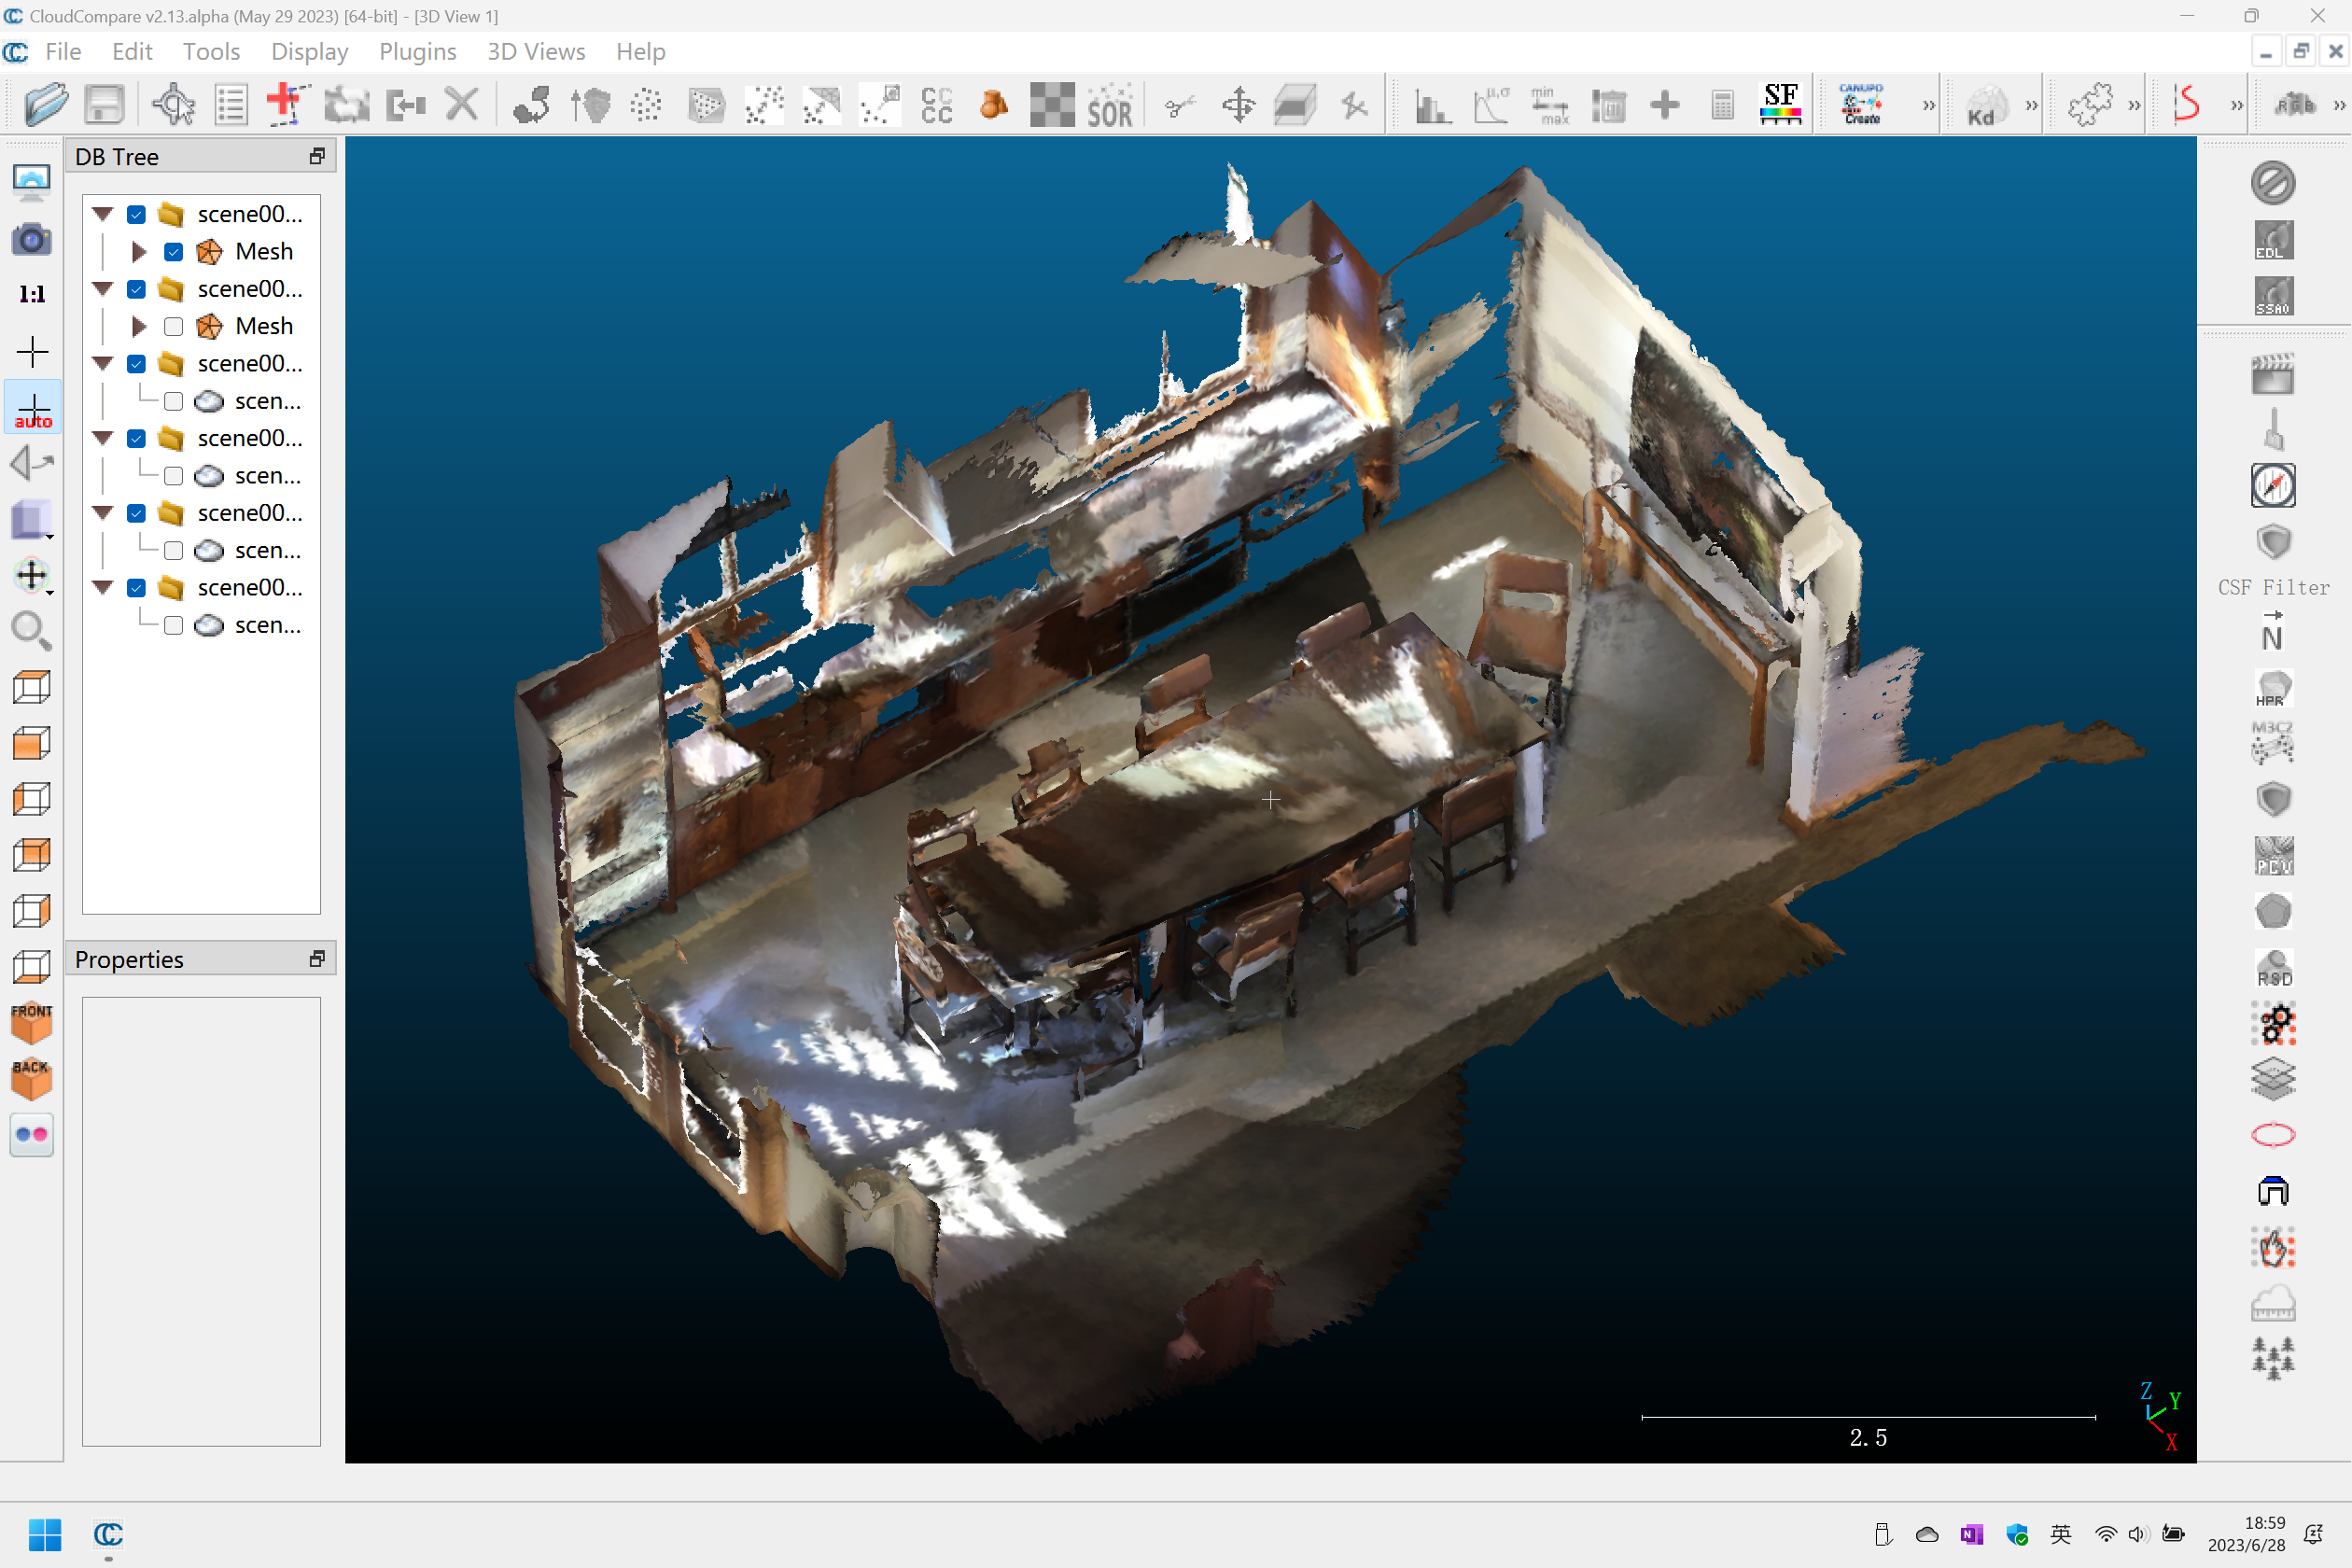
\includegraphics[width=1\textwidth]{figures/result/scene0011_rgb_gt.png}
		\end{minipage}
	}
	\subfigure[语义信息GT模型]{
		\begin{minipage}[t]{0.48\linewidth}
			\centering
			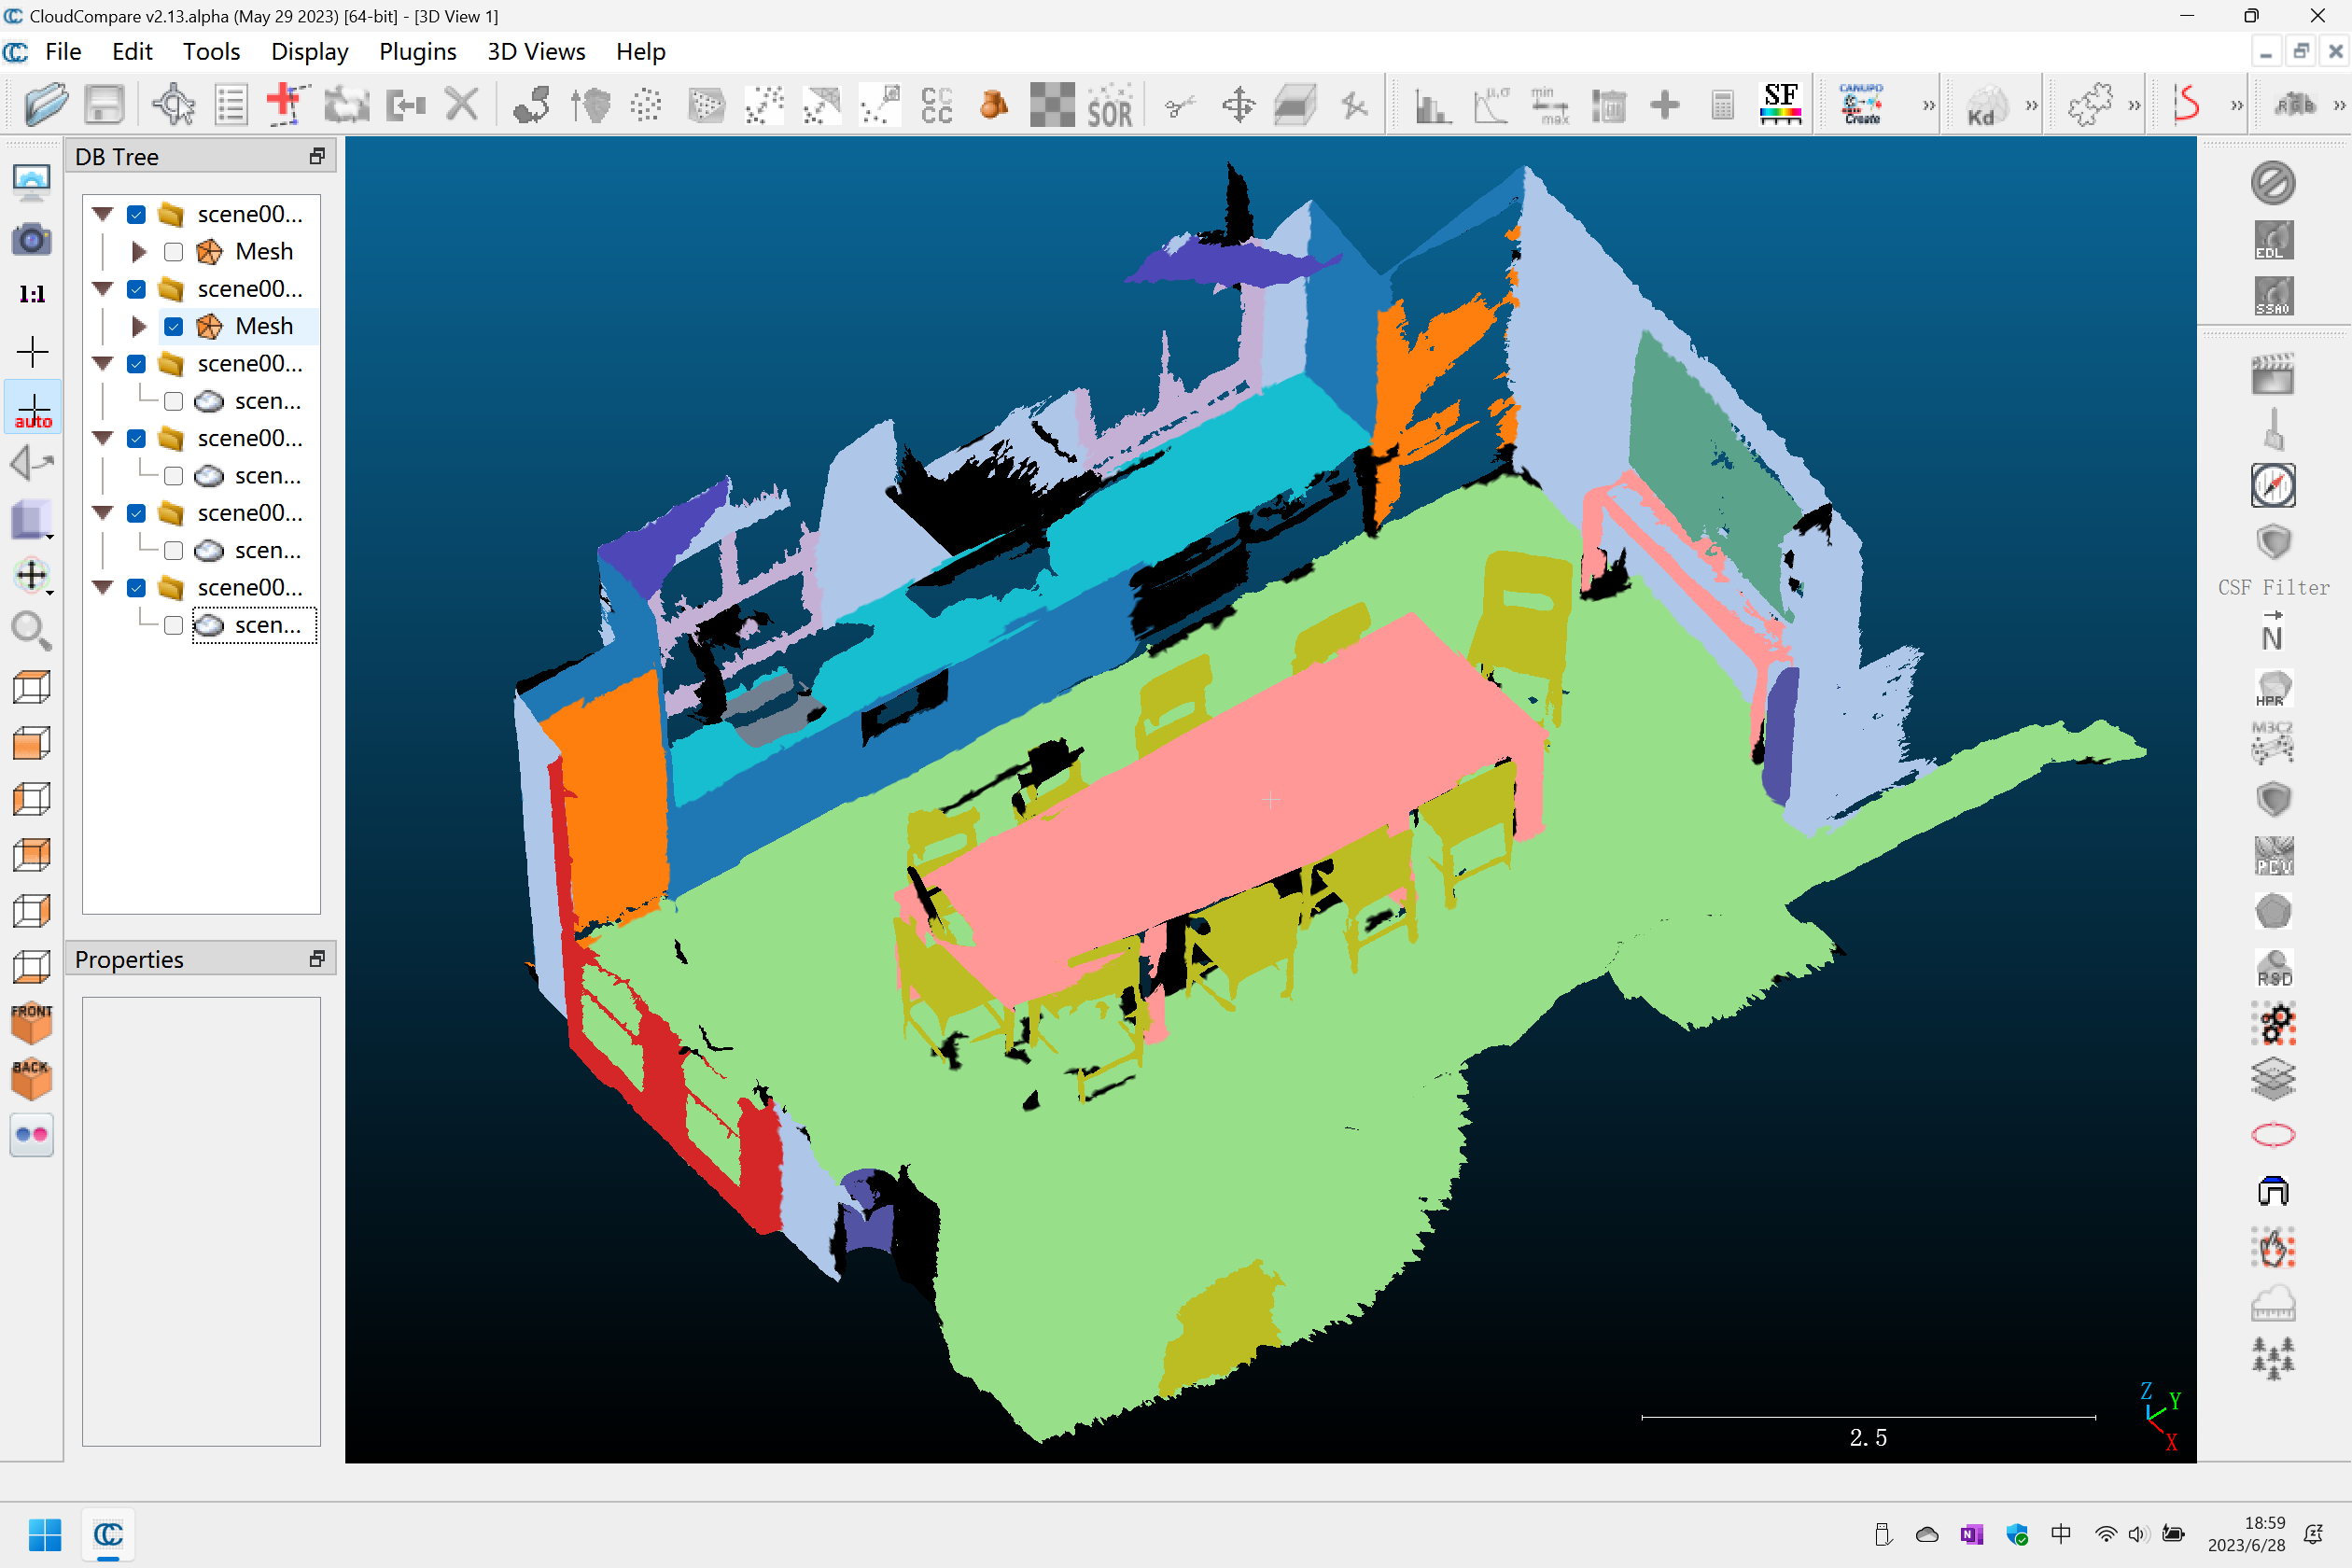
\includegraphics[width=1\textwidth]{figures/result/scene0011_label_gt.png}
		\end{minipage}
	}

	\subfigure[RGB信息2cm模型]{
		\begin{minipage}[t]{0.48\linewidth}
			\centering
			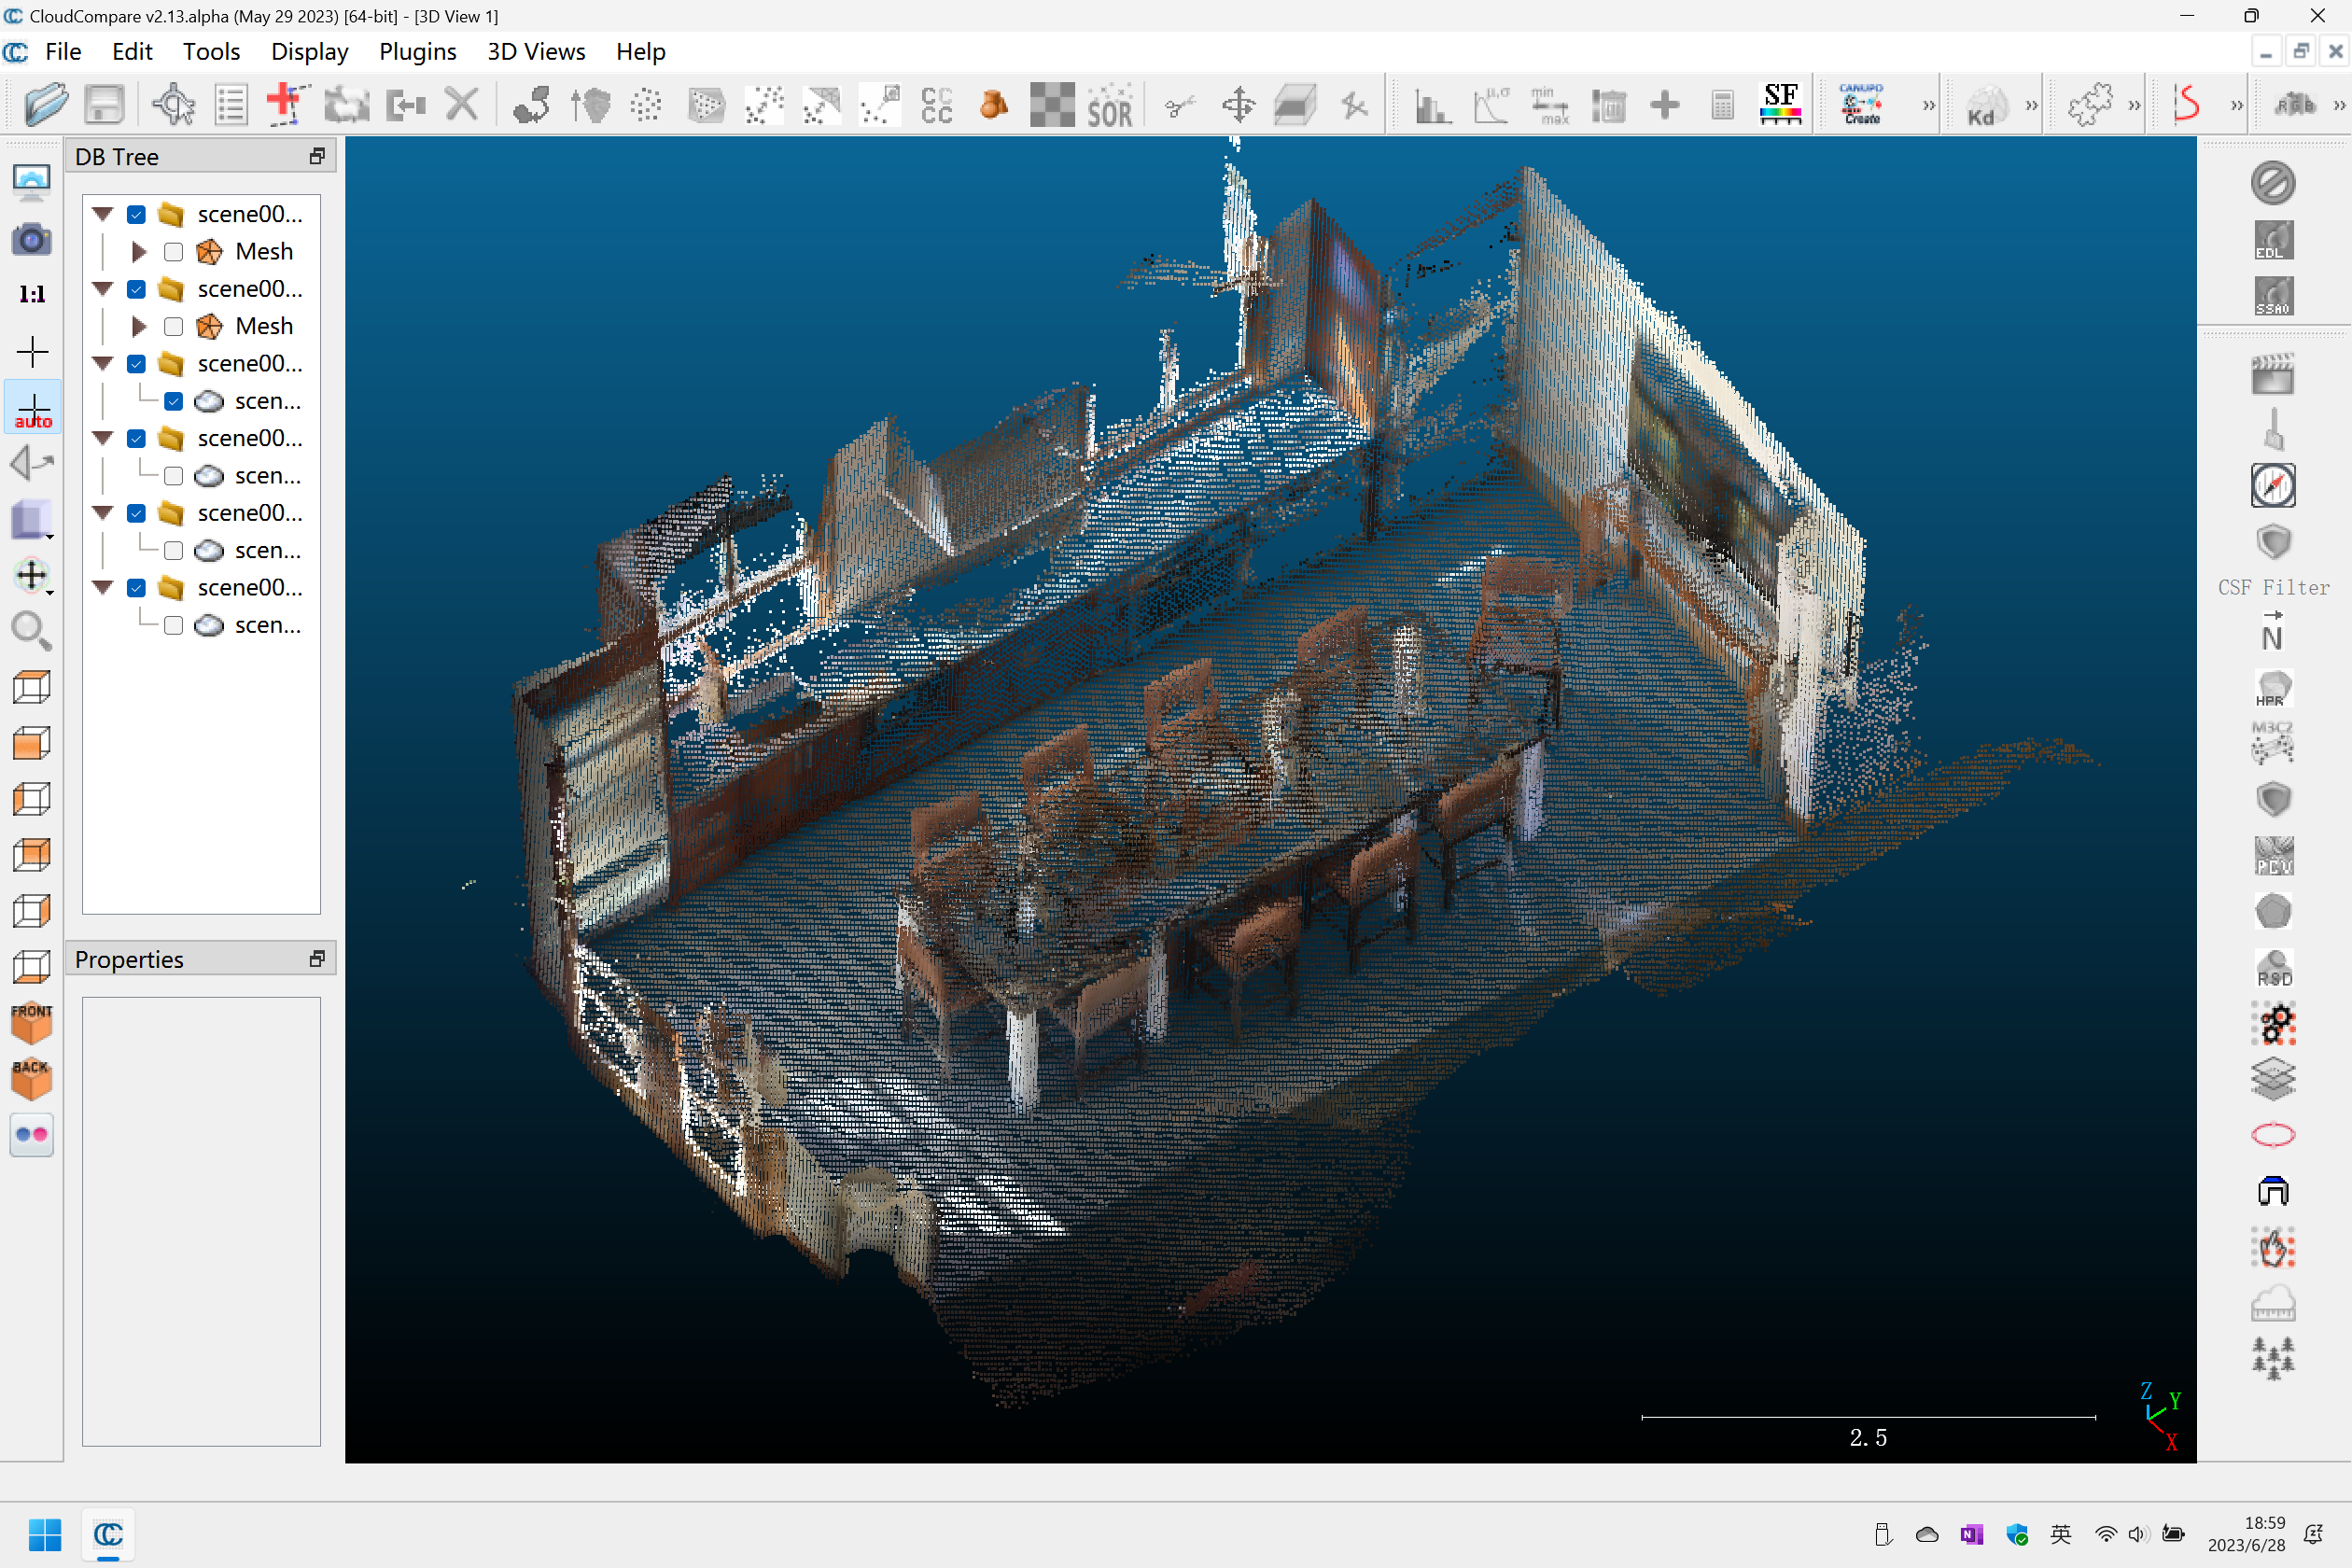
\includegraphics[width=1\textwidth]{figures/result/scene0011_rgb_2cm.png}
		\end{minipage}
	}
	\subfigure[语义信息2cm模型]{
		\begin{minipage}[t]{0.48\linewidth}
			\centering
			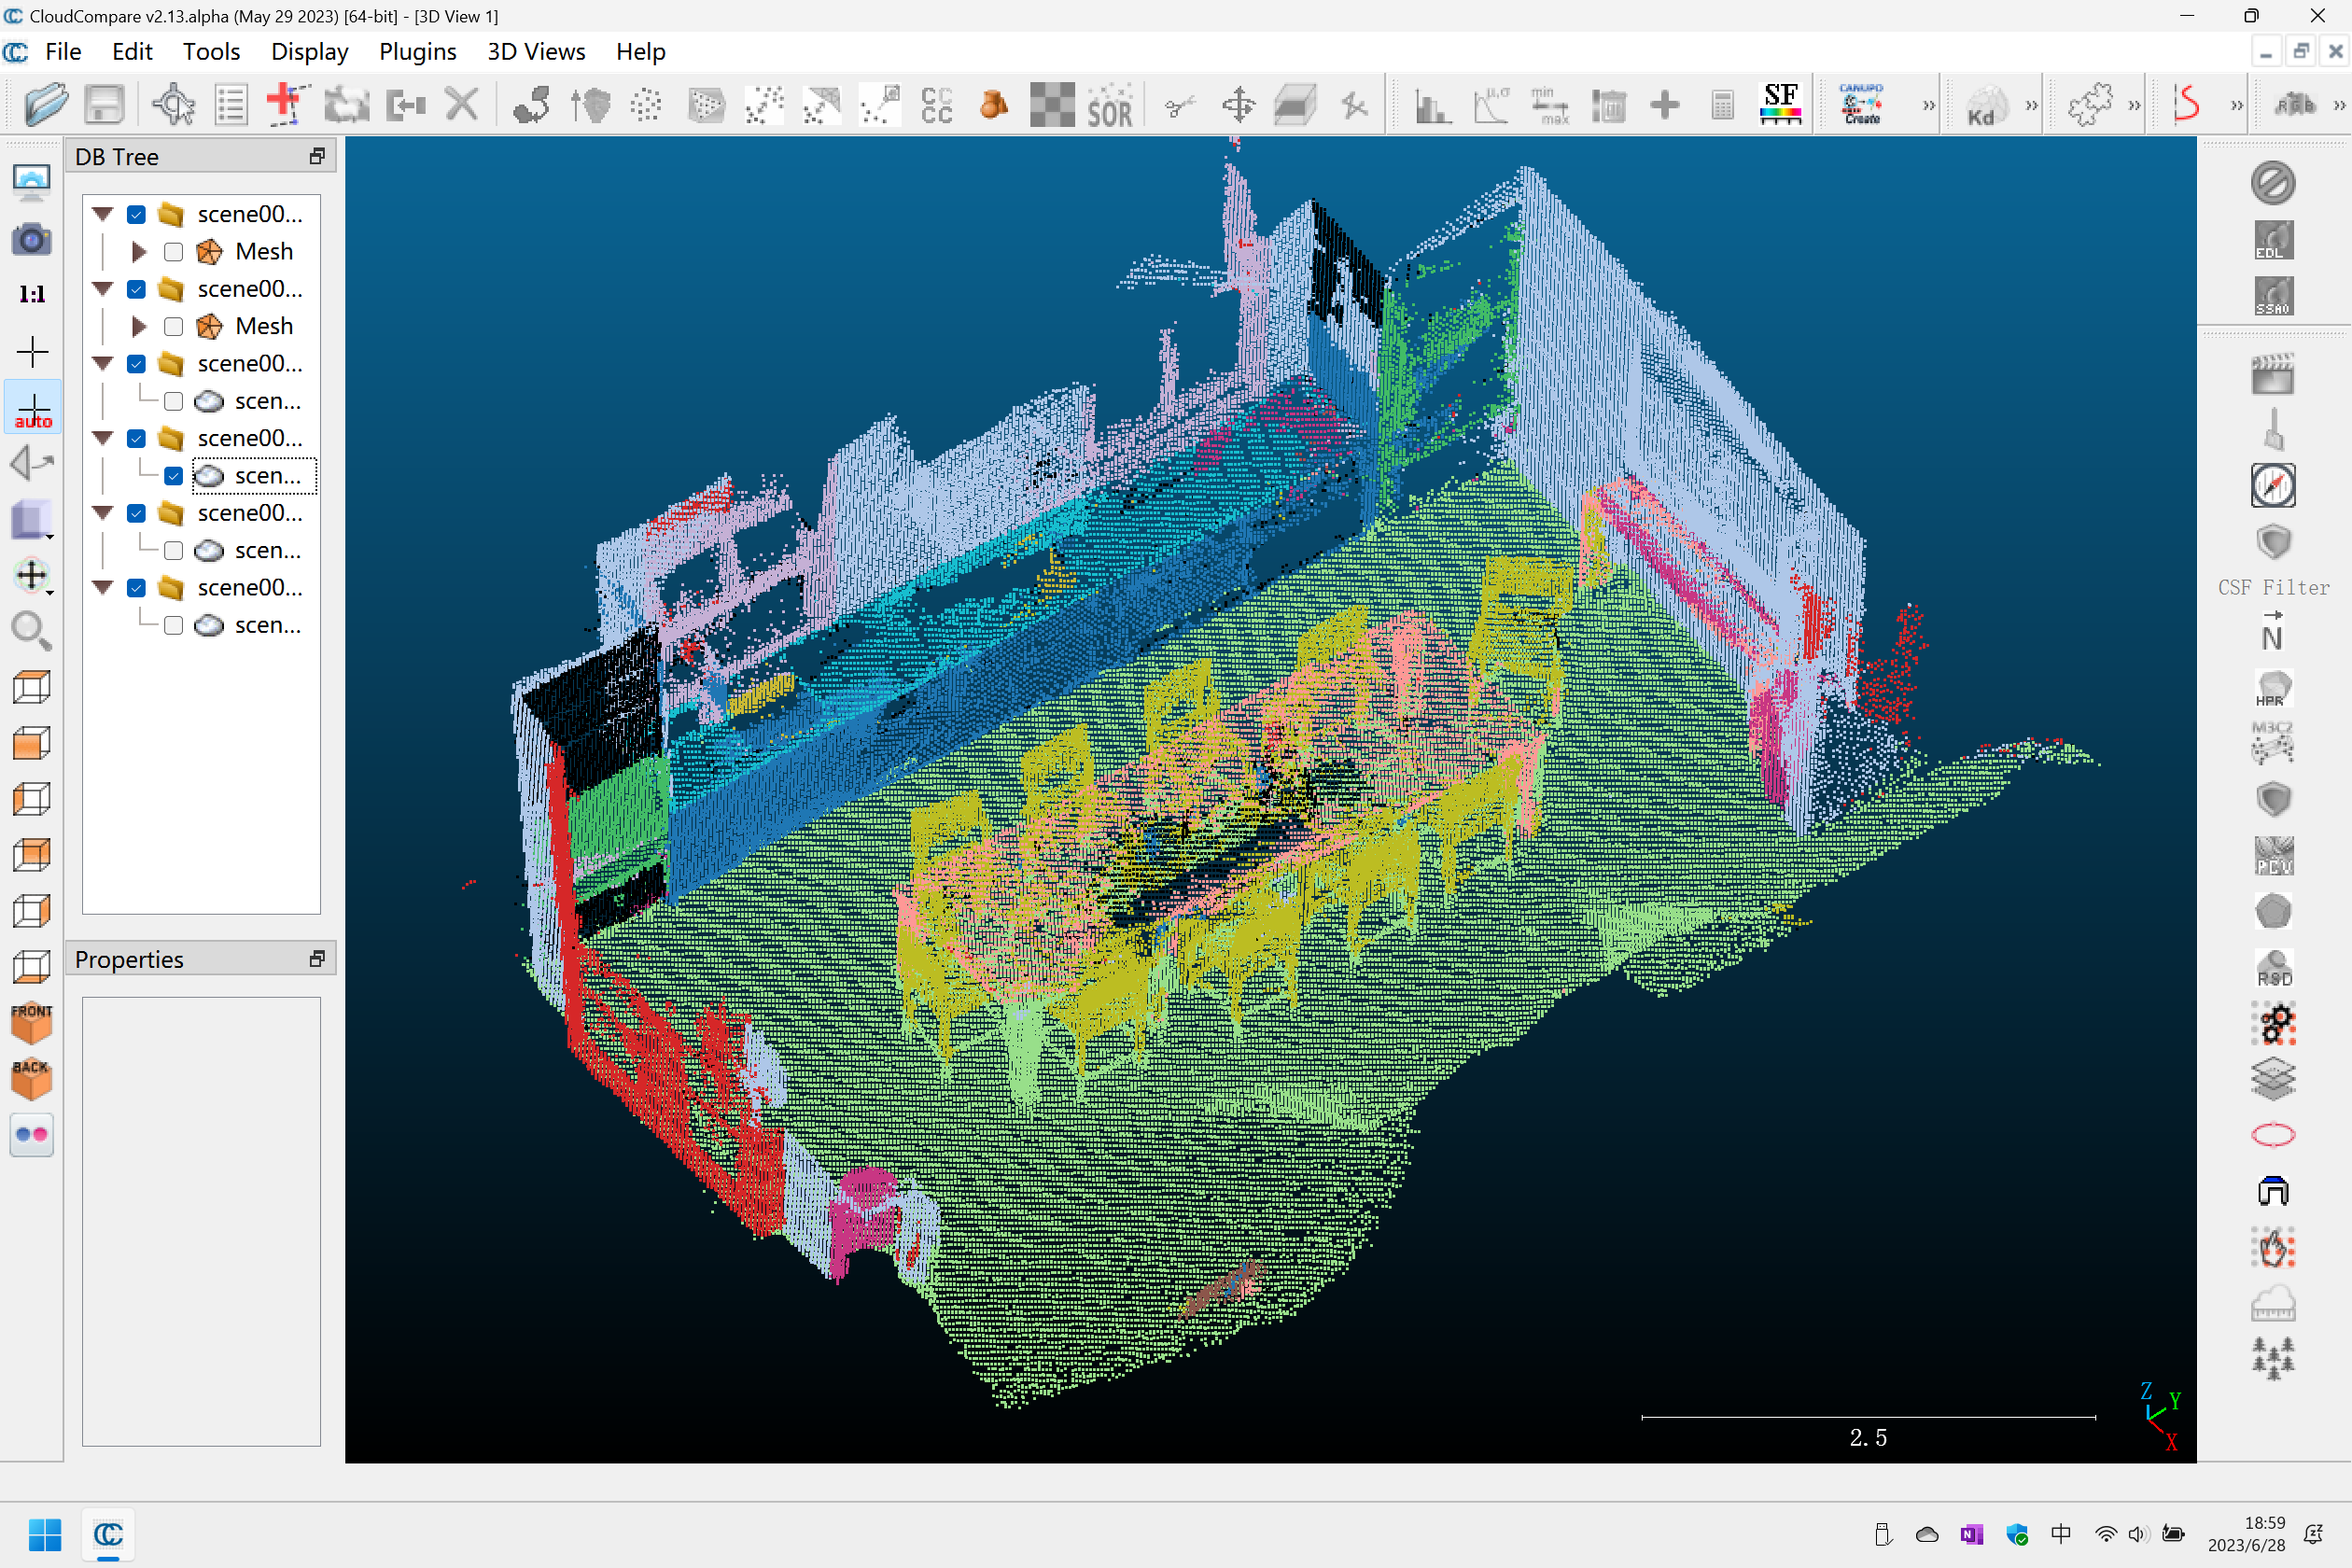
\includegraphics[width=1\textwidth]{figures/result/scene0011_label_2cm.png}
		\end{minipage}
	}

	\subfigure[RGB信息5cm模型]{
		\begin{minipage}[t]{0.48\linewidth}
			\centering
			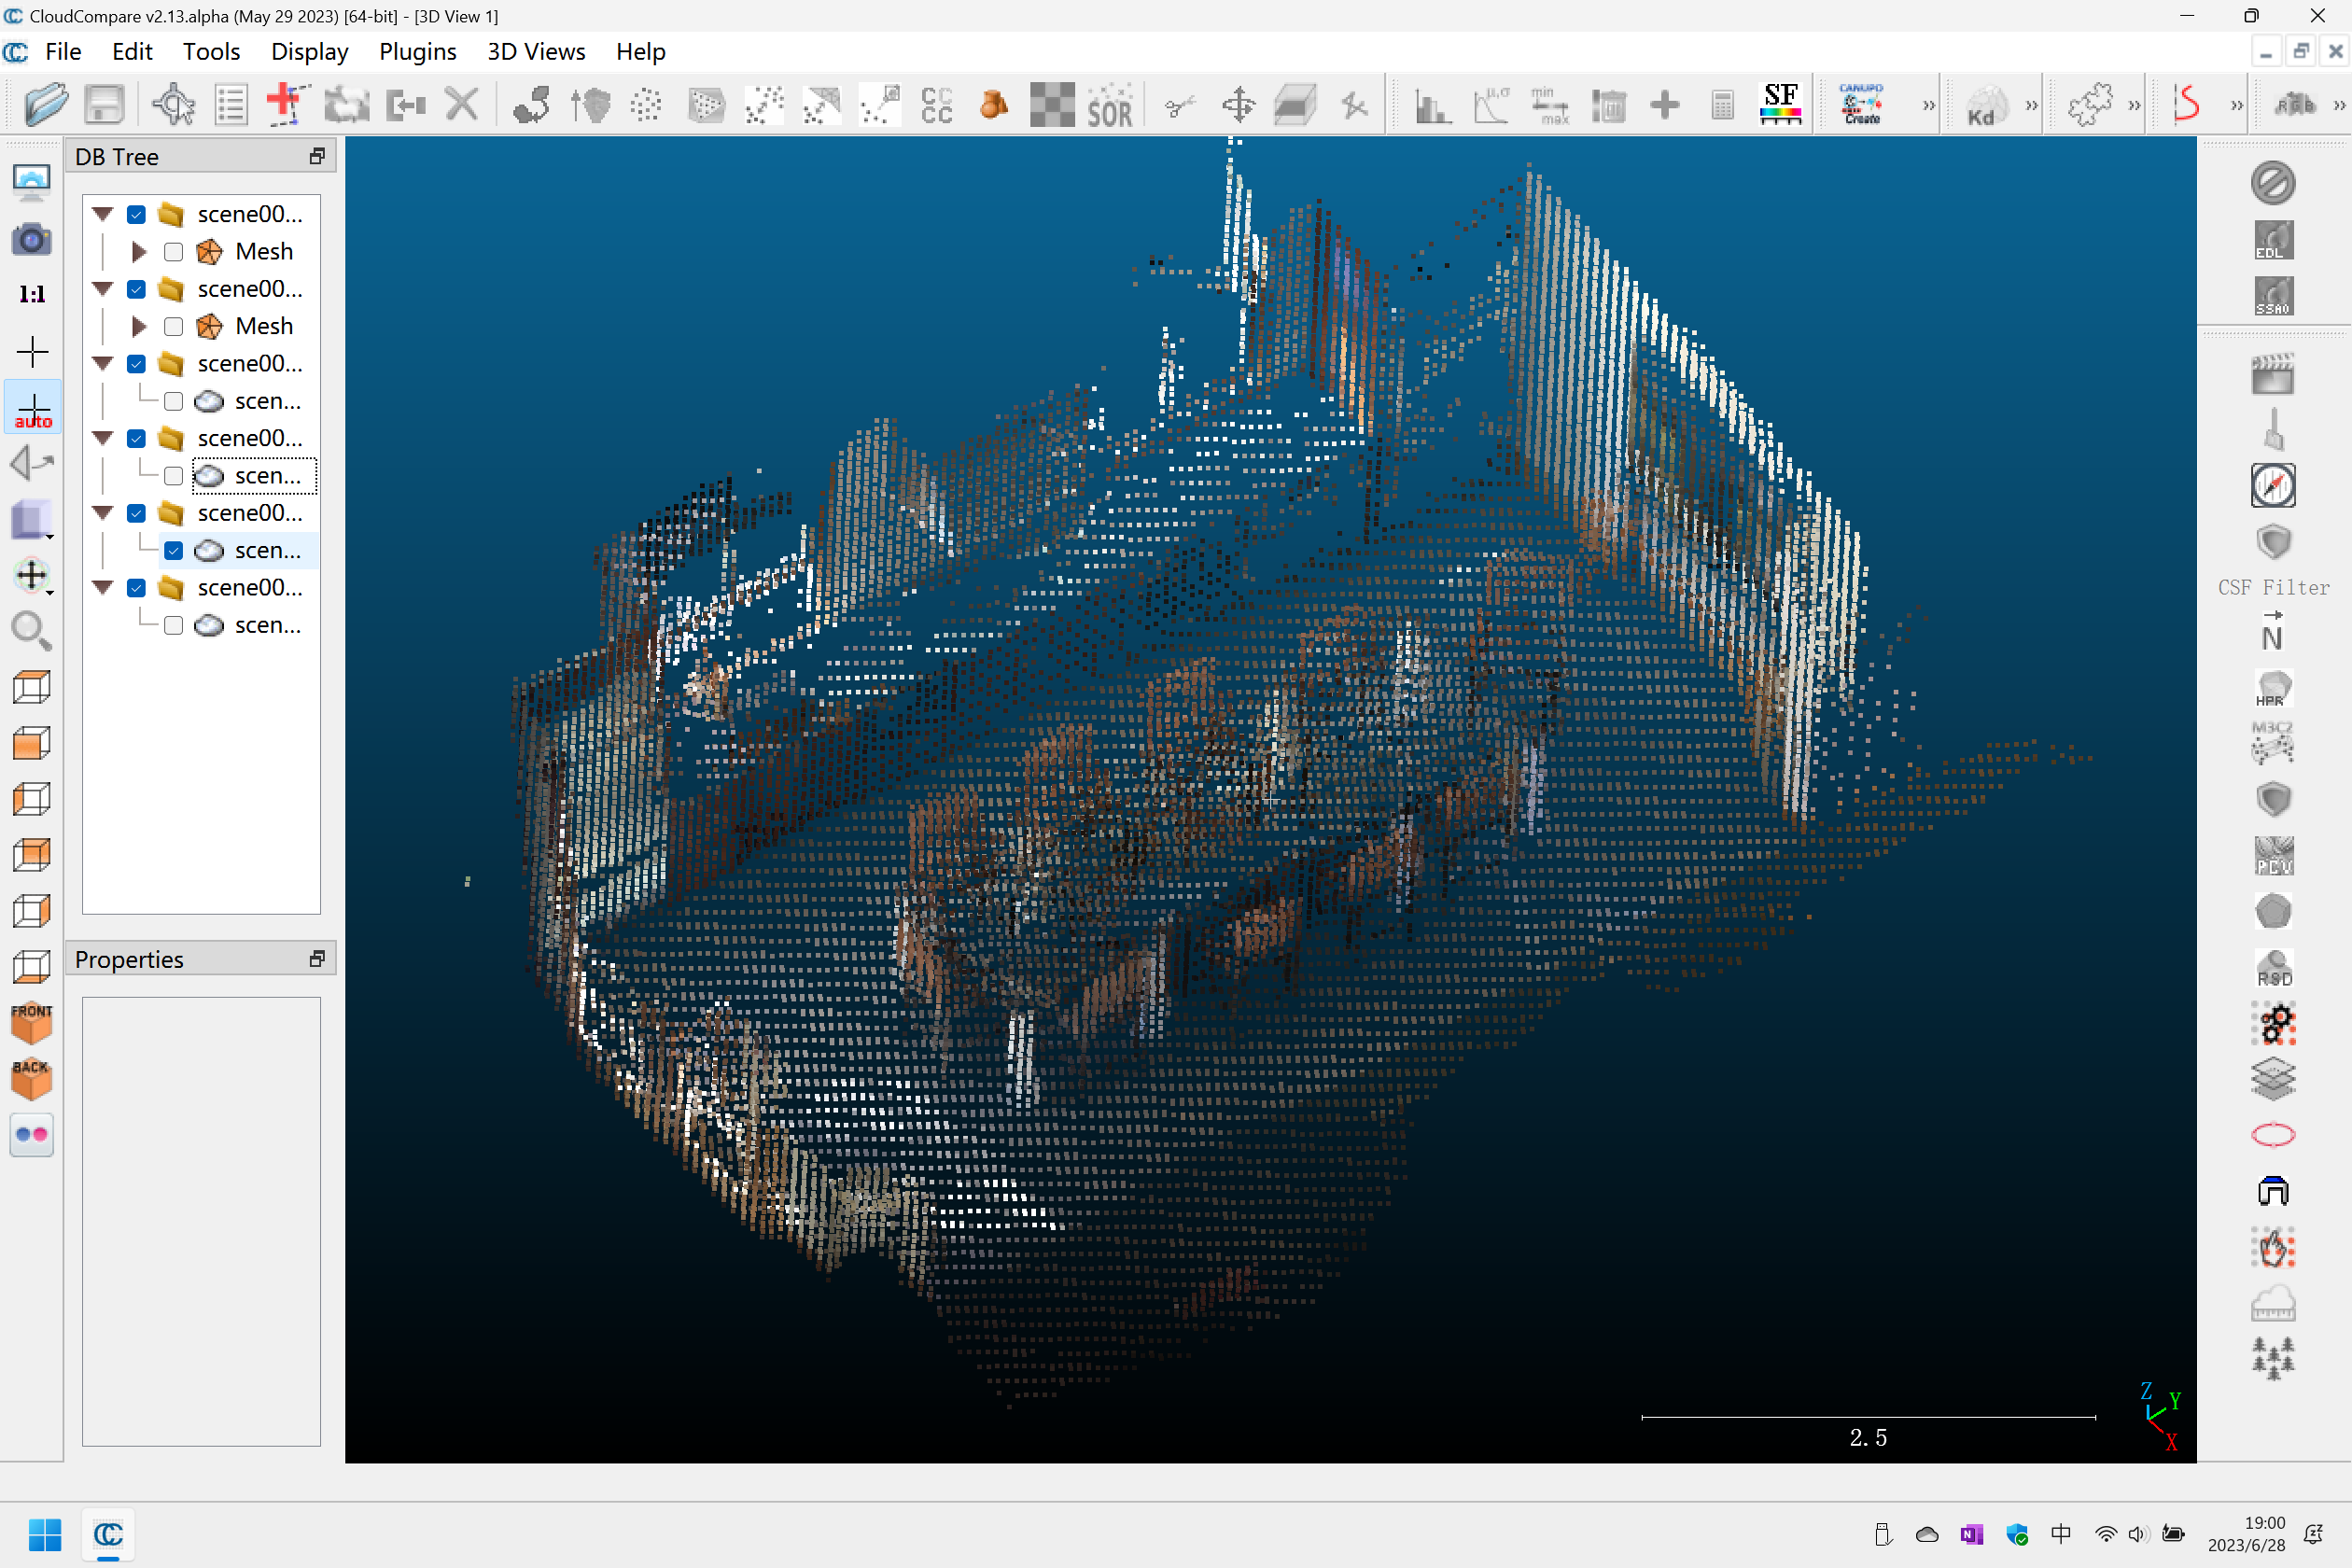
\includegraphics[width=1\textwidth]{figures/result/scene0011_rgb_5cm.png}
		\end{minipage}
	}
	\subfigure[语义信息5cm模型]{
		\begin{minipage}[t]{0.48\linewidth}
			\centering
			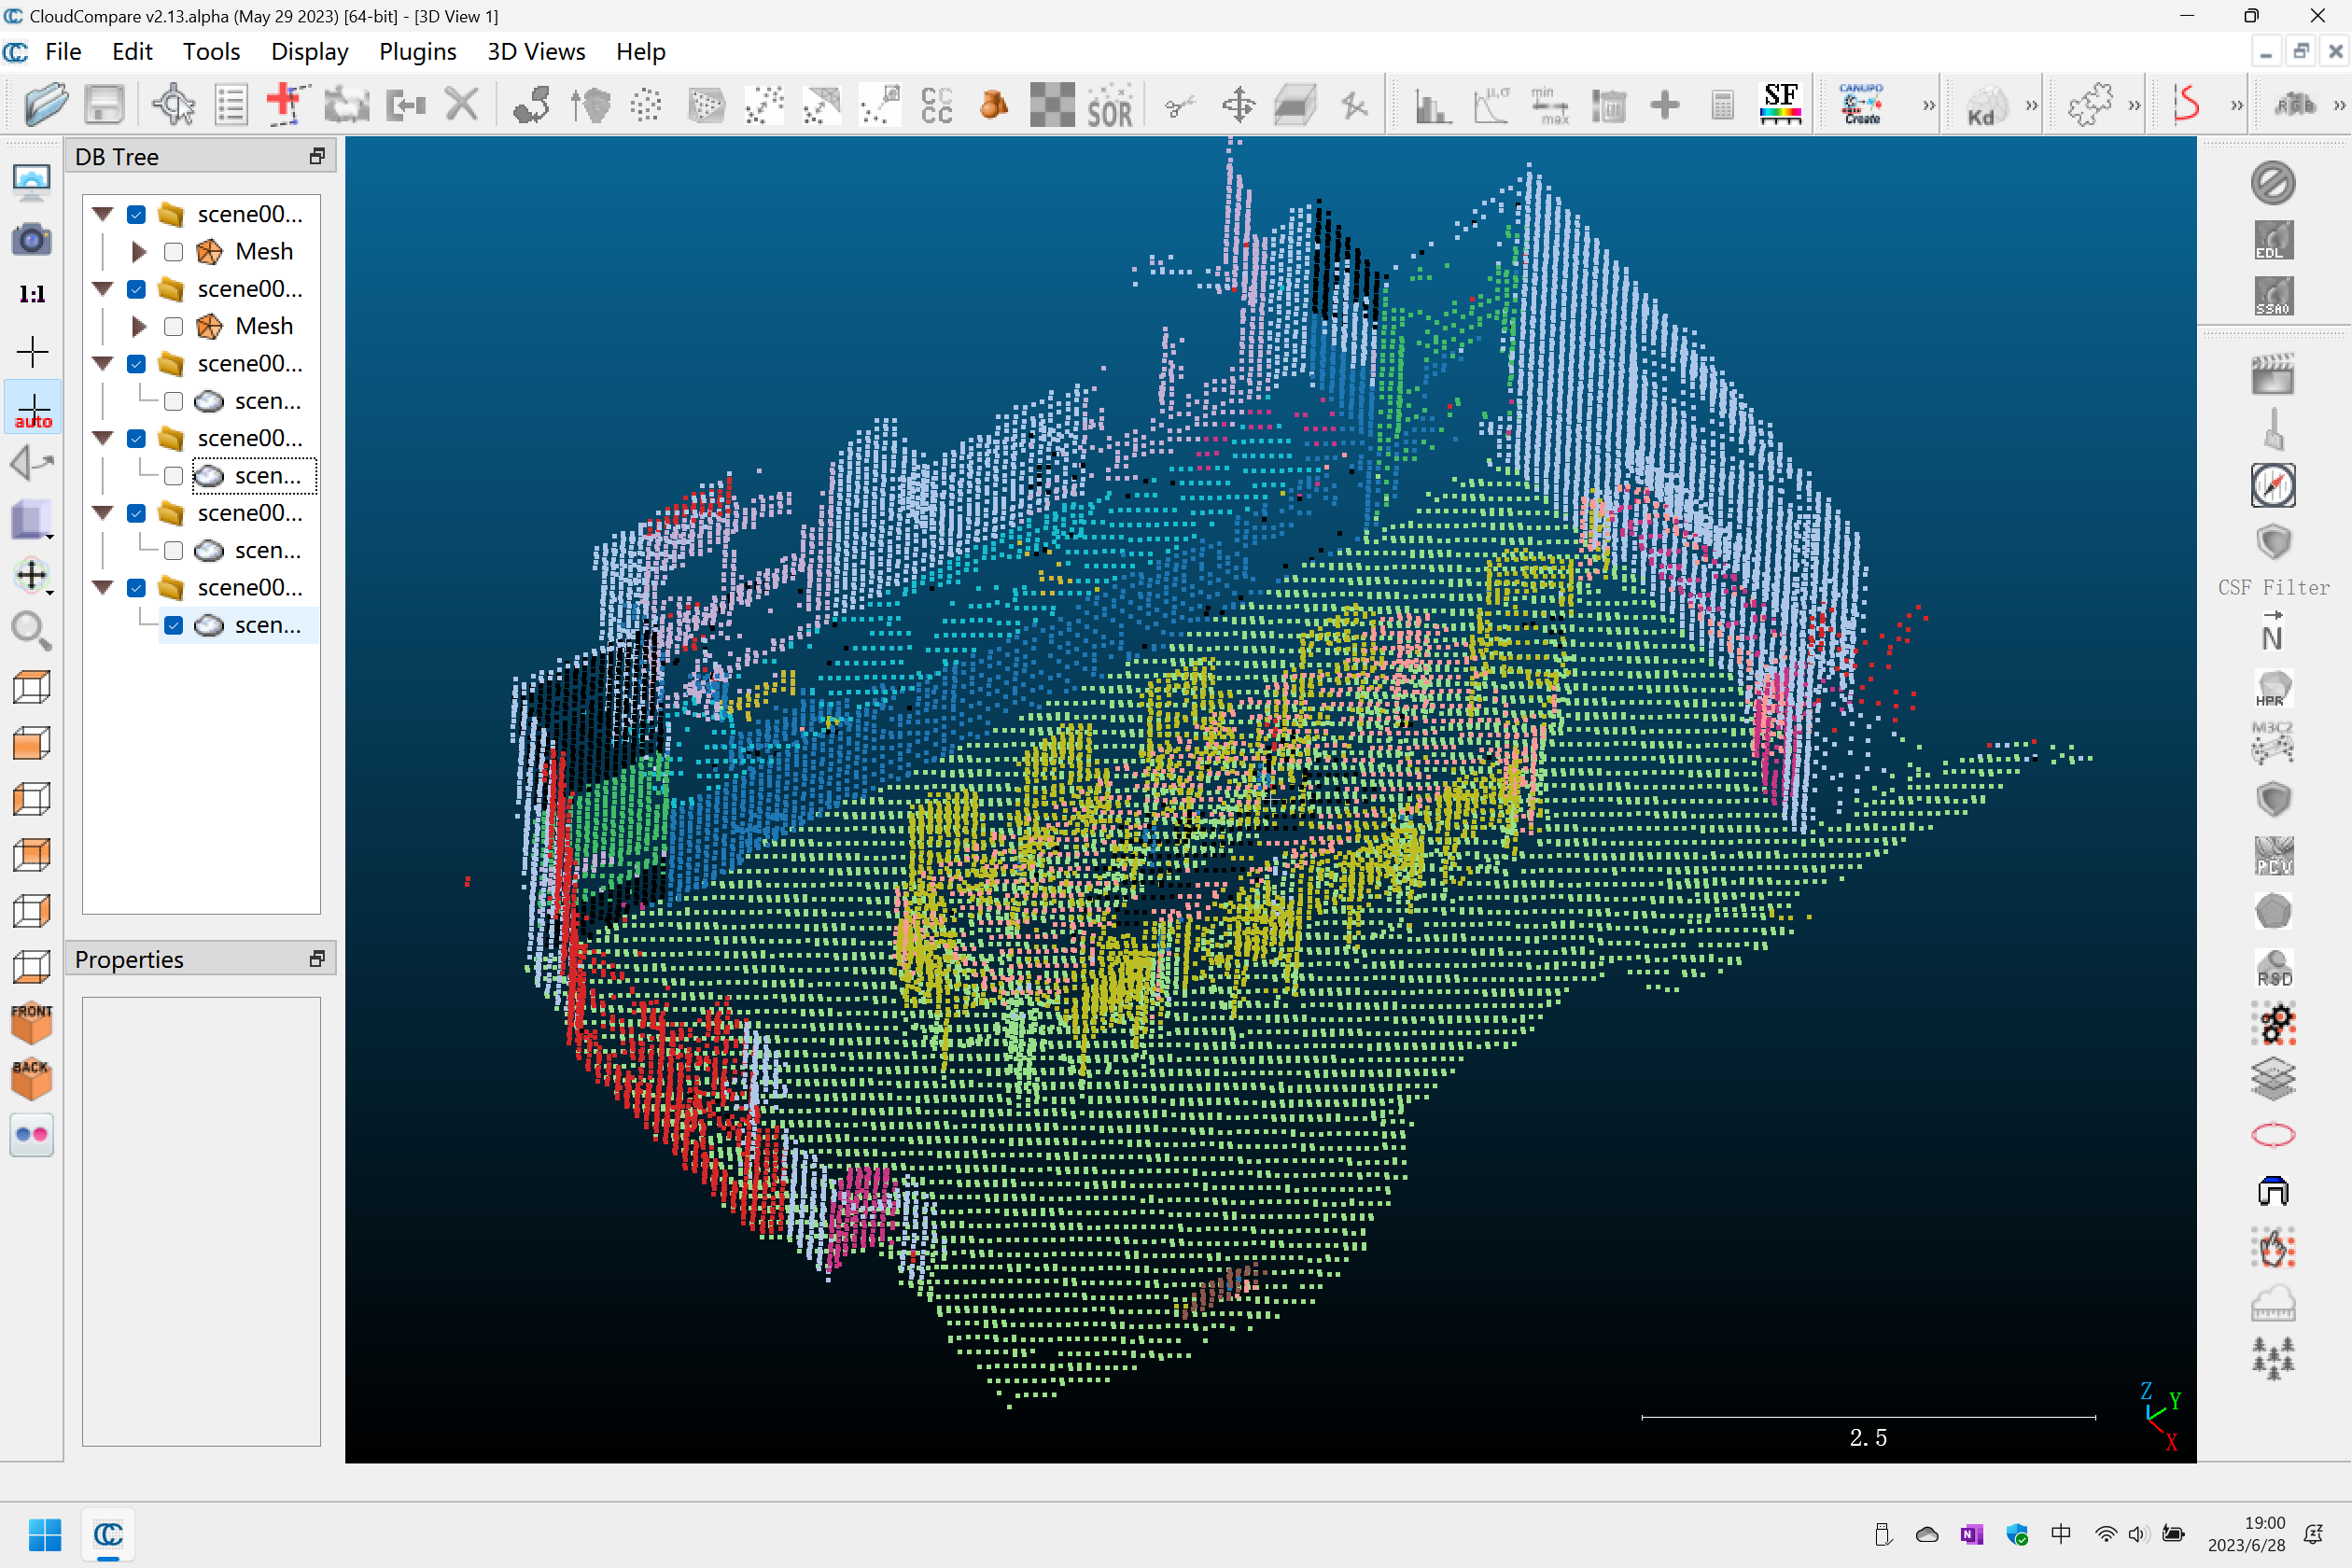
\includegraphics[width=1\textwidth]{figures/result/scene0011_label_5cm.png}
		\end{minipage}
	}
	\caption{场景scene0011\_00导出结果}
	\label{fig:scene0011_00_result}
\end{figure}

\begin{figure}
	\centering
	\subfigure[RGB信息GT模型]{
		\begin{minipage}[t]{0.48\linewidth}
			\centering
			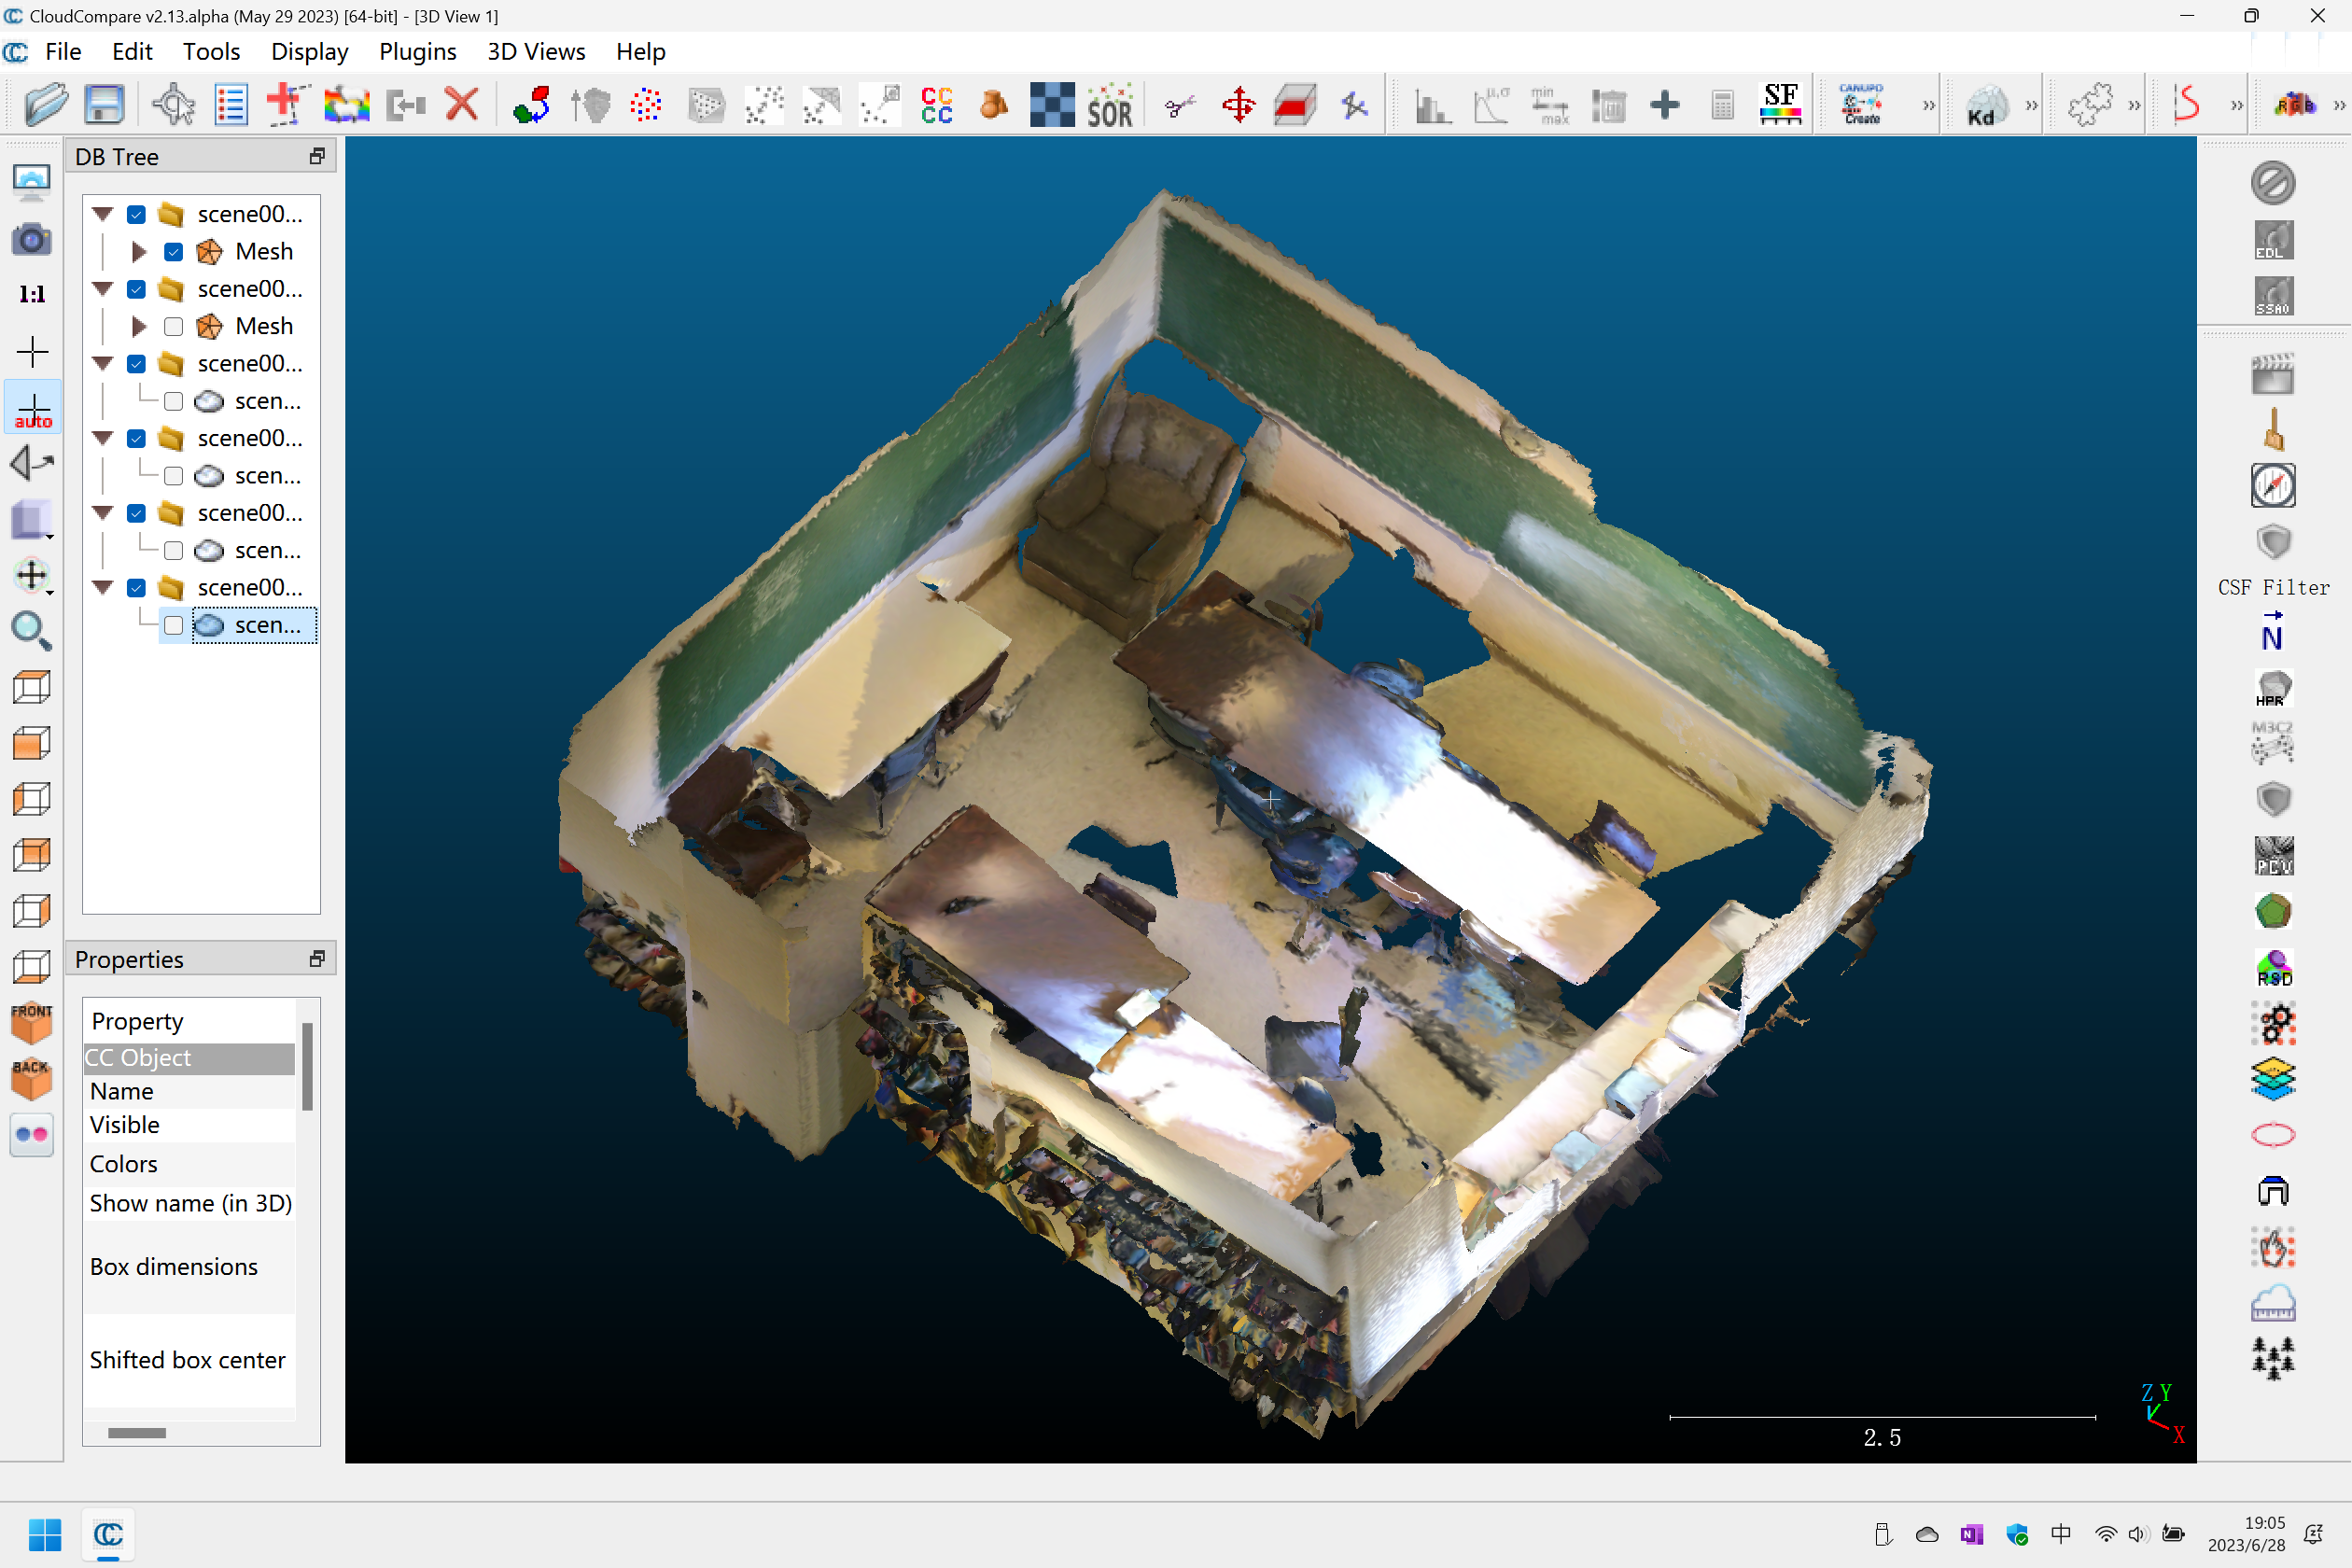
\includegraphics[width=1\textwidth]{figures/result/scene0030_rgb_gt.png}
		\end{minipage}
	}
	\subfigure[语义信息GT模型]{
		\begin{minipage}[t]{0.48\linewidth}
			\centering
			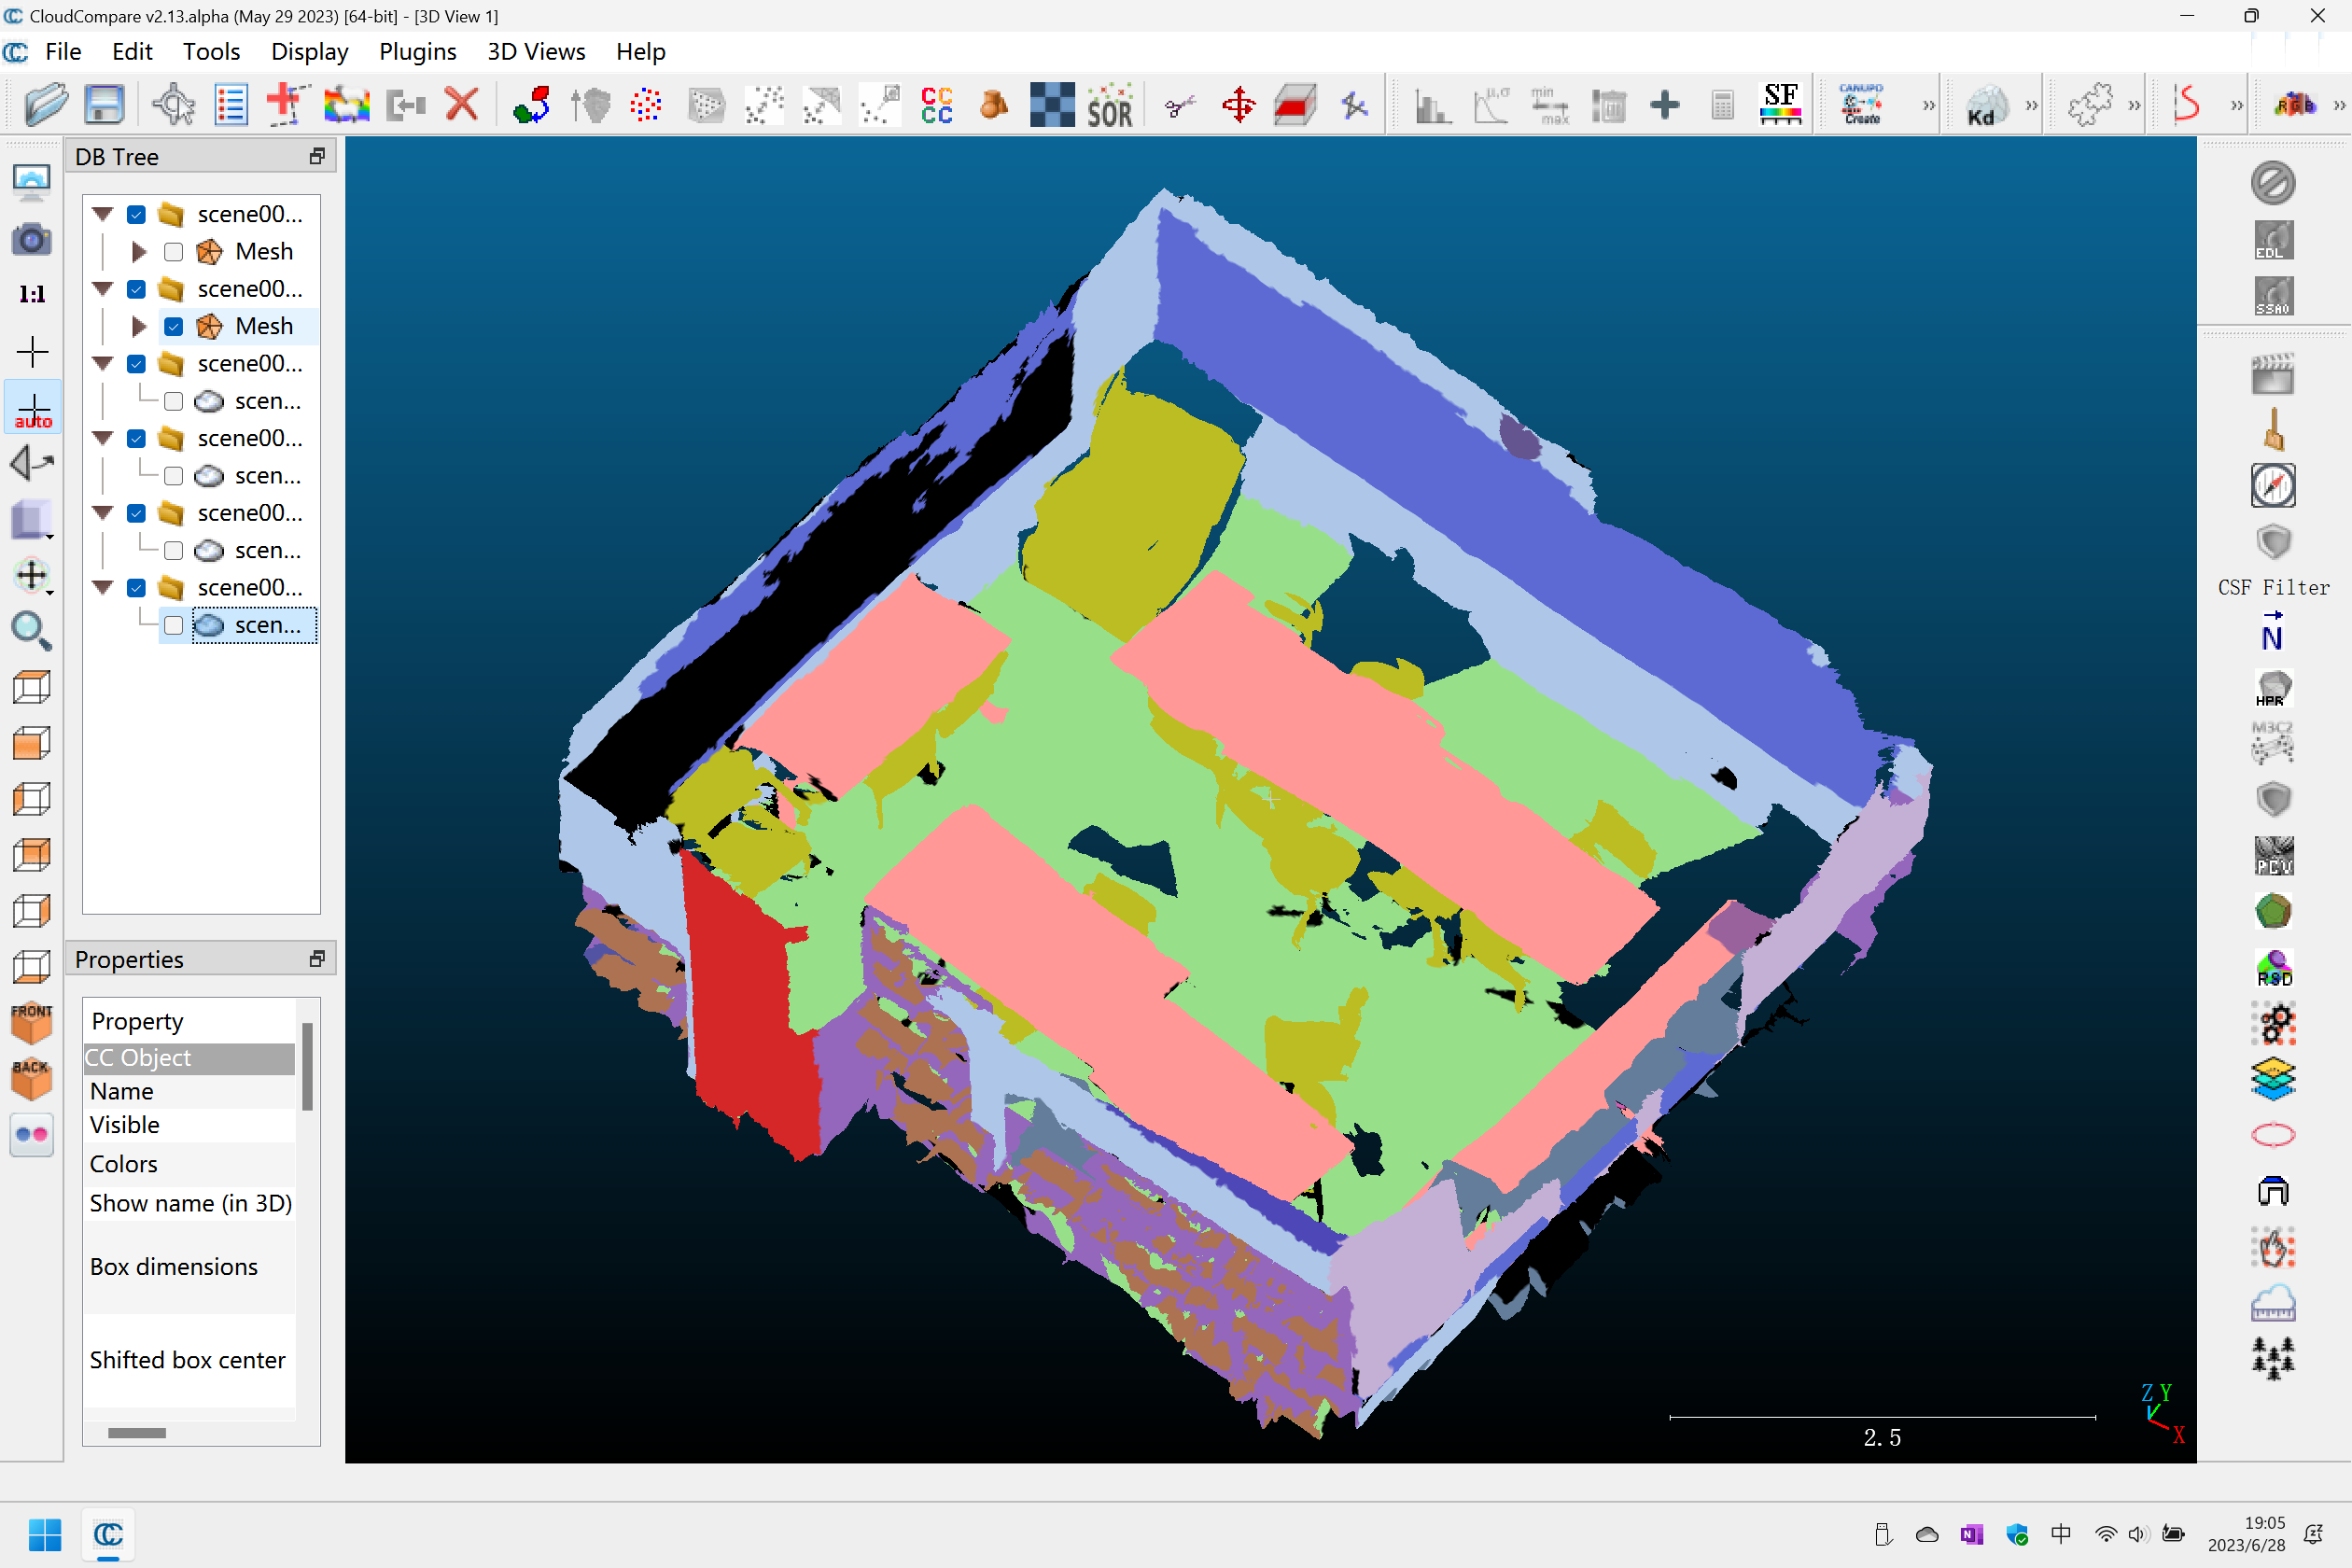
\includegraphics[width=1\textwidth]{figures/result/scene0030_label_gt.png}
		\end{minipage}
	}

	\subfigure[RGB信息2cm模型]{
		\begin{minipage}[t]{0.48\linewidth}
			\centering
			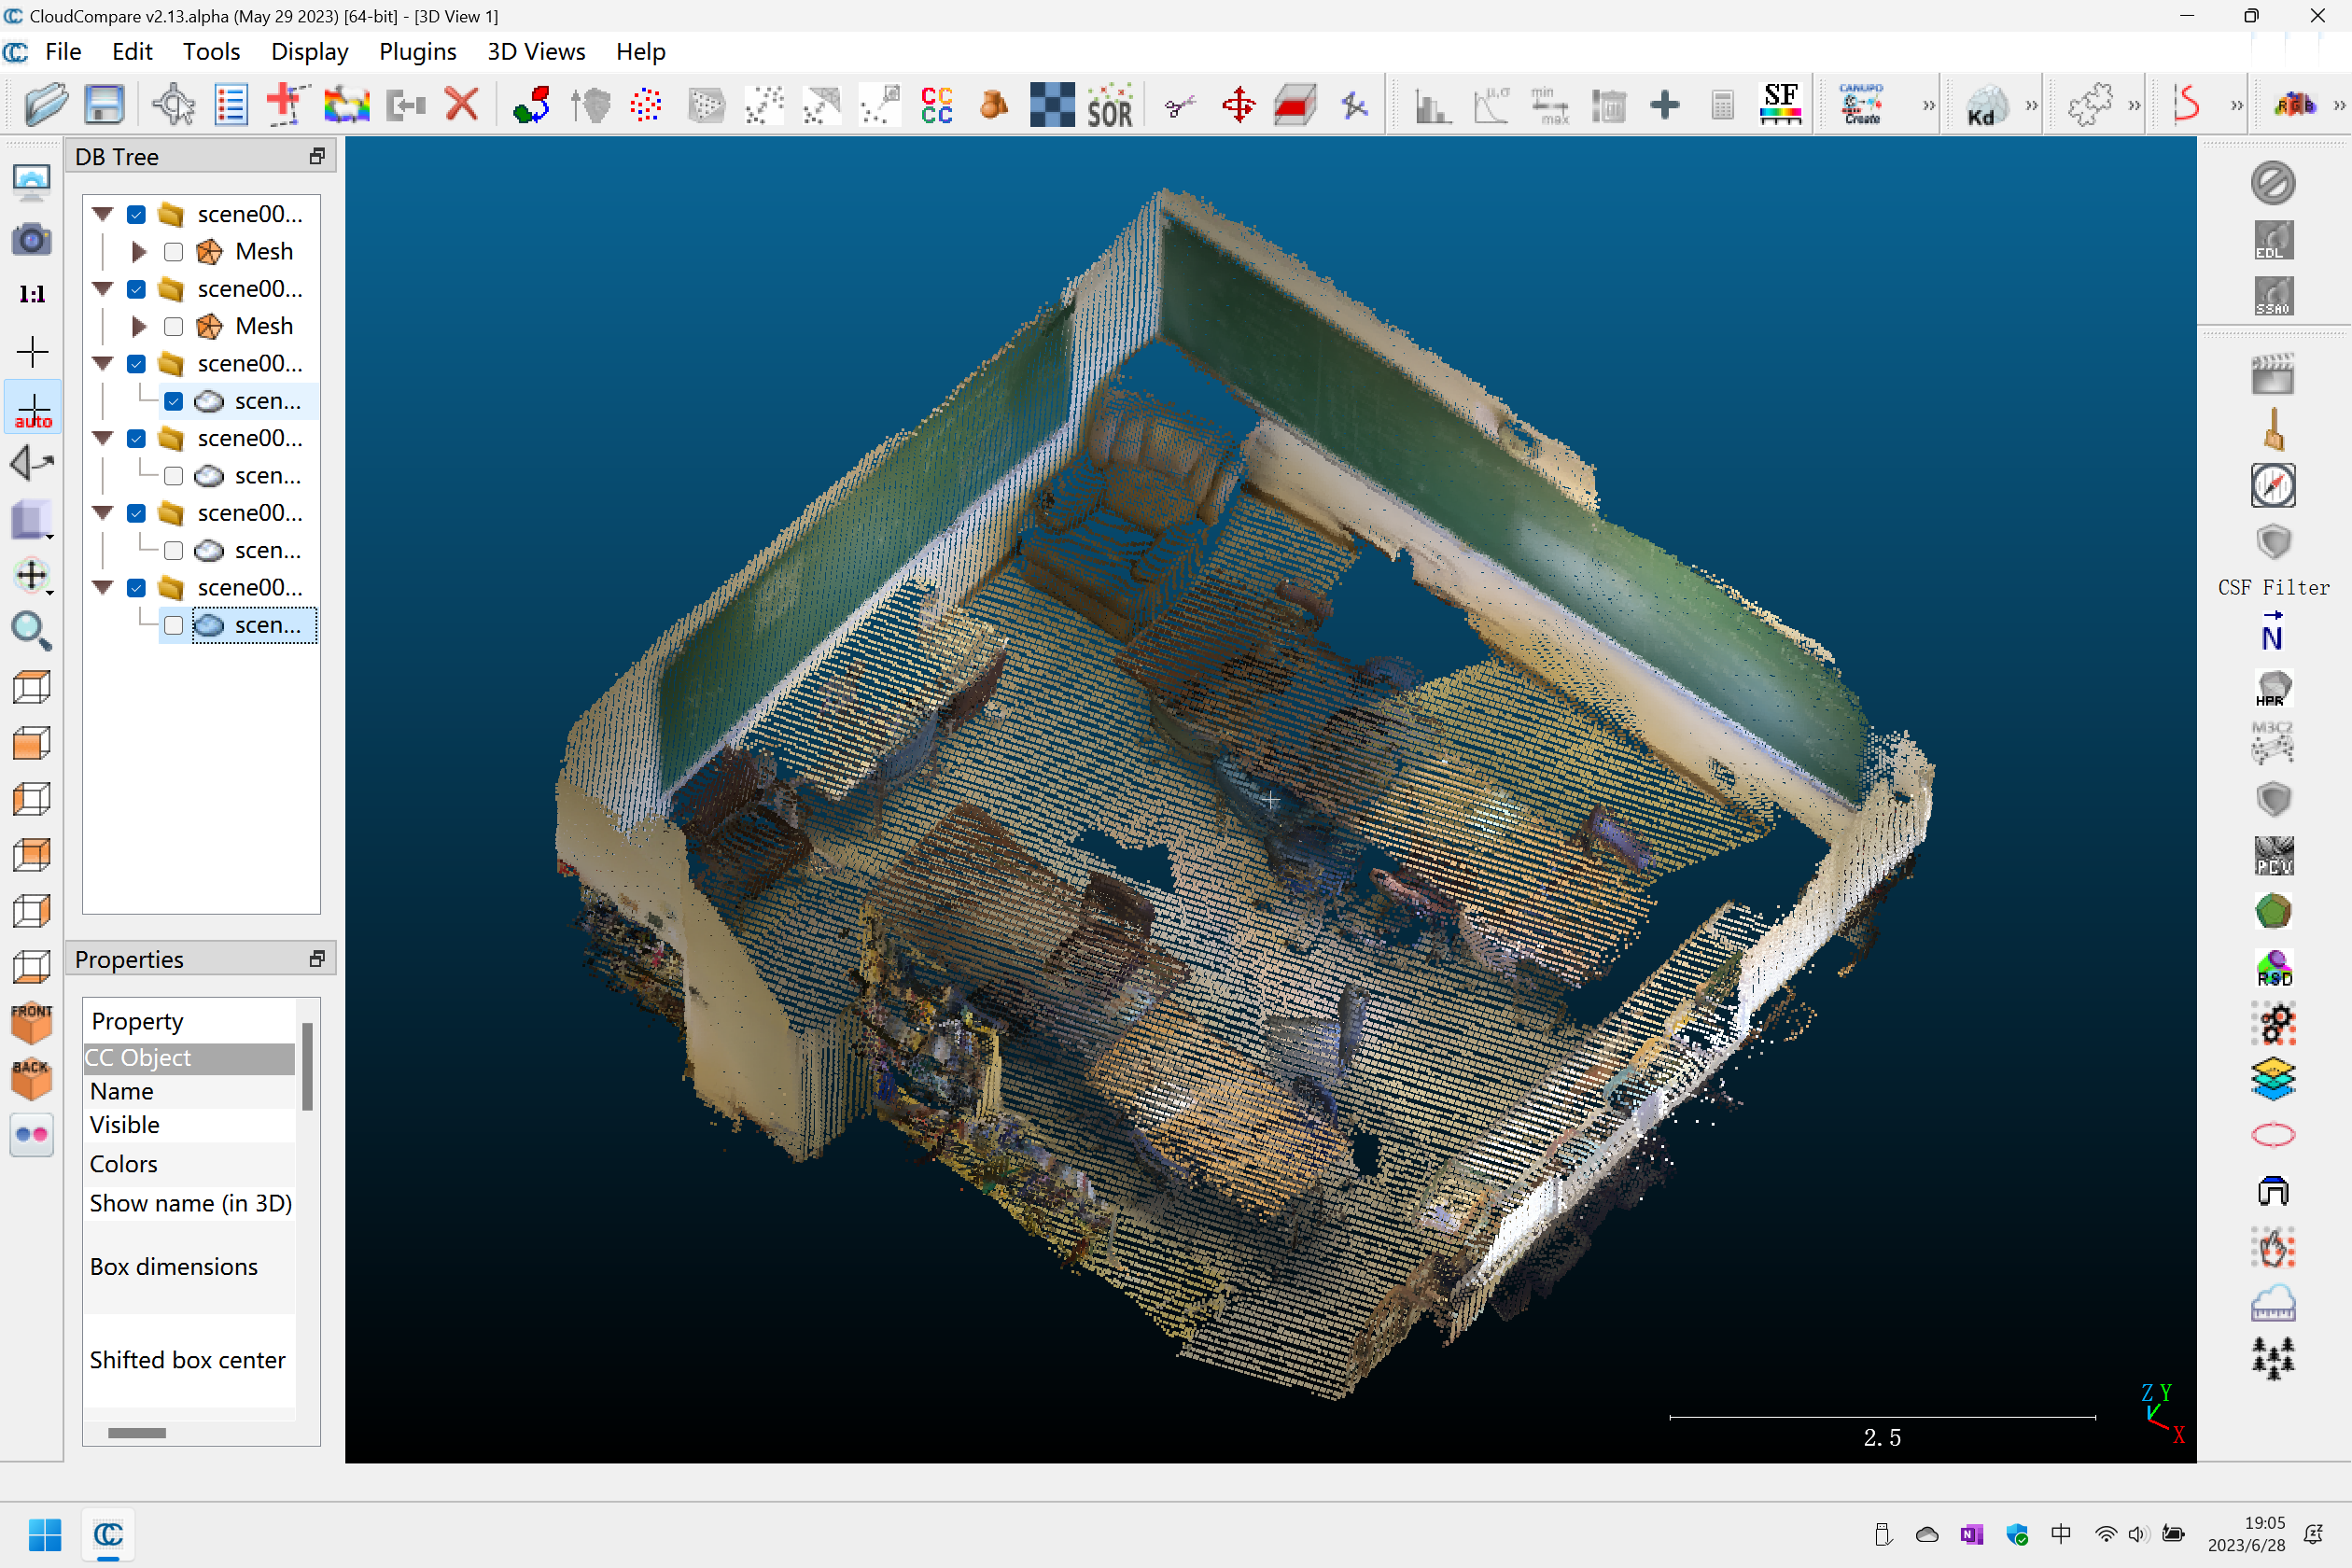
\includegraphics[width=1\textwidth]{figures/result/scene0030_rgb_2cm.png}
		\end{minipage}
	}
	\subfigure[语义信息2cm模型]{
		\begin{minipage}[t]{0.48\linewidth}
			\centering
			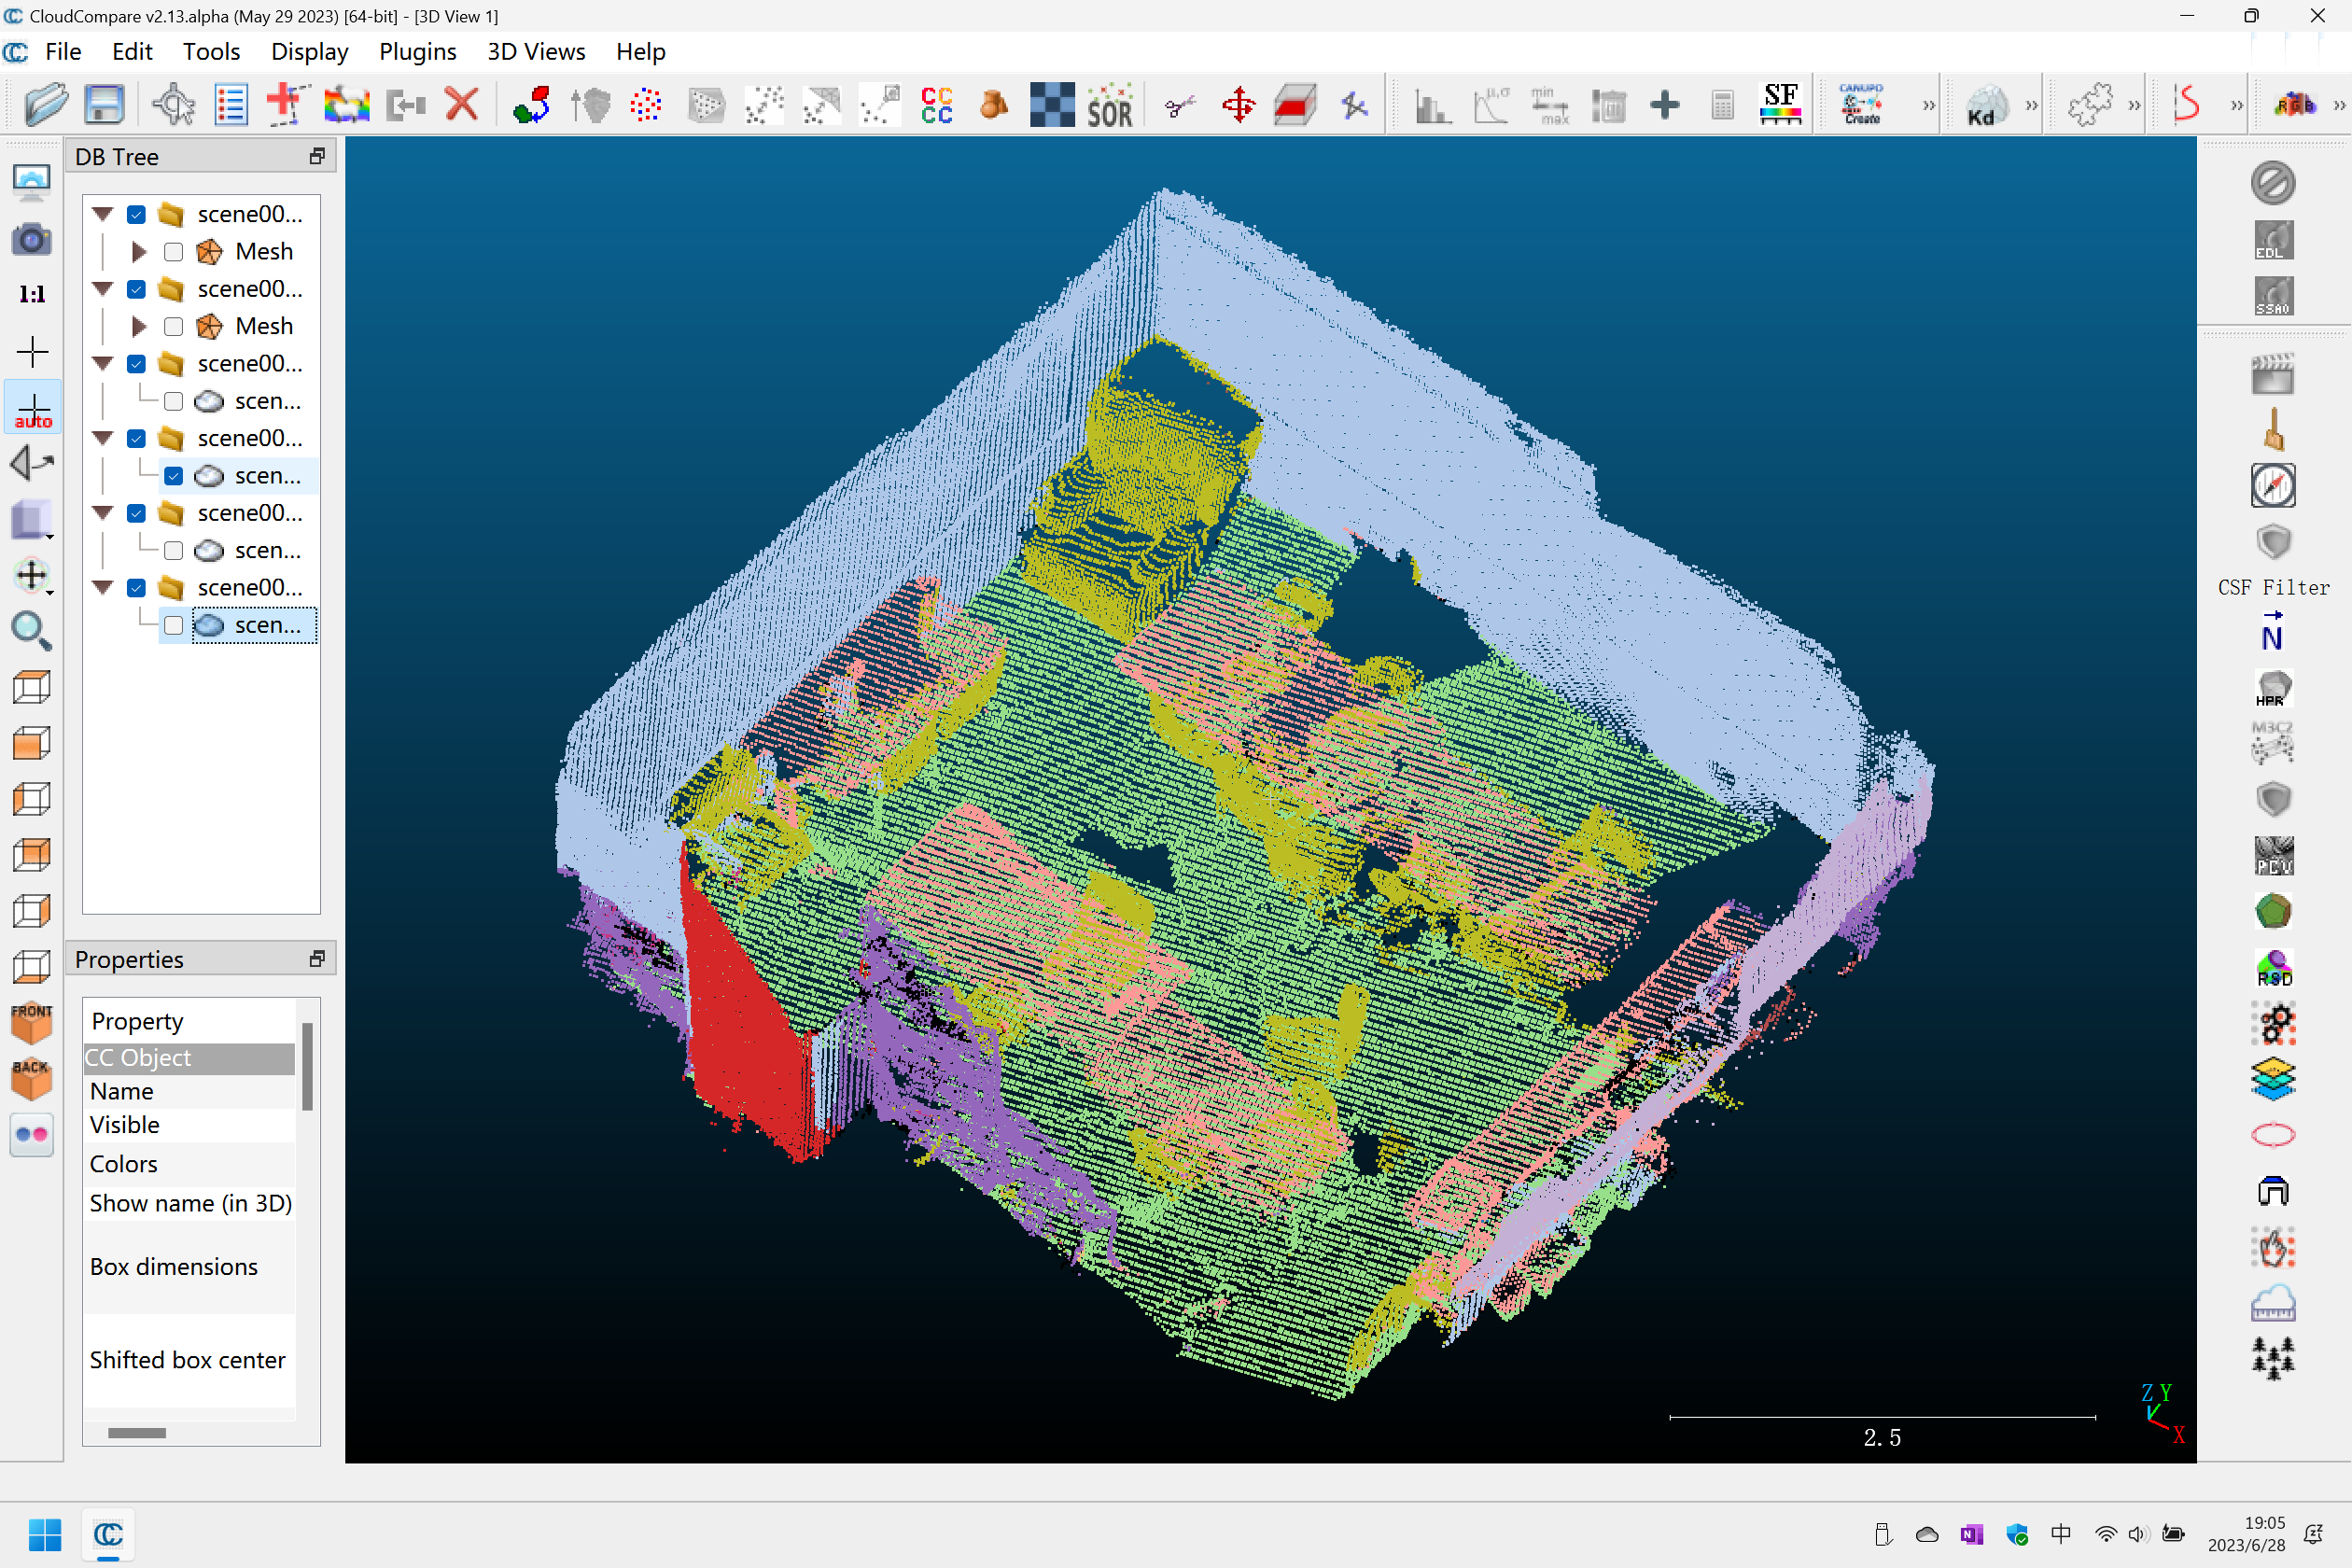
\includegraphics[width=1\textwidth]{figures/result/scene0030_label_2cm.png}
		\end{minipage}
	}

	\subfigure[RGB信息5cm模型]{
		\begin{minipage}[t]{0.48\linewidth}
			\centering
			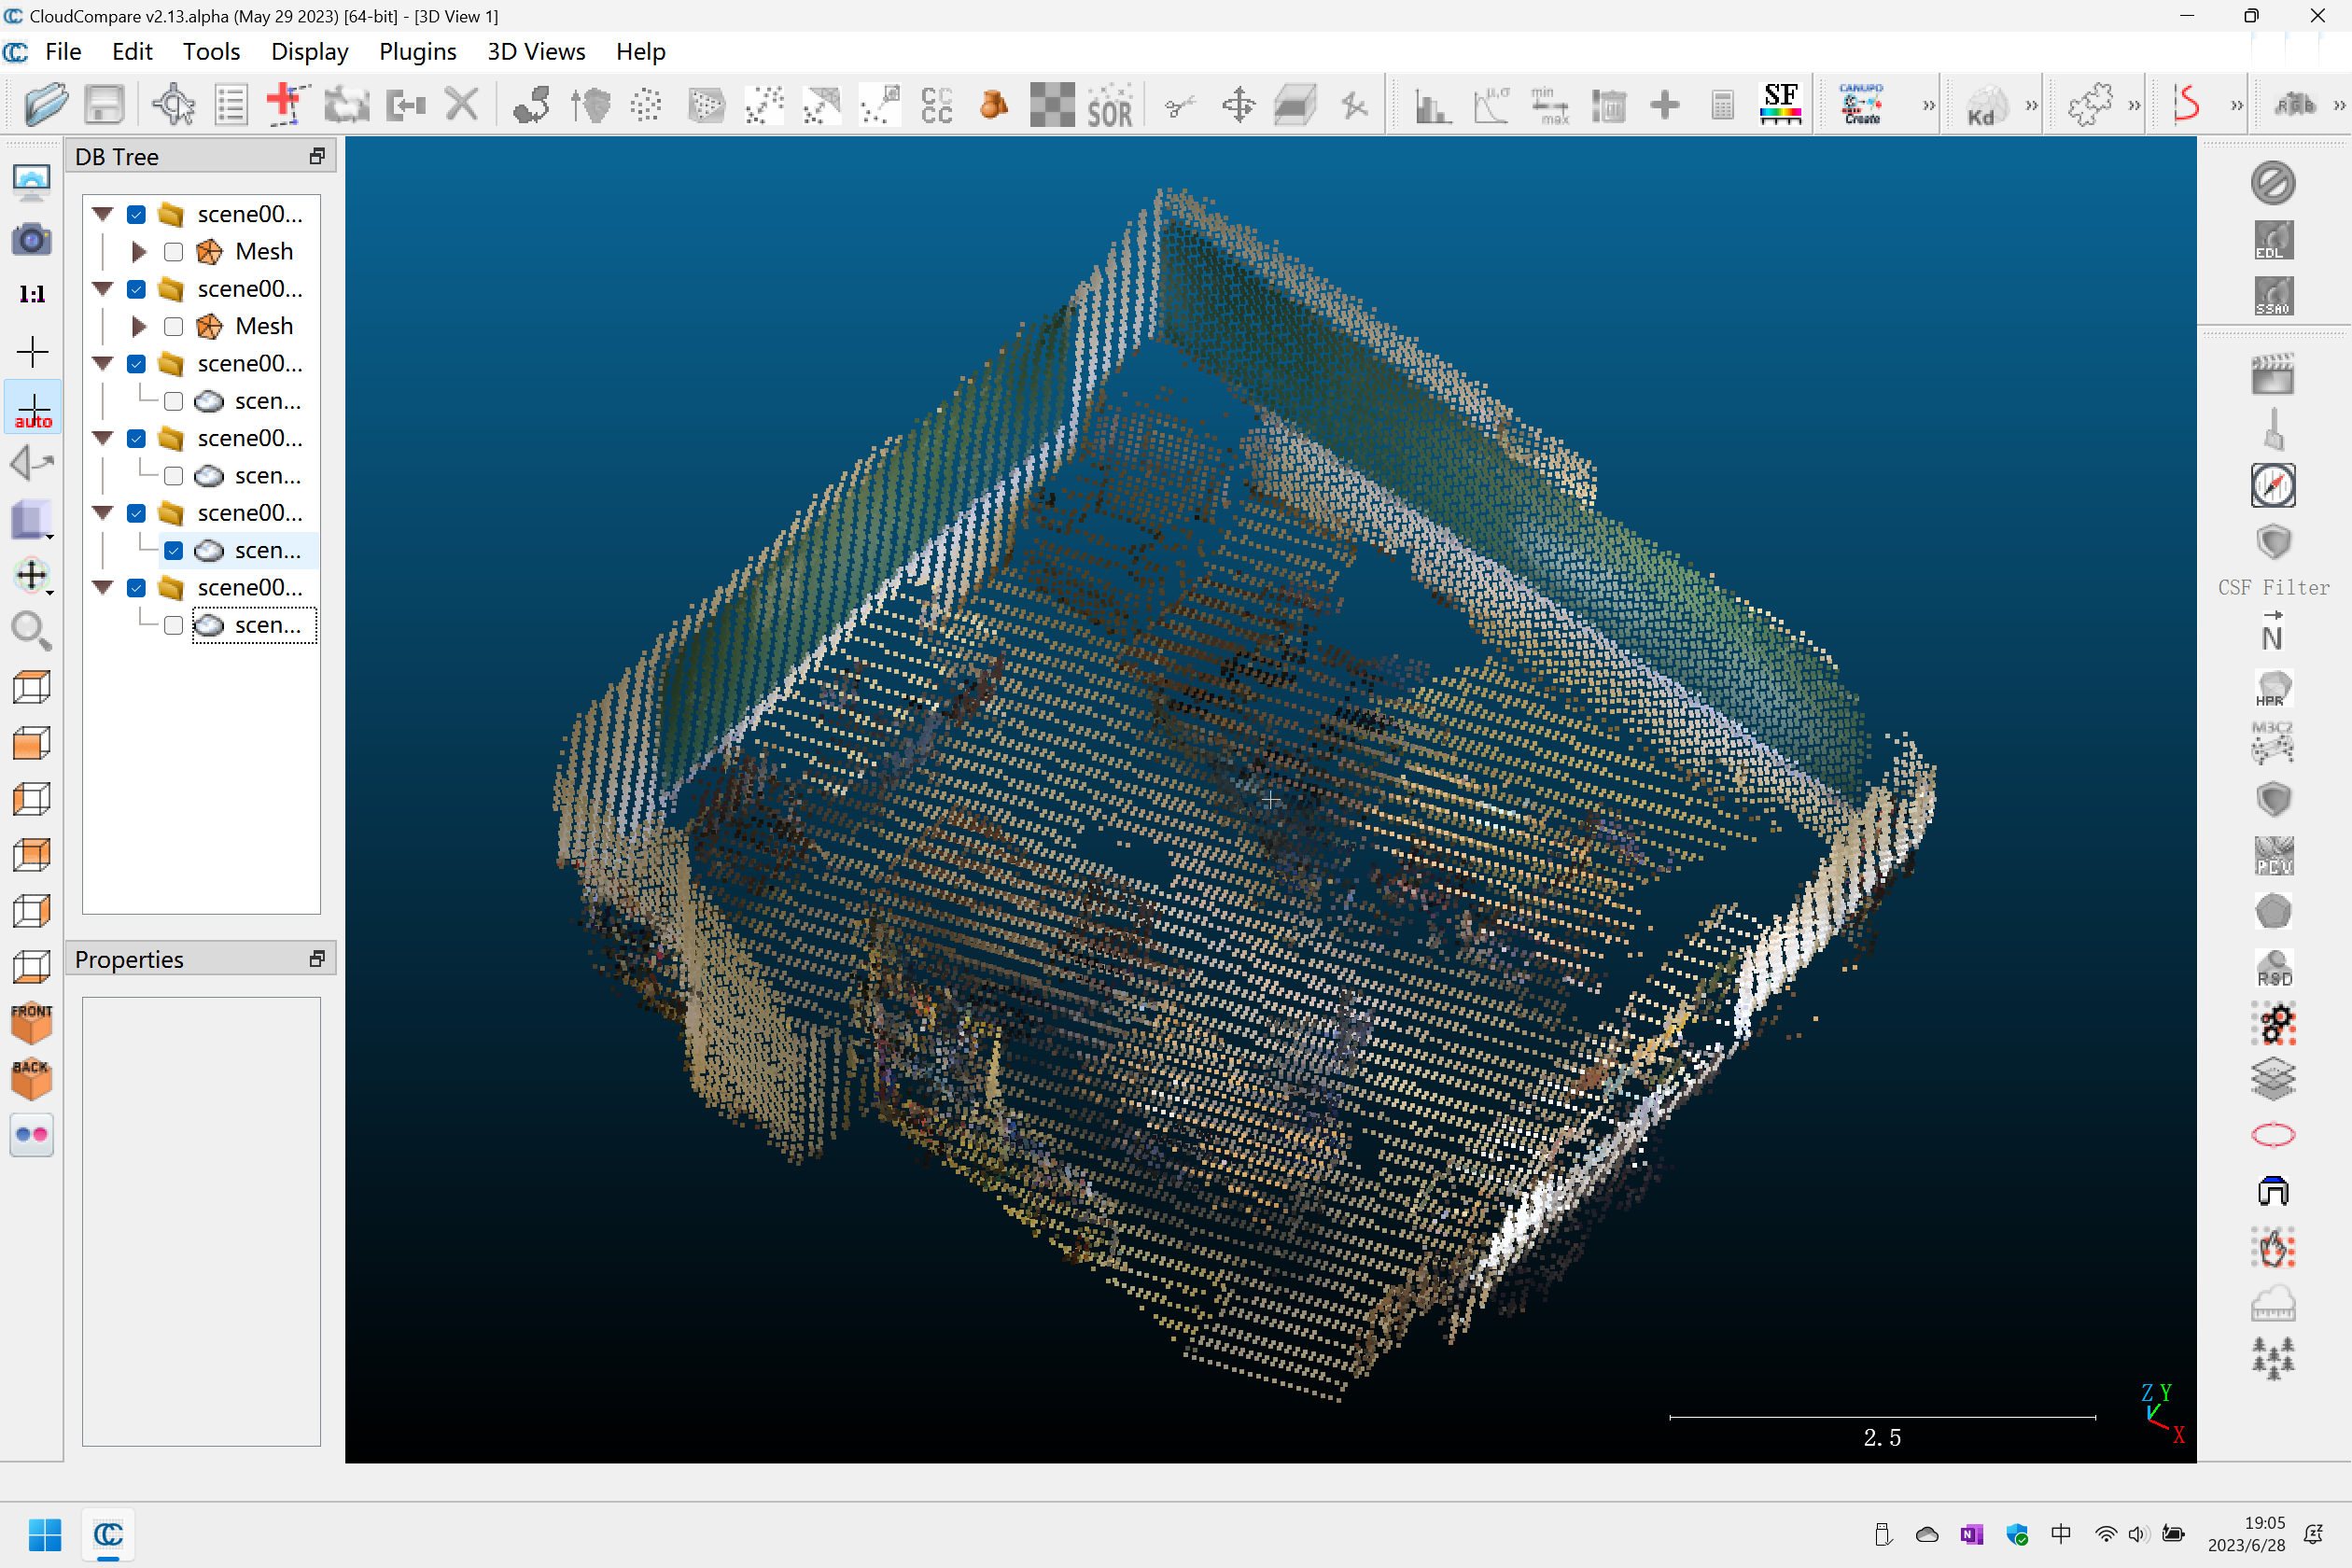
\includegraphics[width=1\textwidth]{figures/result/scene0030_rgb_5cm.png}
		\end{minipage}
	}
	\subfigure[语义信息5cm模型]{
		\begin{minipage}[t]{0.48\linewidth}
			\centering
			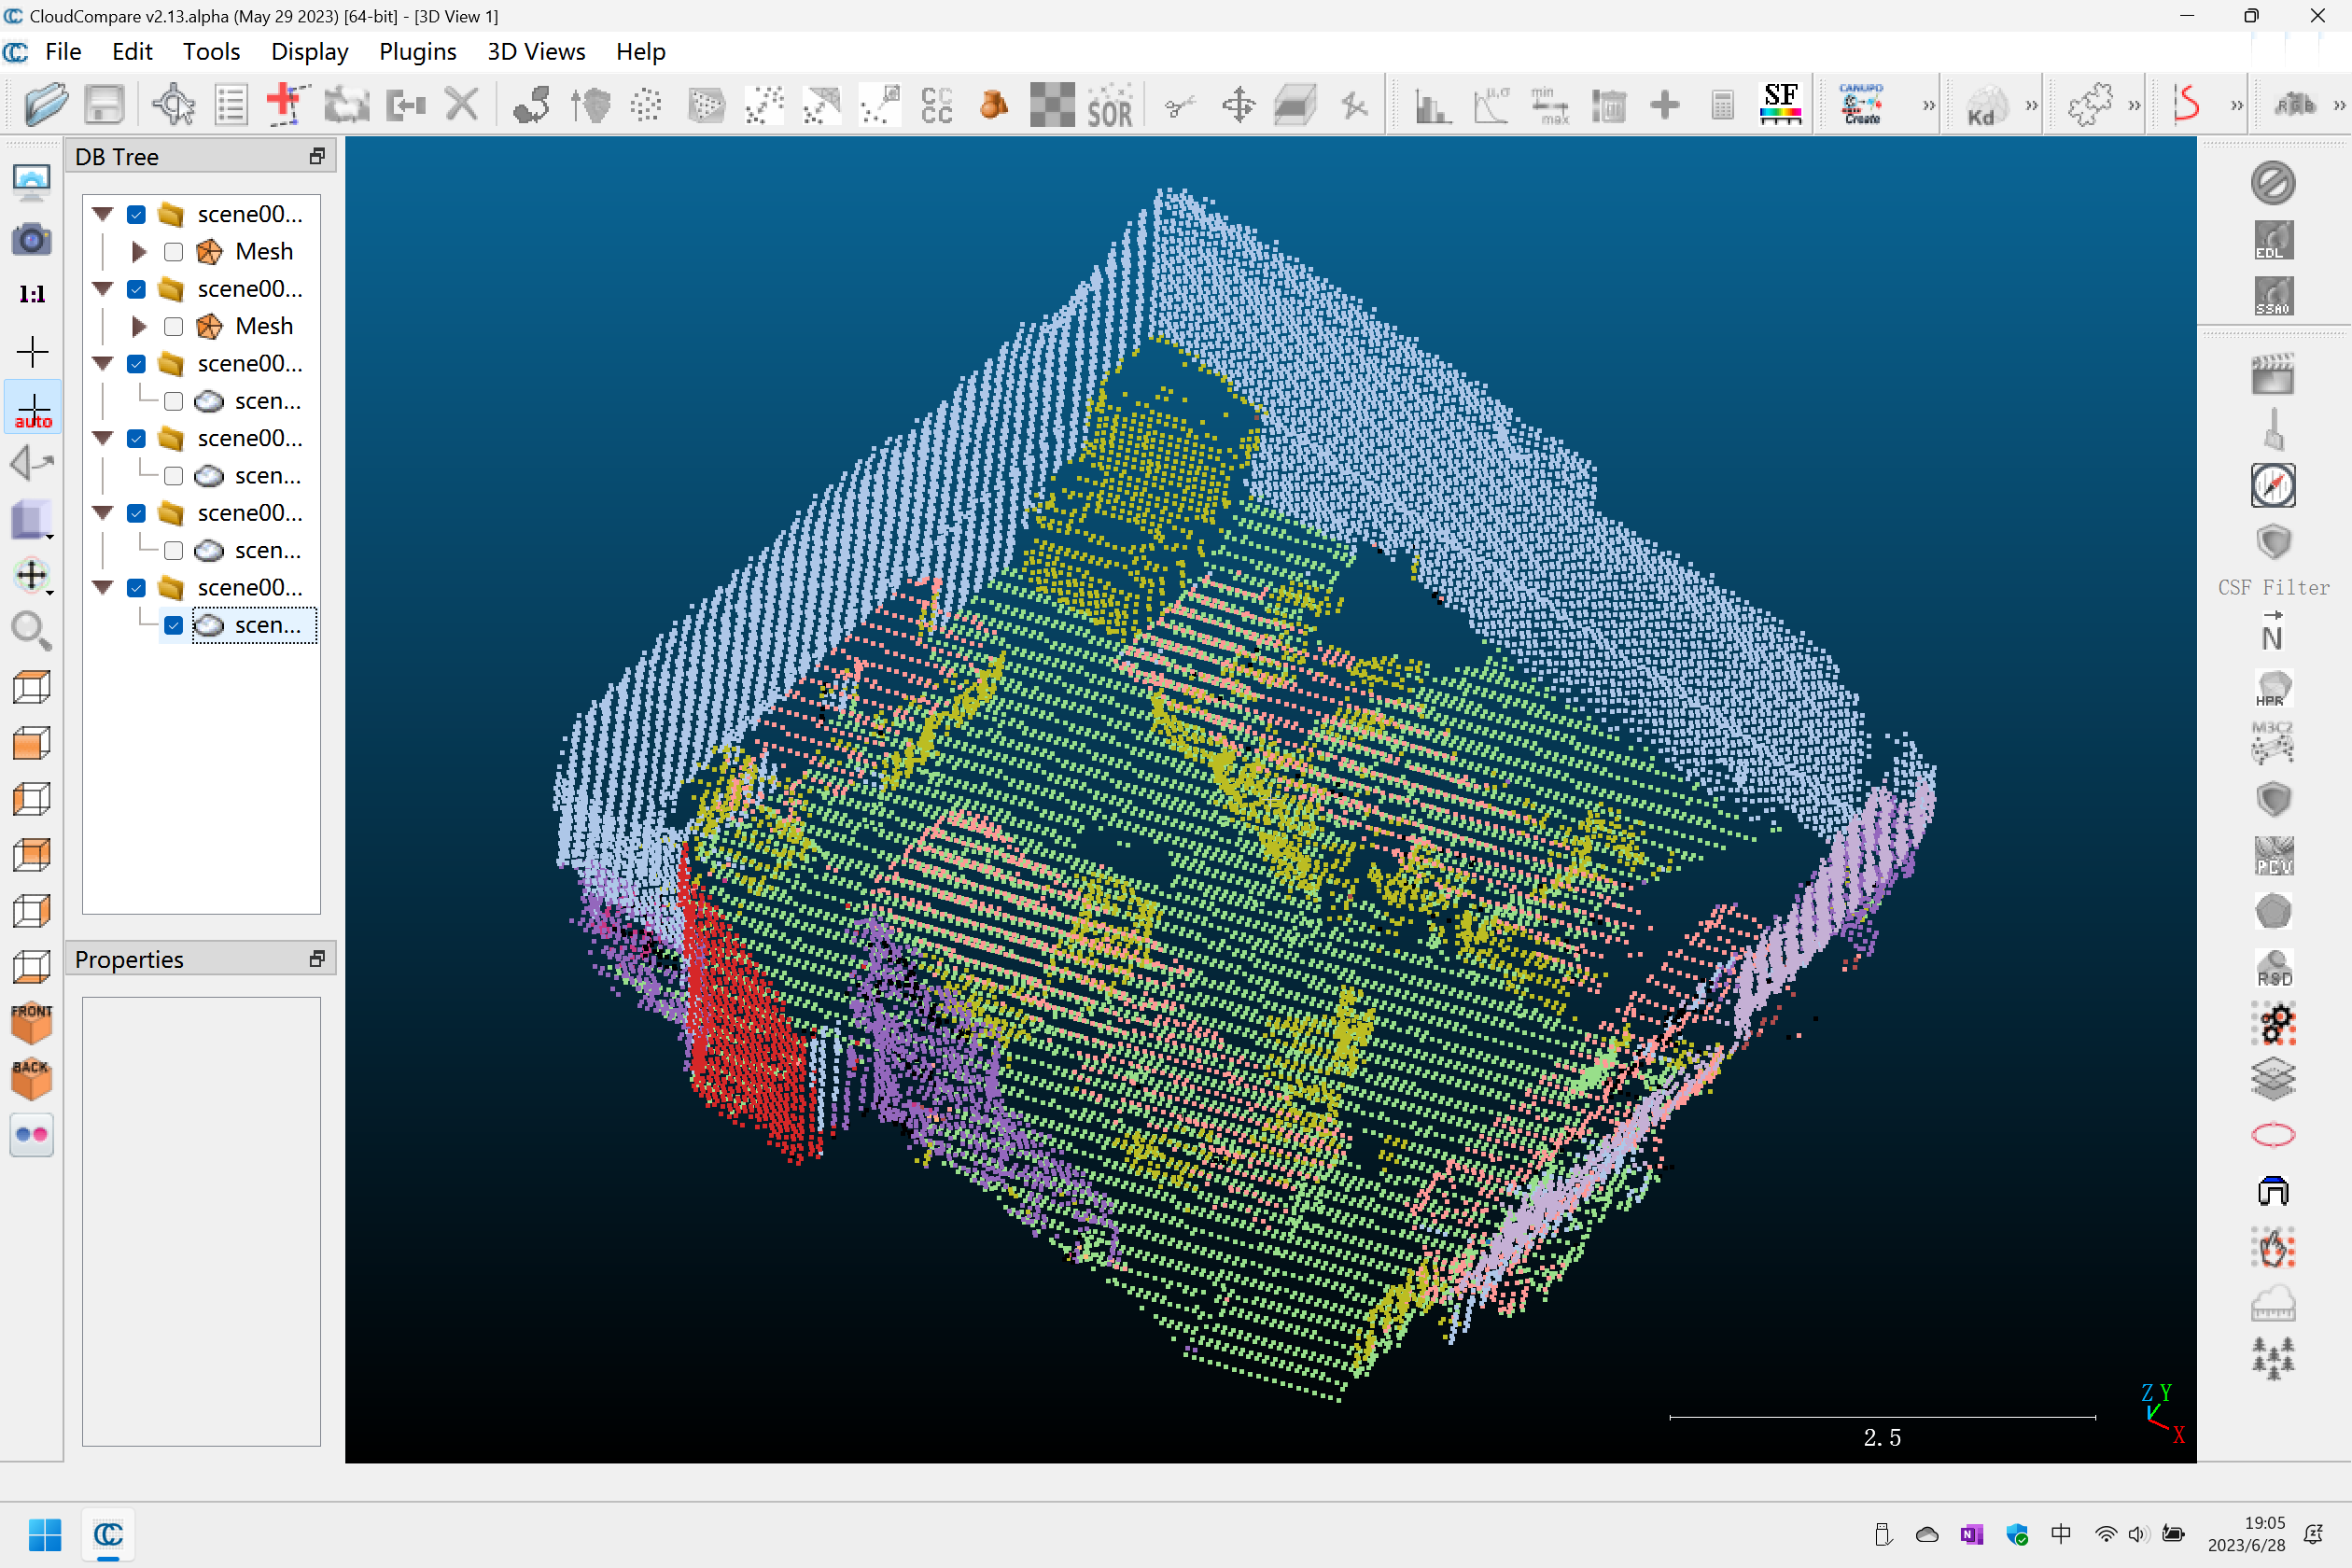
\includegraphics[width=1\textwidth]{figures/result/scene0030_label_5cm.png}
		\end{minipage}
	}
	\caption{场景scene0030\_00导出结果}
	\label{fig:scene0030_00_result}
\end{figure}

\begin{figure}[htbp]
	\centering
	\subfigure[RGB信息GT模型]{
		\begin{minipage}[t]{0.48\linewidth}
			\centering
			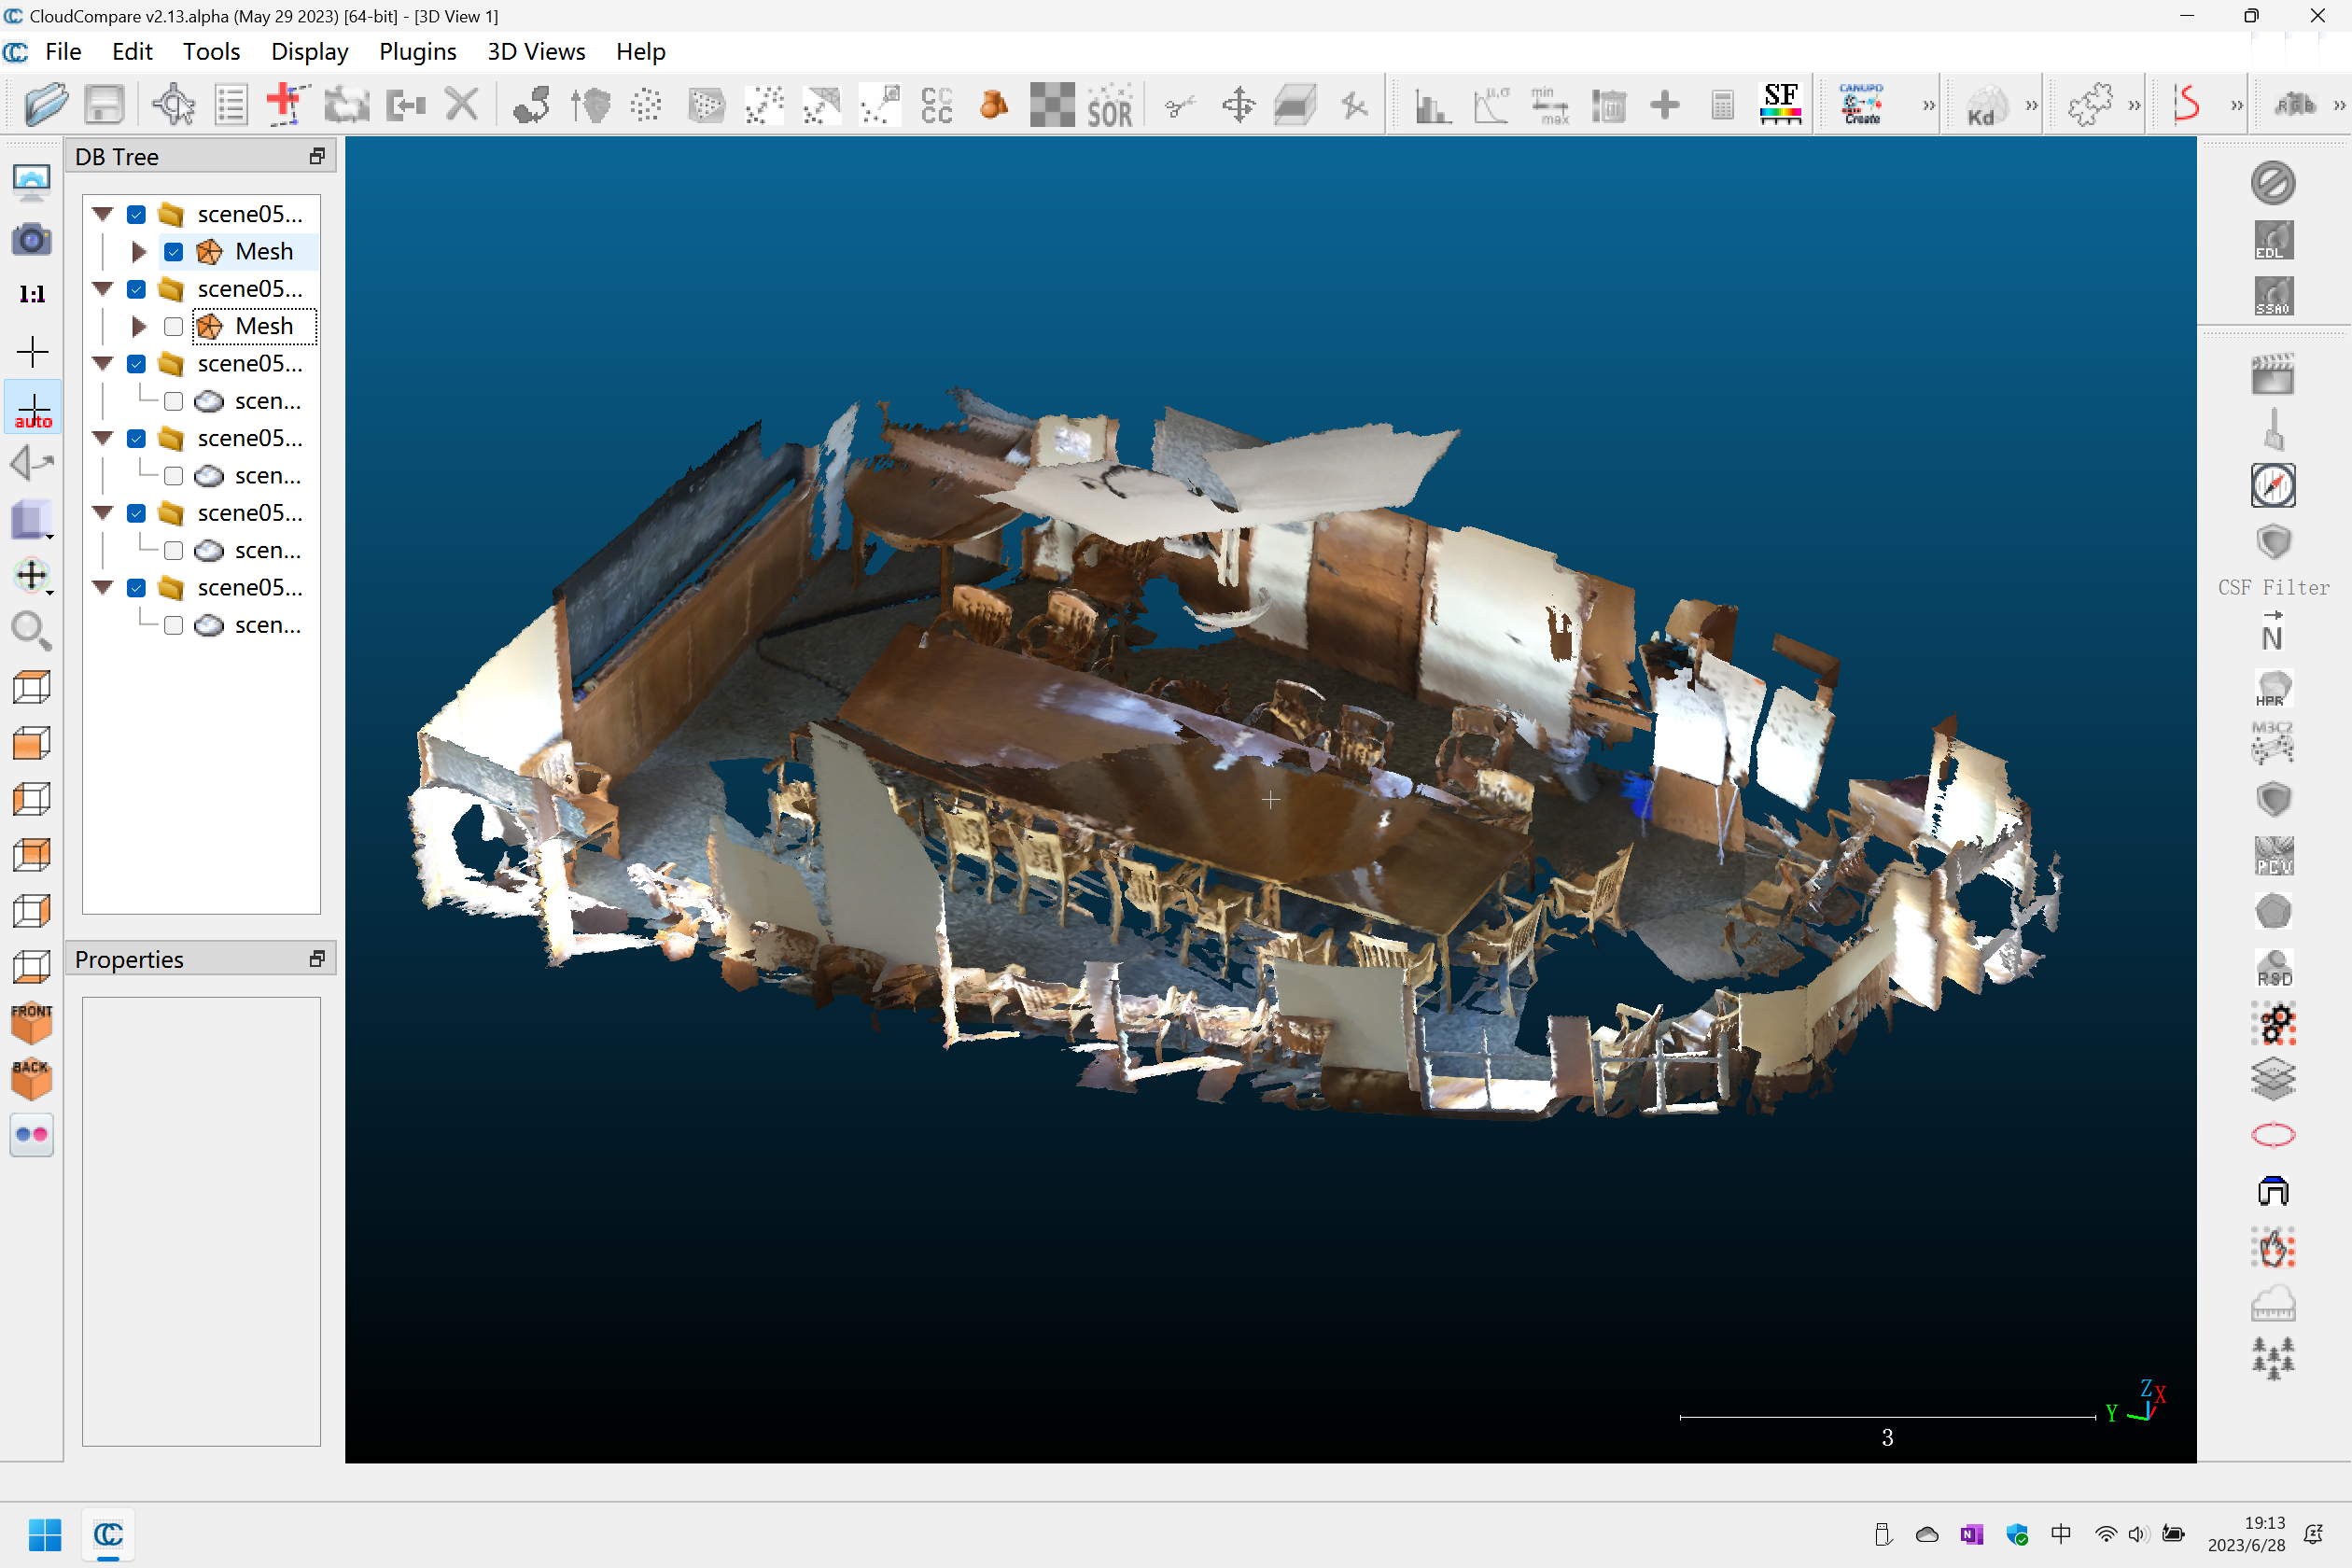
\includegraphics[width=1\textwidth]{figures/result/scene0500_rgb_gt.png}
		\end{minipage}
	}
	\subfigure[语义信息GT模型]{
		\begin{minipage}[t]{0.48\linewidth}
			\centering
			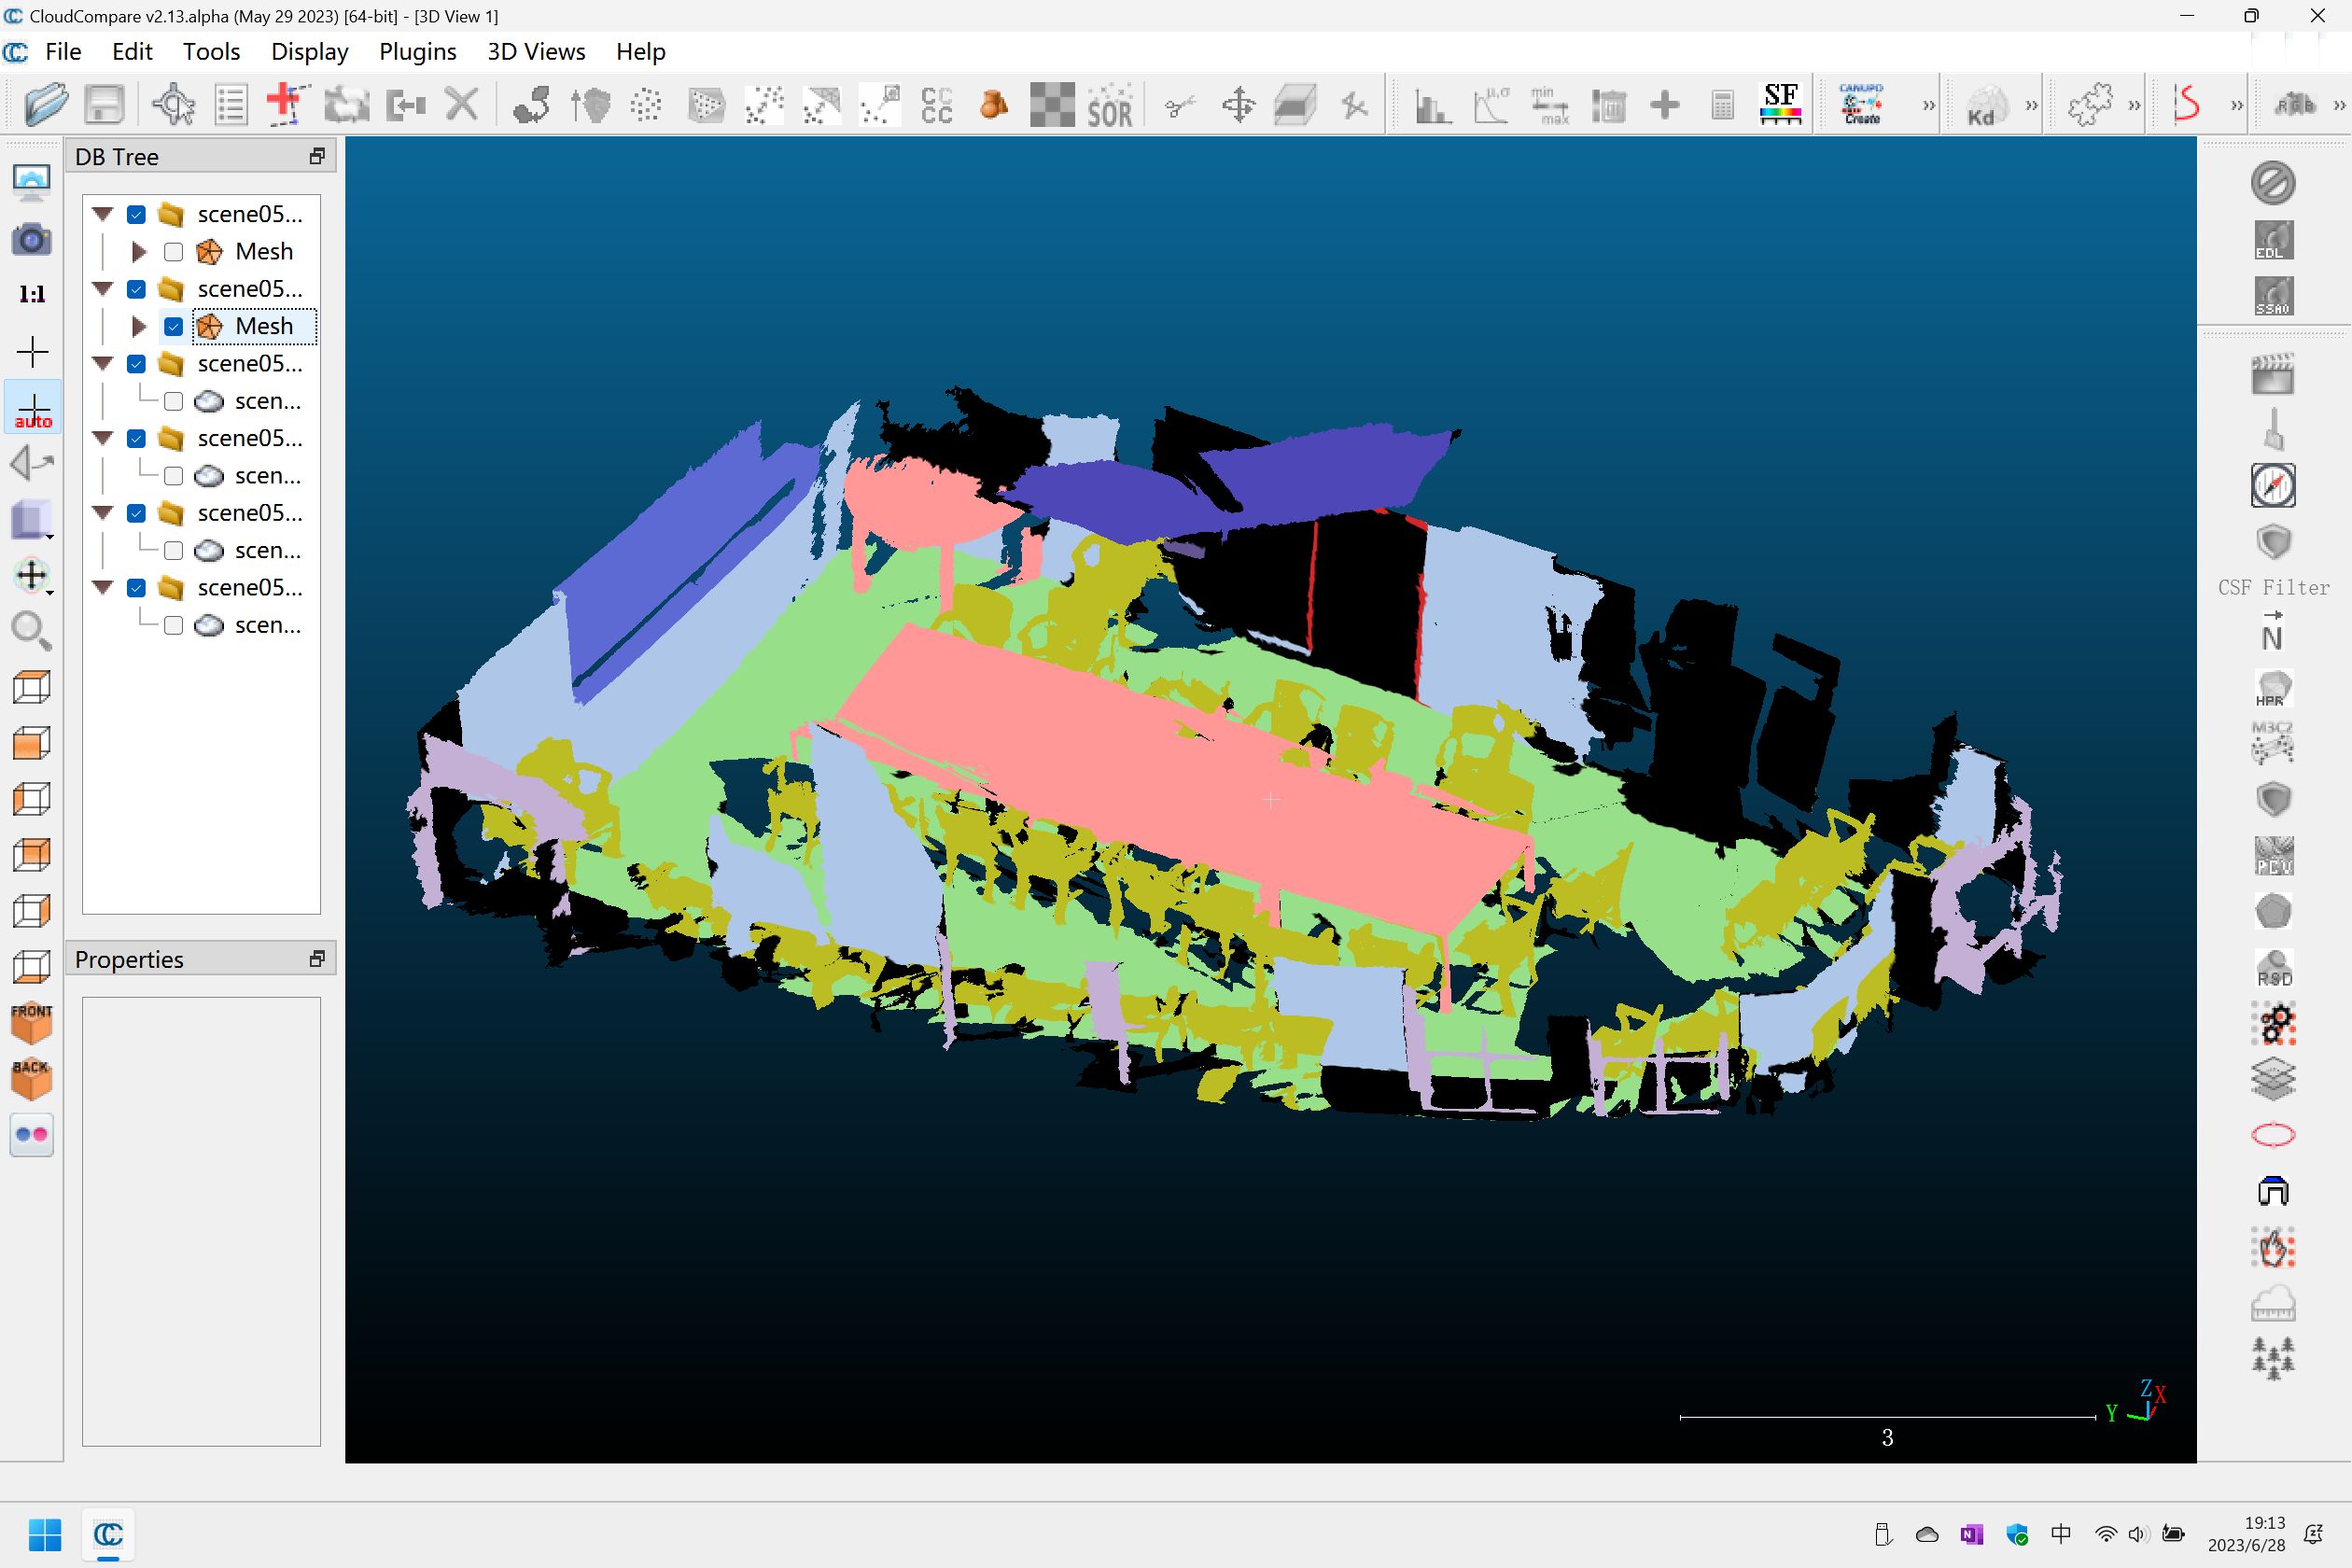
\includegraphics[width=1\textwidth]{figures/result/scene0500_label_gt.png}
		\end{minipage}
	}

	\subfigure[RGB信息2cm模型]{
		\begin{minipage}[t]{0.48\linewidth}
			\centering
			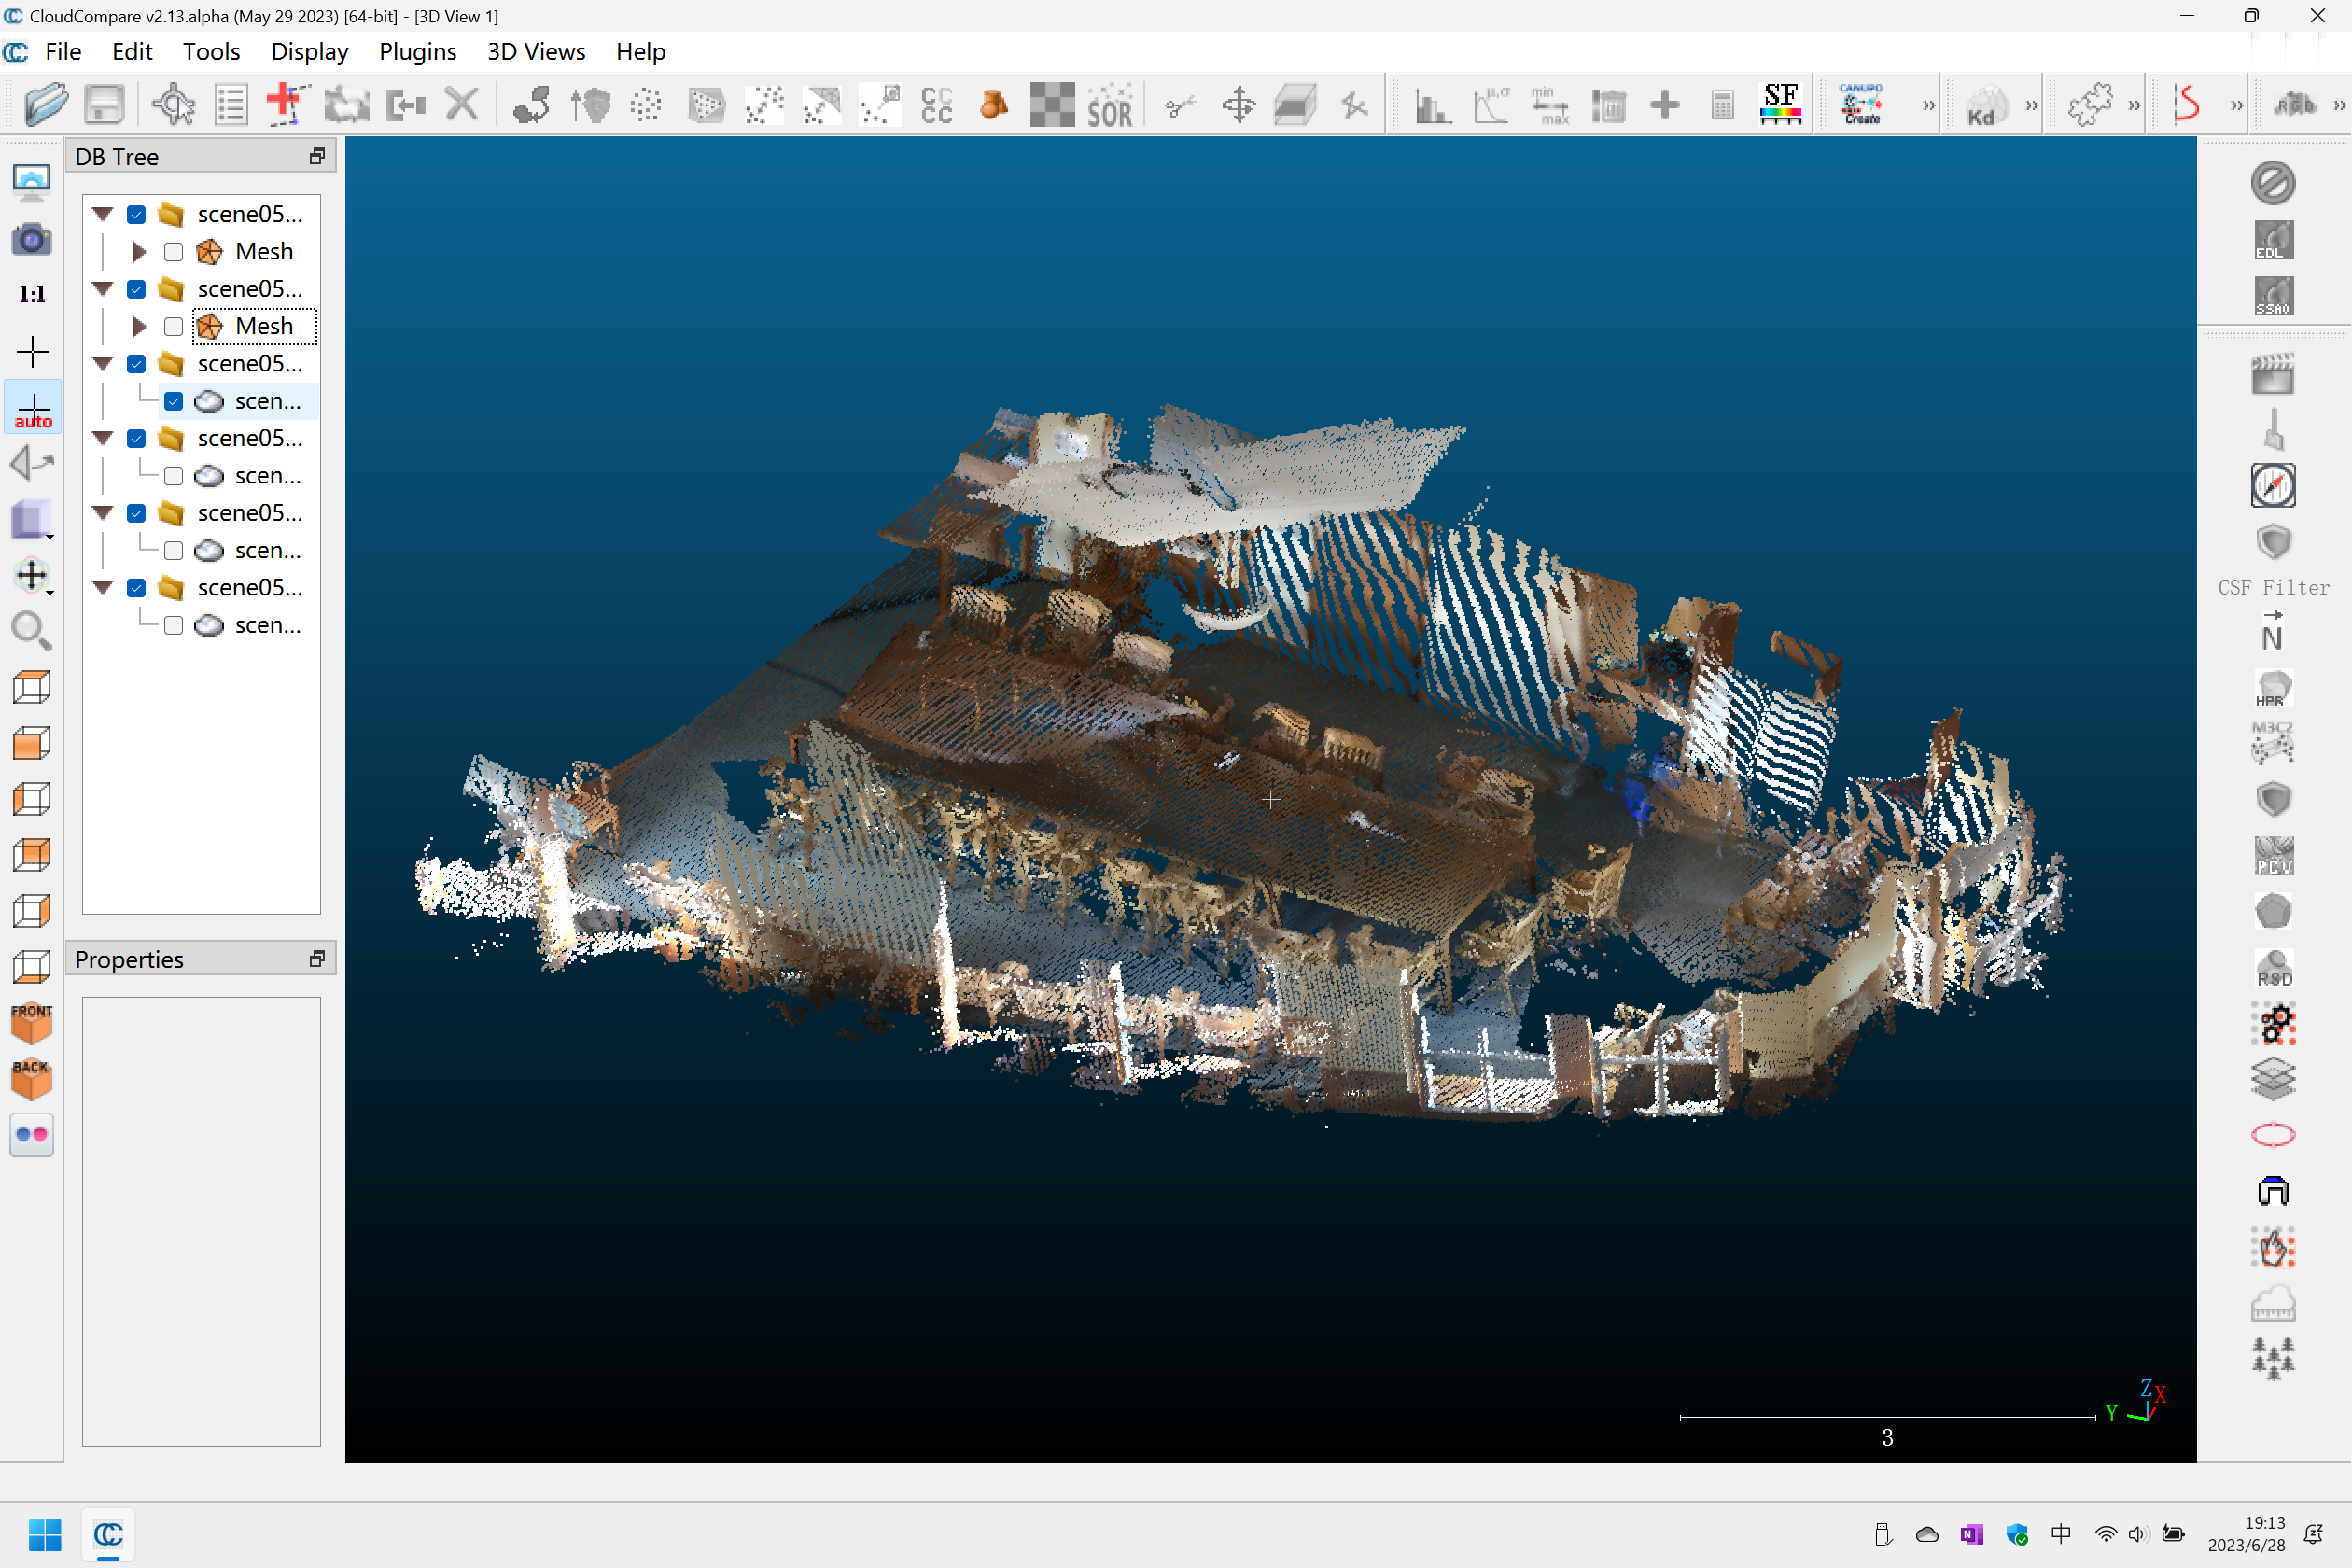
\includegraphics[width=1\textwidth]{figures/result/scene0500_rgb_2cm.png}
		\end{minipage}
	}
	\subfigure[语义信息2cm模型]{
		\begin{minipage}[t]{0.48\linewidth}
			\centering
			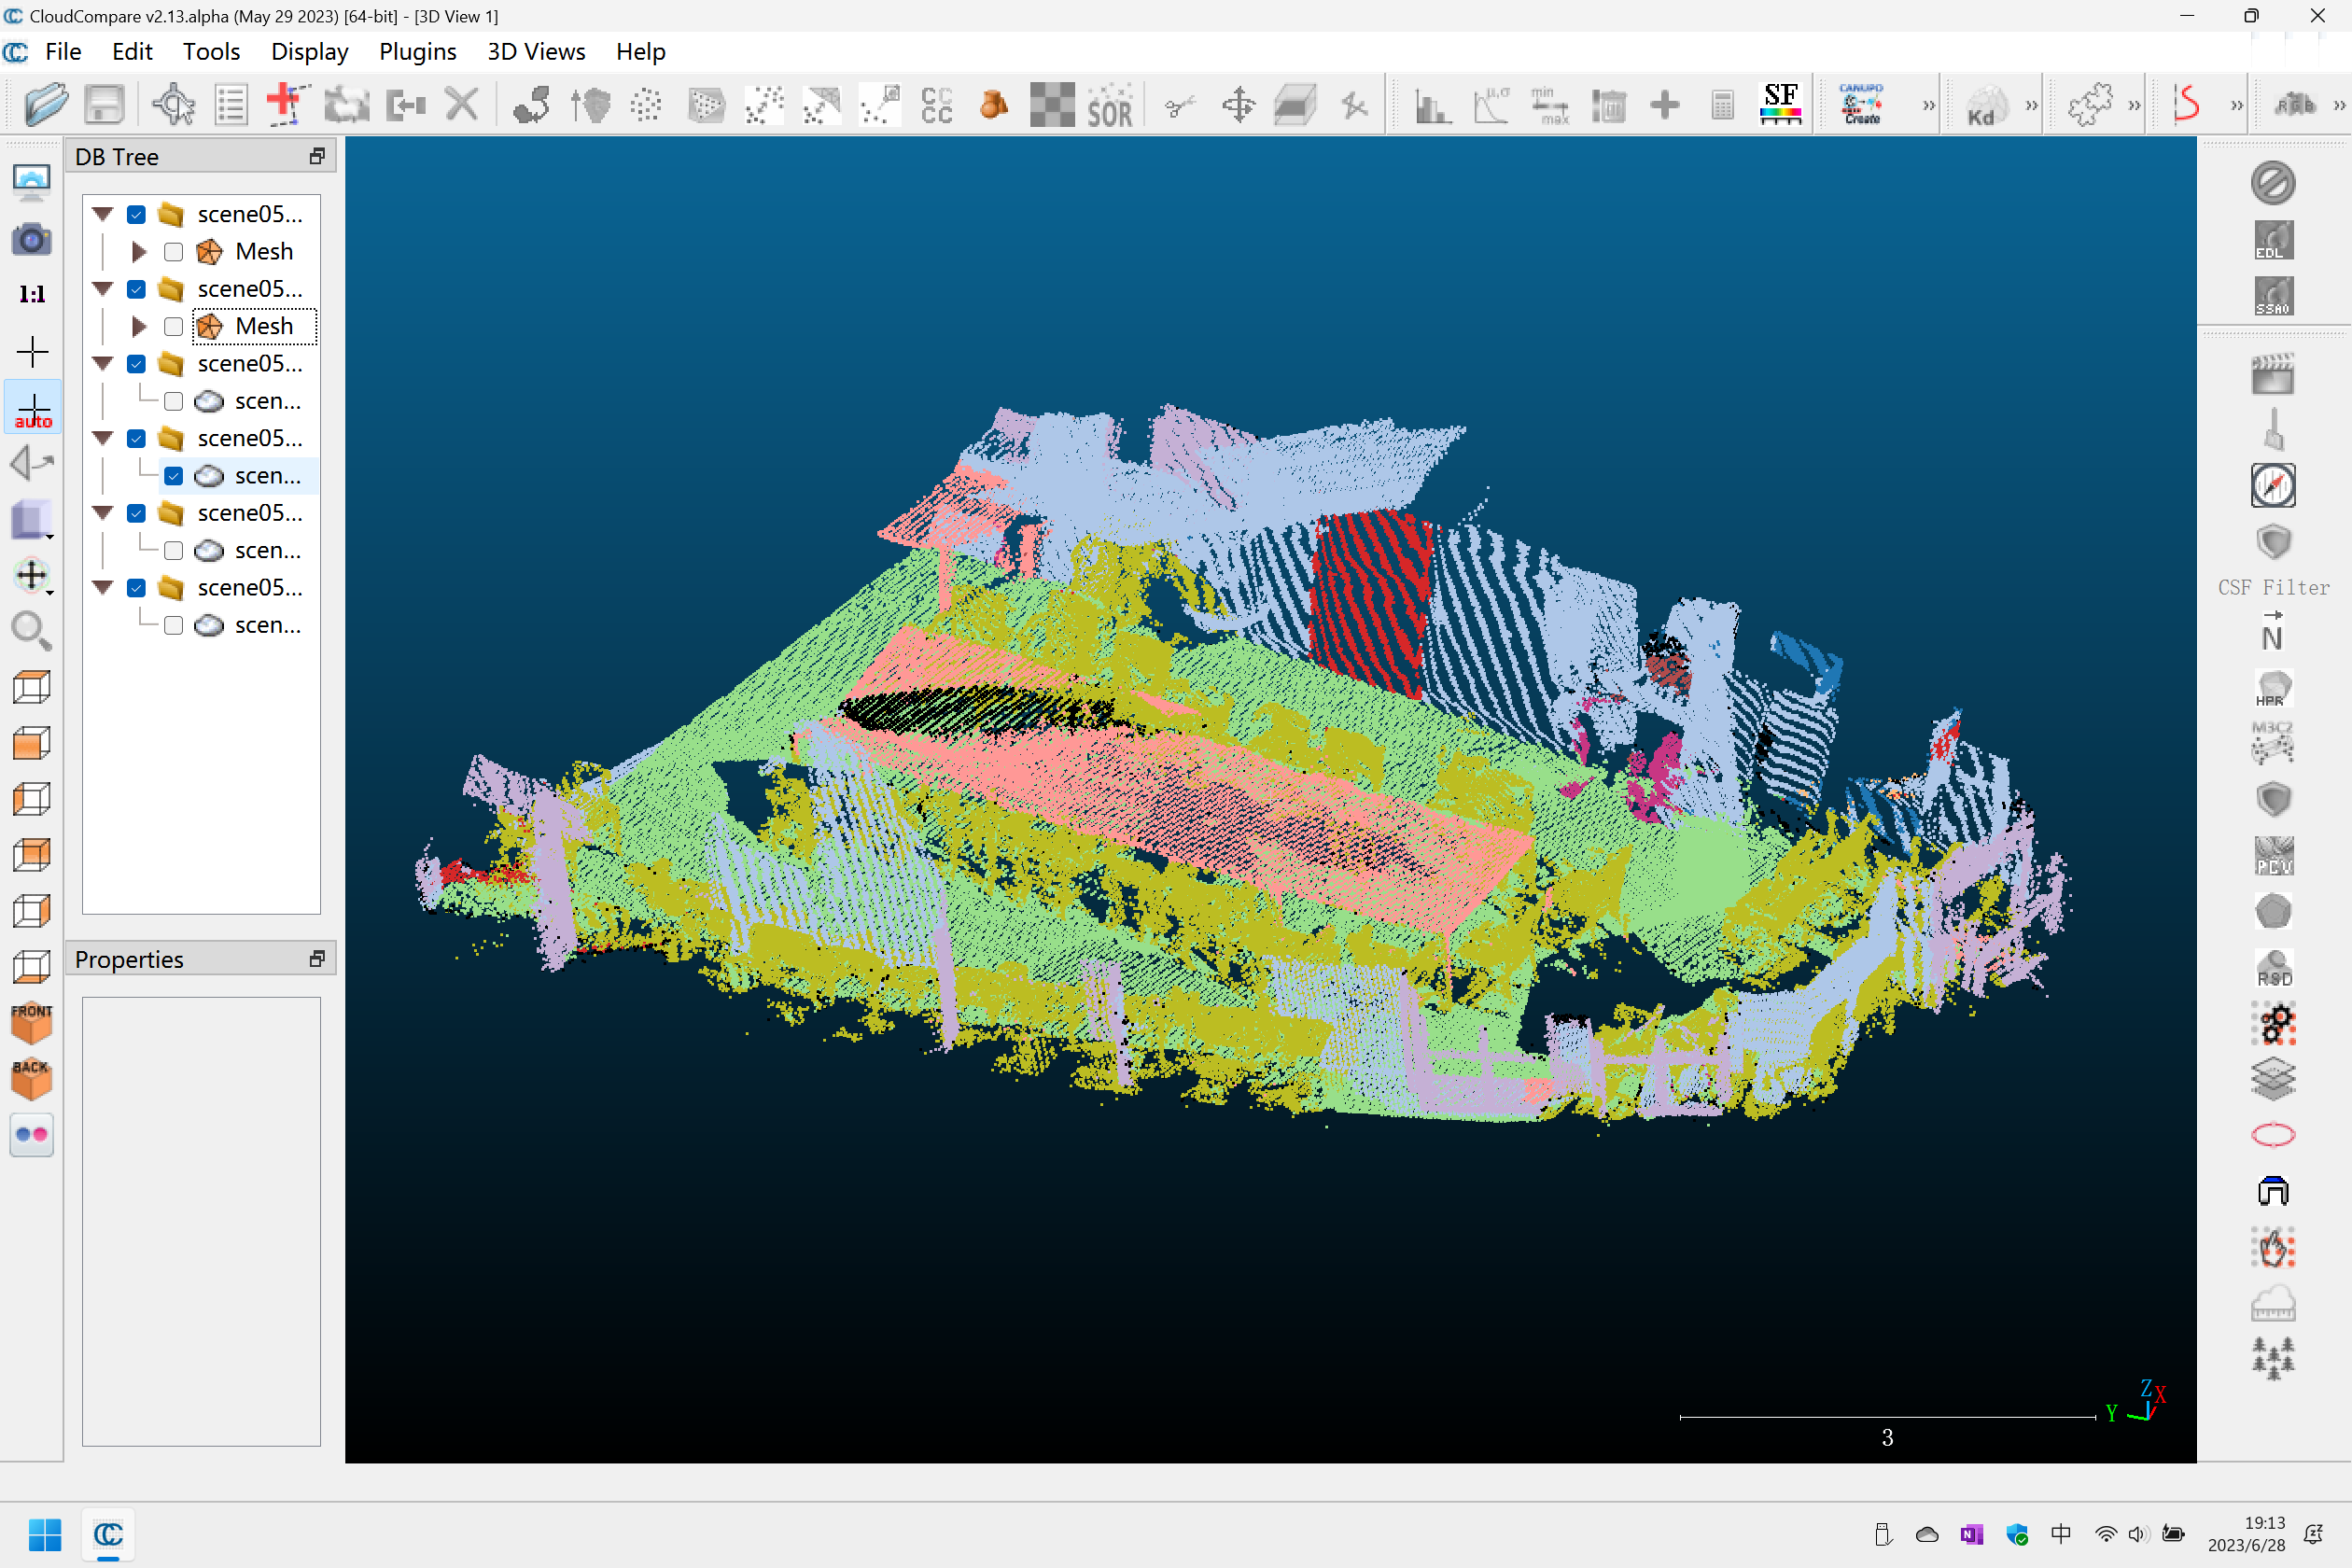
\includegraphics[width=1\textwidth]{figures/result/scene0500_label_2cm.png}
		\end{minipage}
	}

	\subfigure[RGB信息5cm模型]{
		\begin{minipage}[t]{0.48\linewidth}
			\centering
			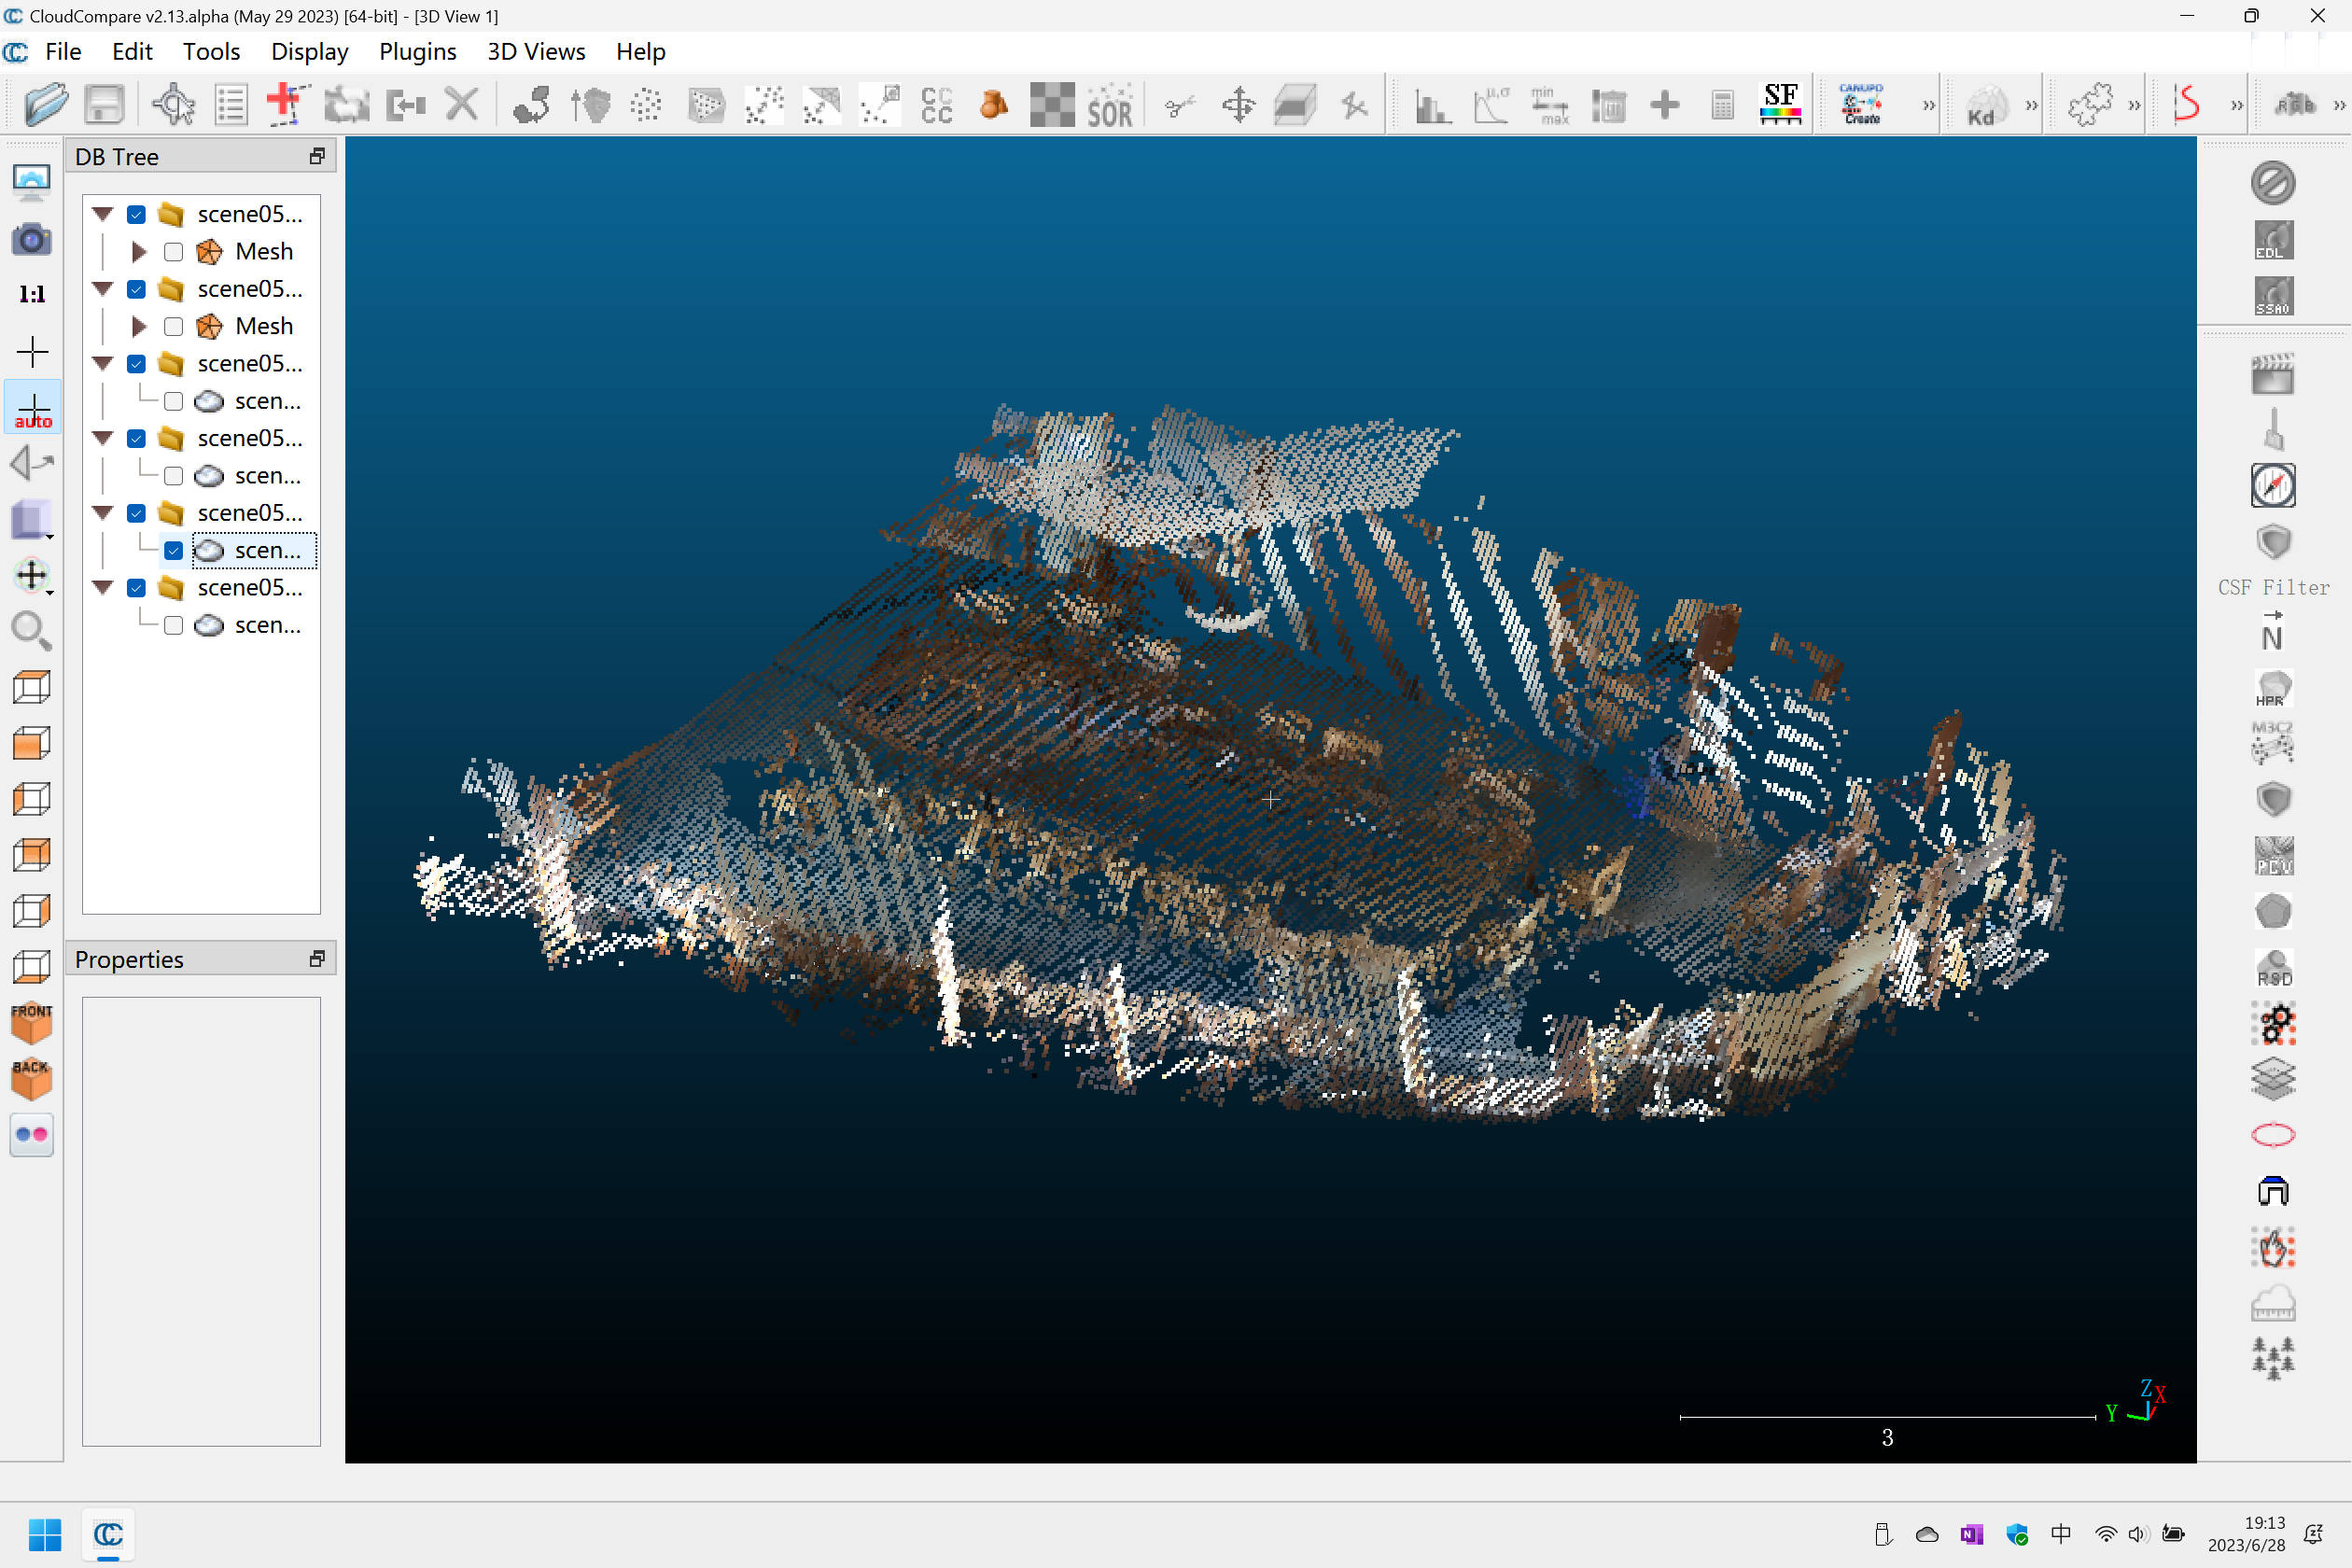
\includegraphics[width=1\textwidth]{figures/result/scene0500_rgb_5cm.png}
		\end{minipage}
	}
	\subfigure[语义信息5cm模型]{
		\begin{minipage}[t]{0.48\linewidth}
			\centering
			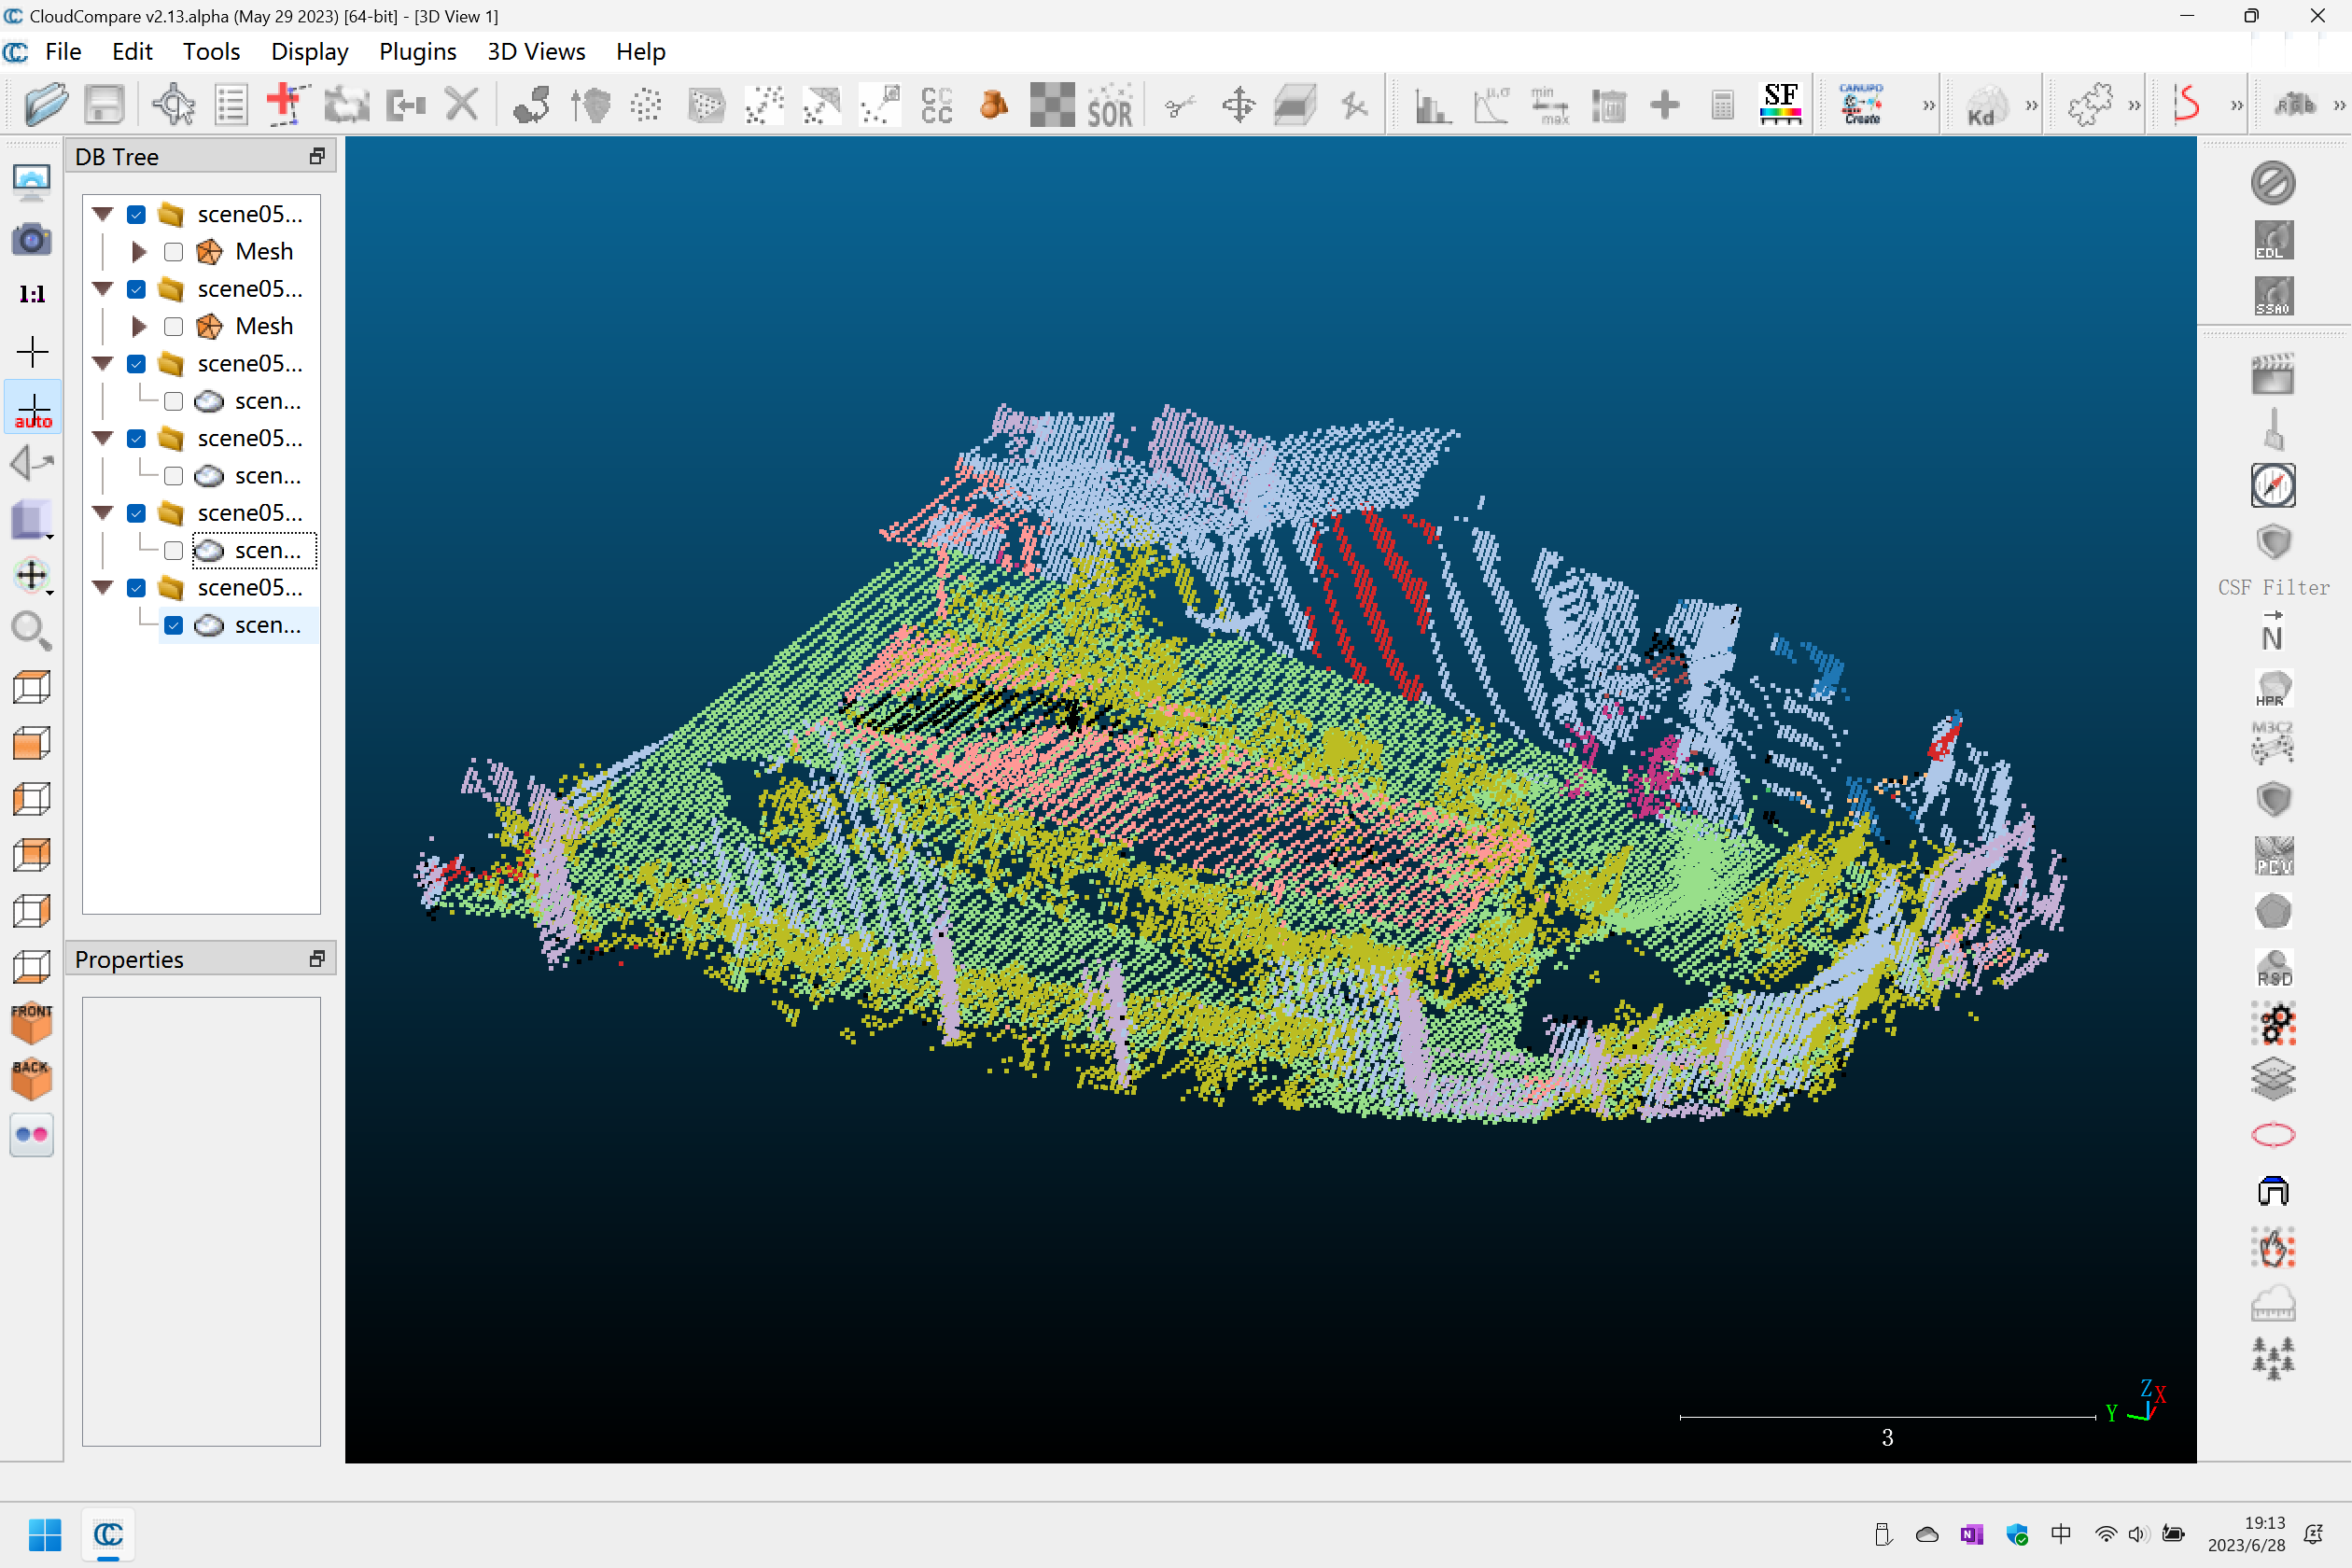
\includegraphics[width=1\textwidth]{figures/result/scene0500_label_5cm.png}
		\end{minipage}
	}
	\caption{场景scene0500\_00导出结果}
	\label{fig:scene0500_00_result}
\end{figure}

\begin{figure}
	\centering
	\subfigure[RGB信息GT模型]{
		\begin{minipage}[t]{0.48\linewidth}
			\centering
			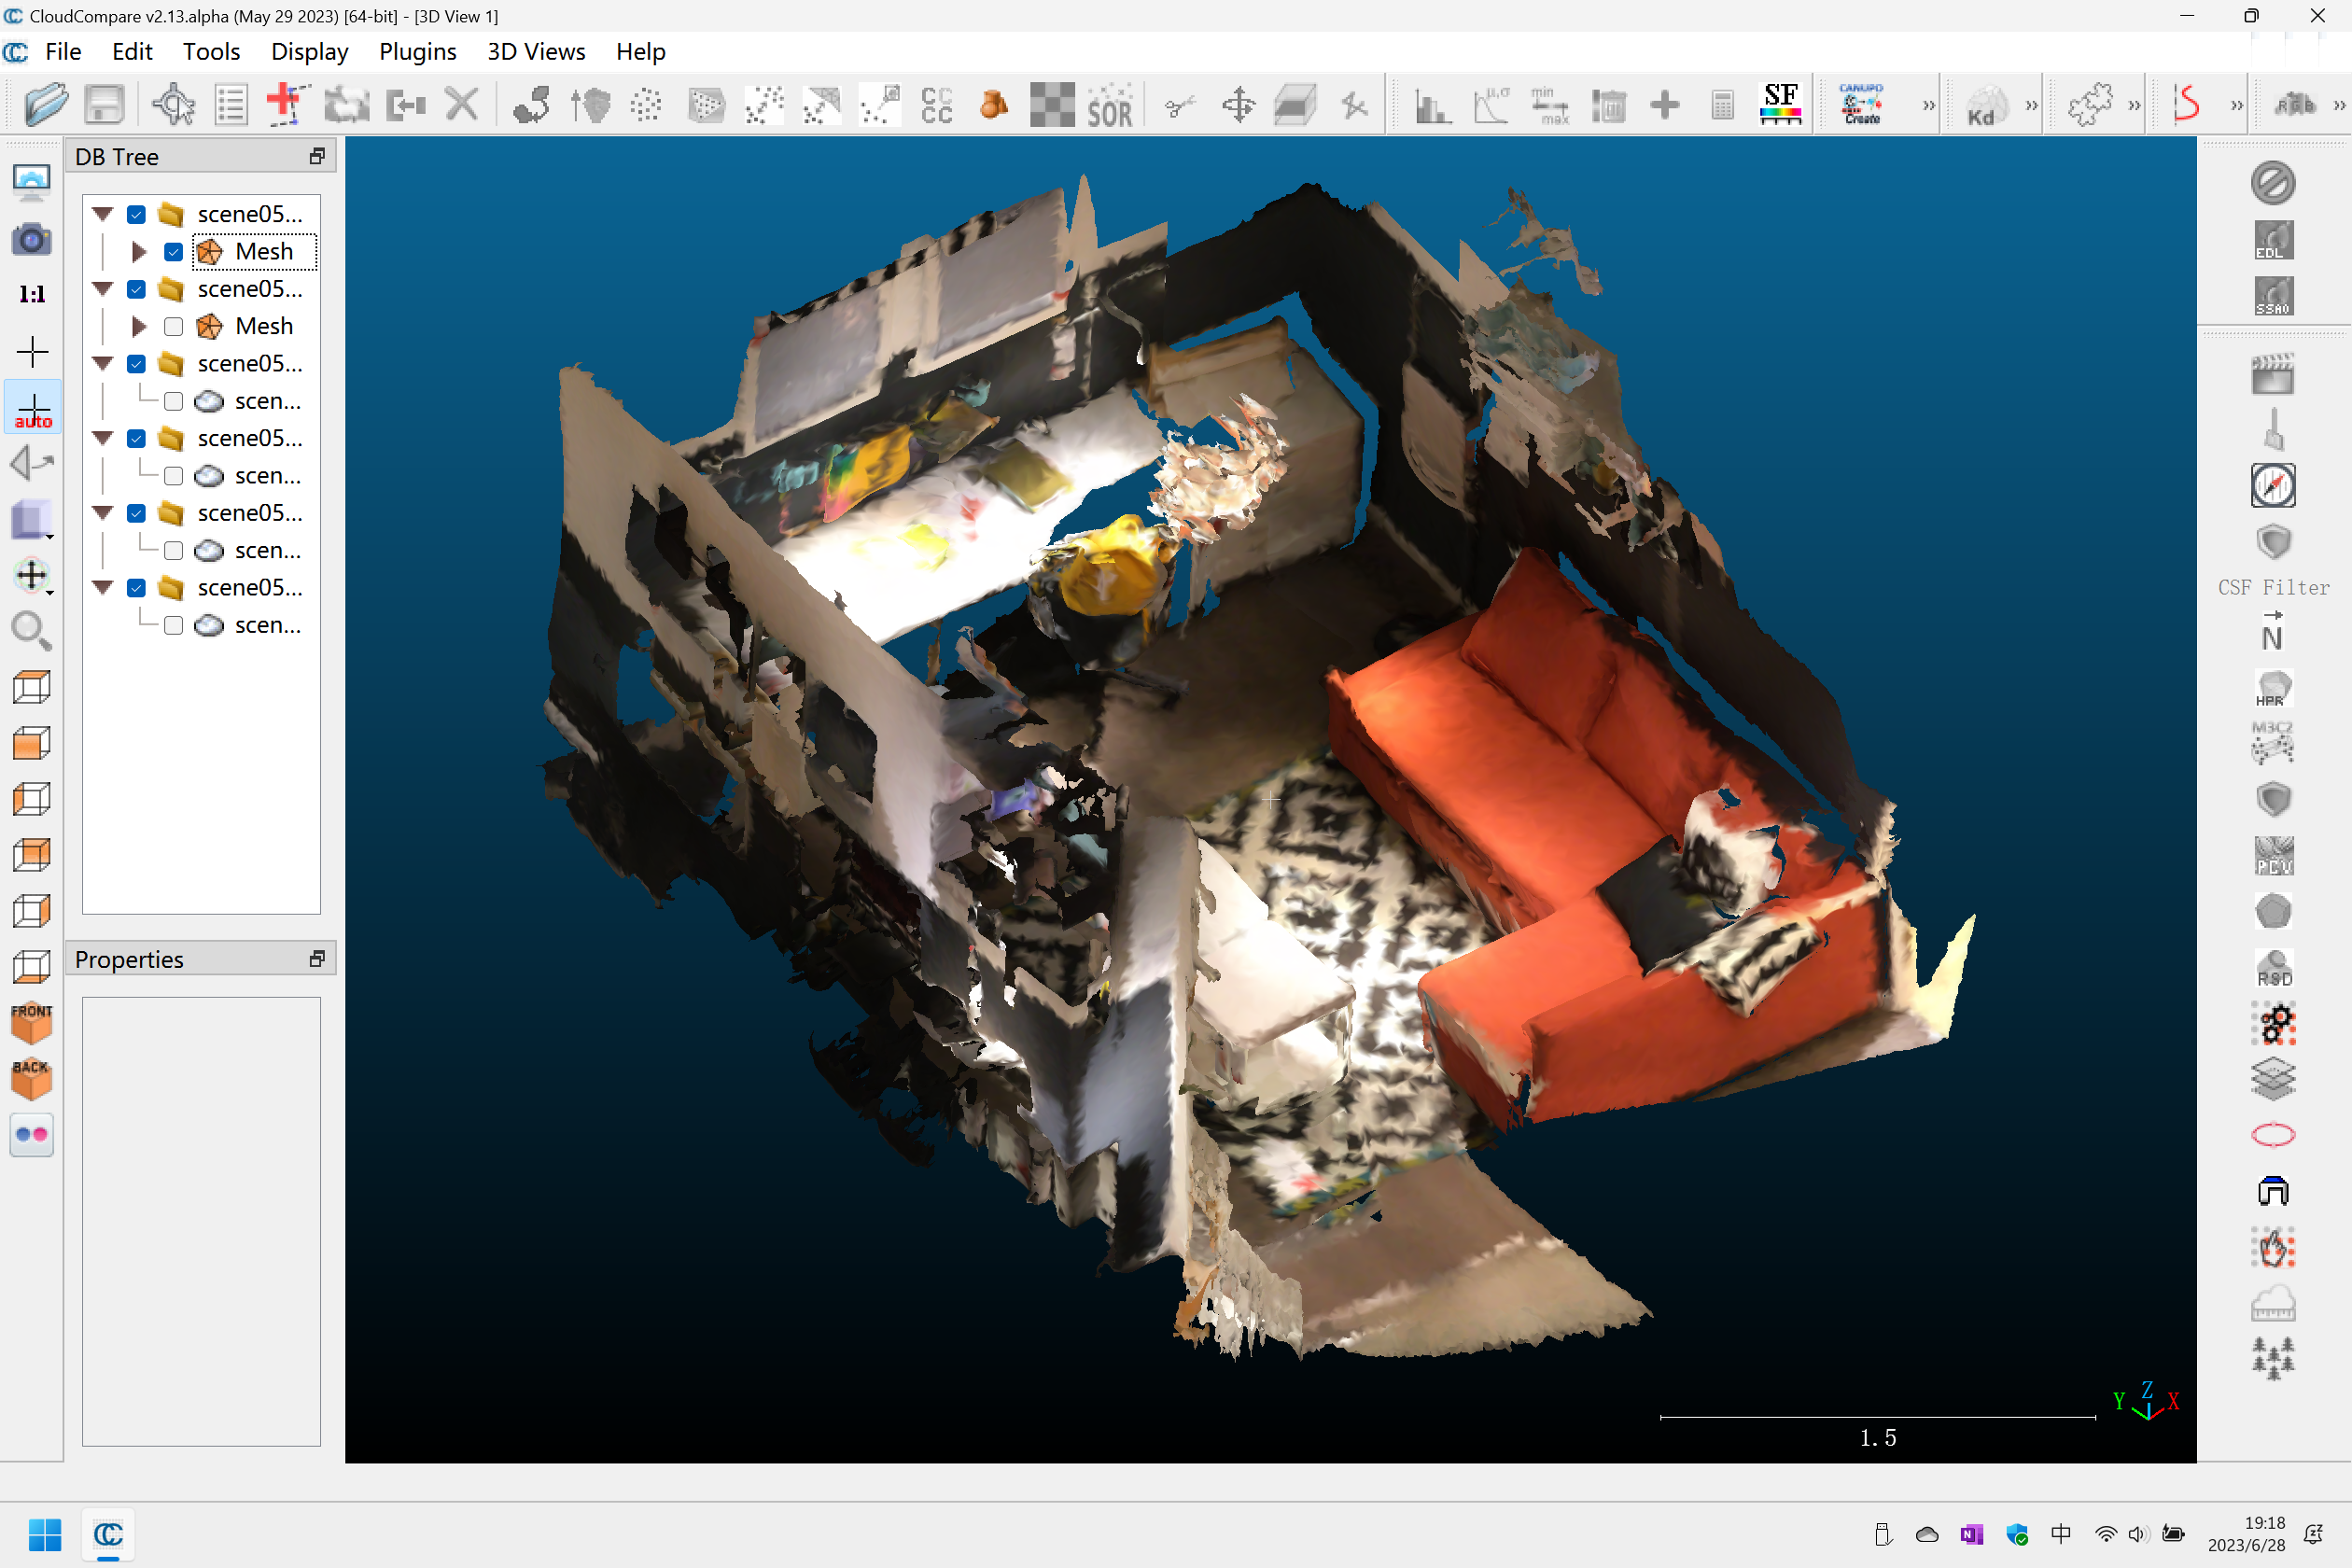
\includegraphics[width=1\textwidth]{figures/result/scene0518_rgb_gt.png}
		\end{minipage}
	}
	\subfigure[语义信息GT模型]{
		\begin{minipage}[t]{0.48\linewidth}
			\centering
			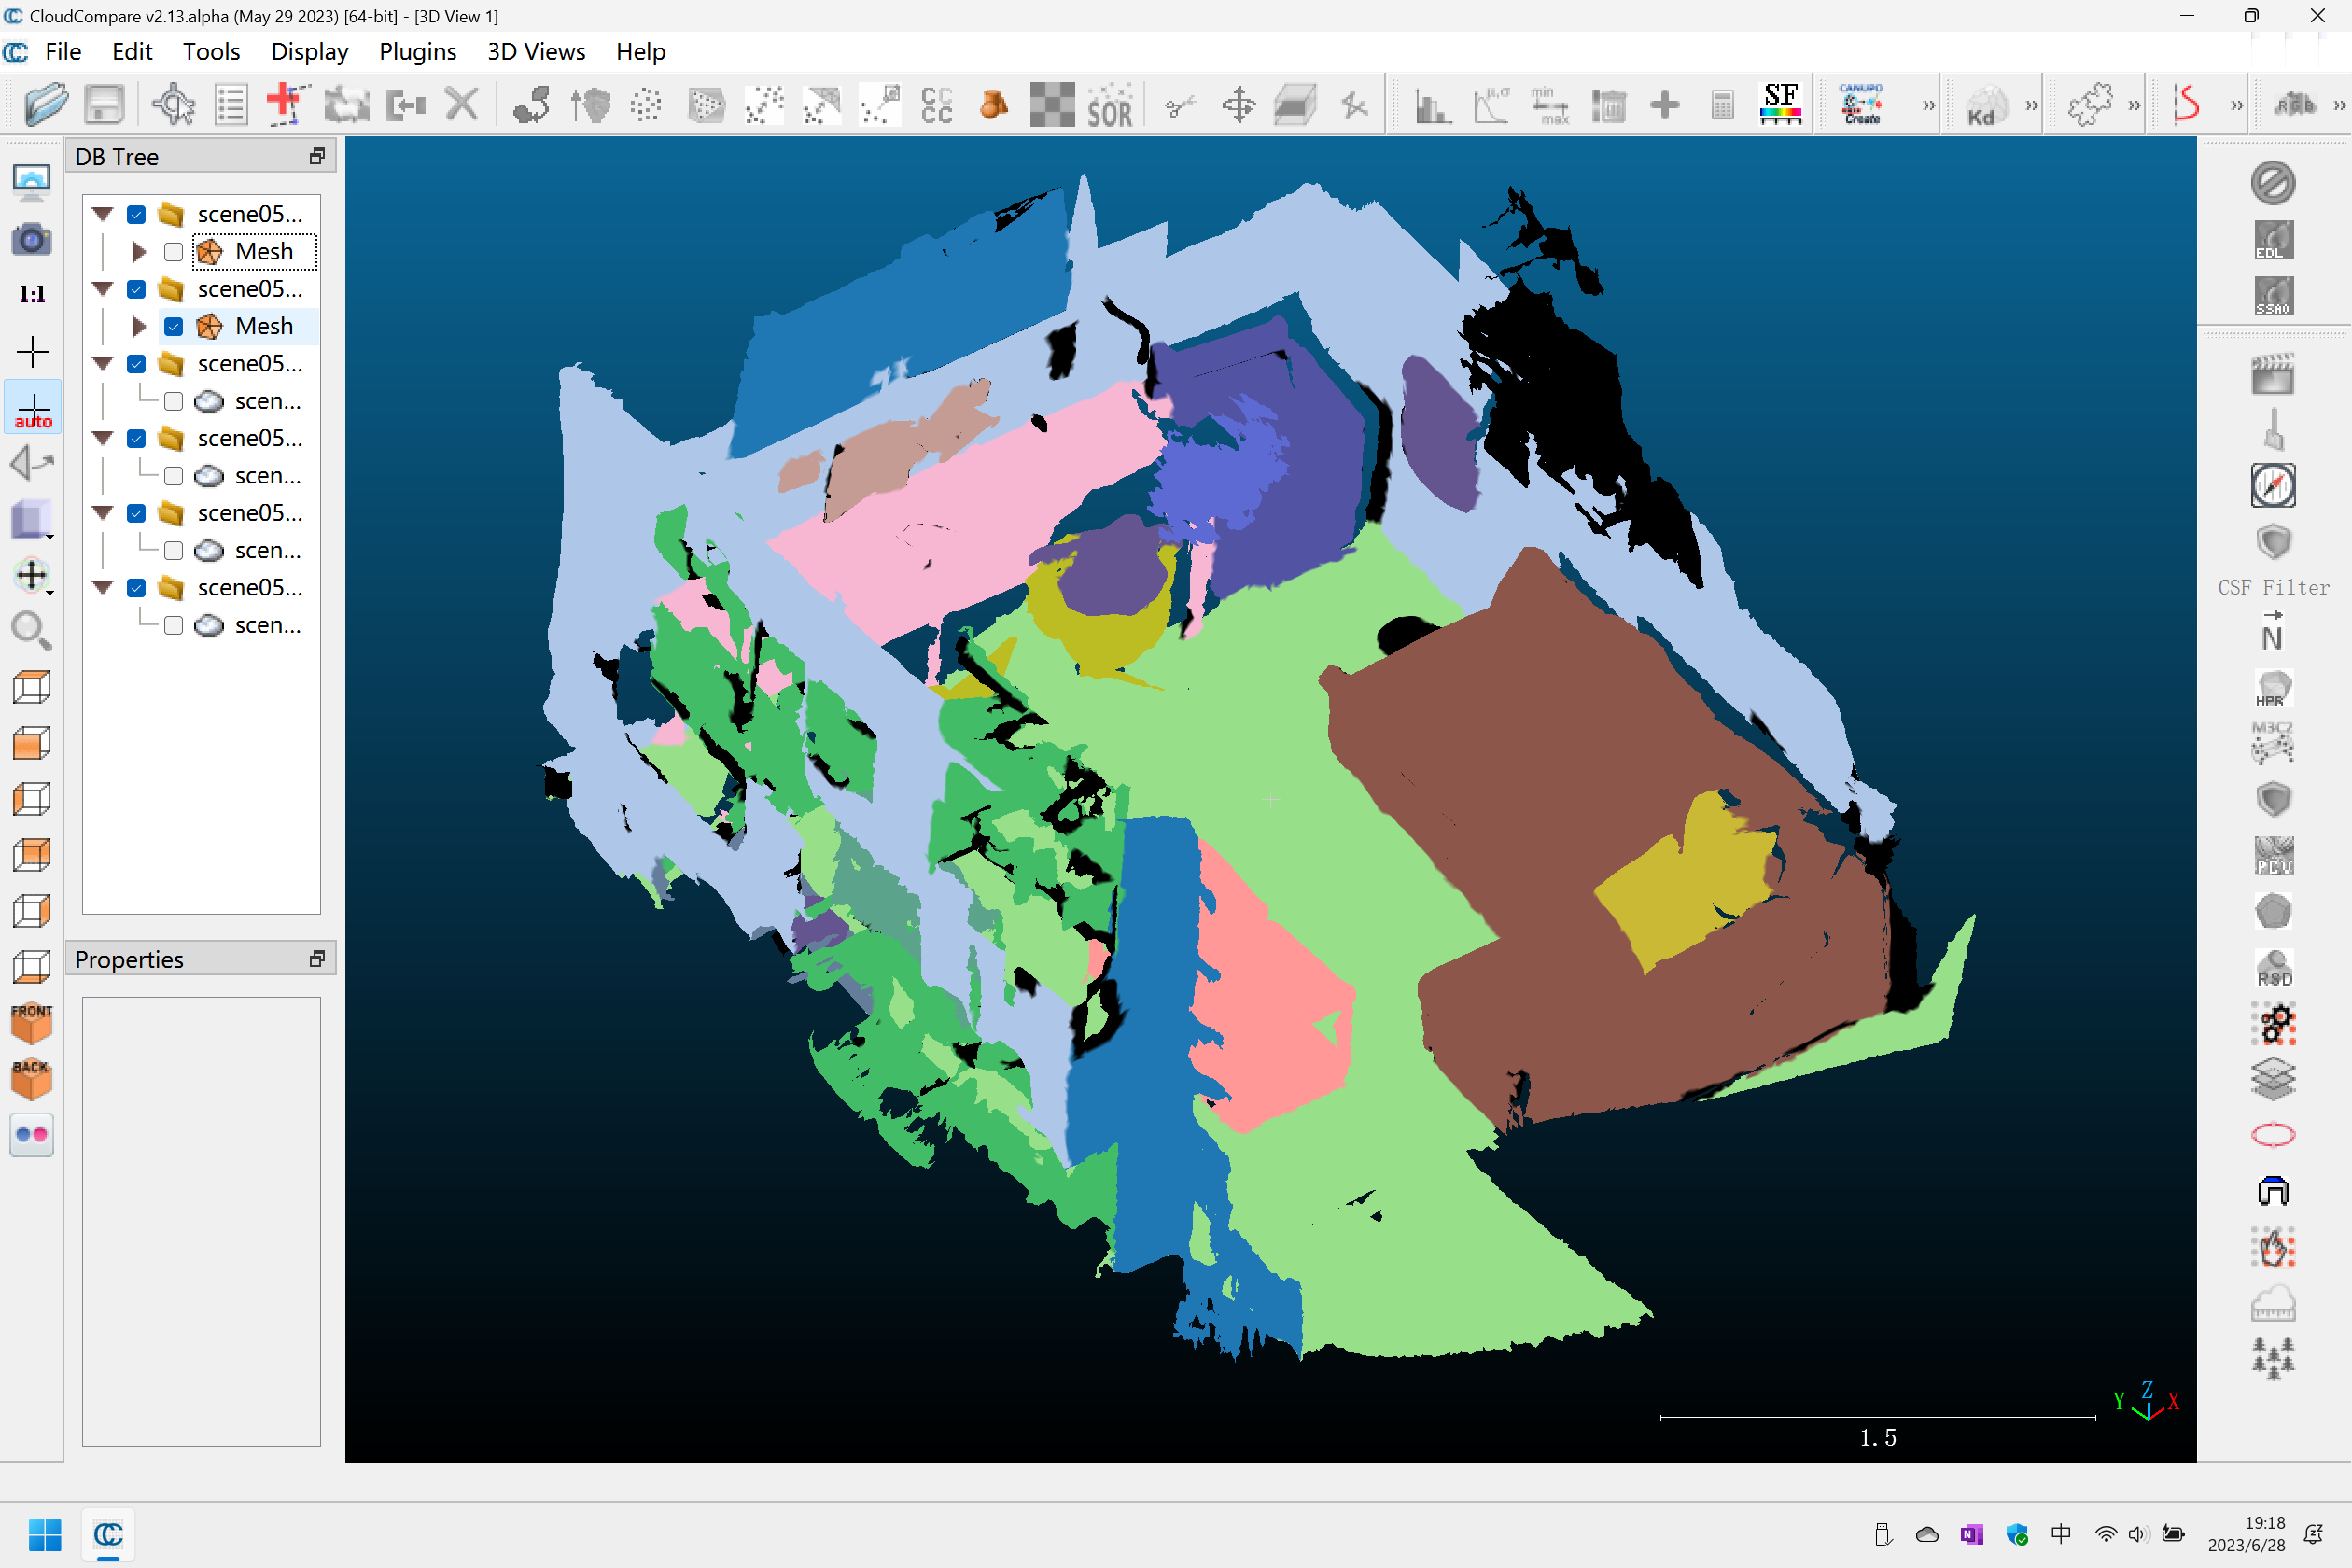
\includegraphics[width=1\textwidth]{figures/result/scene0518_label_gt.png}
		\end{minipage}
	}

	\subfigure[RGB信息2cm模型]{
		\begin{minipage}[t]{0.48\linewidth}
			\centering
			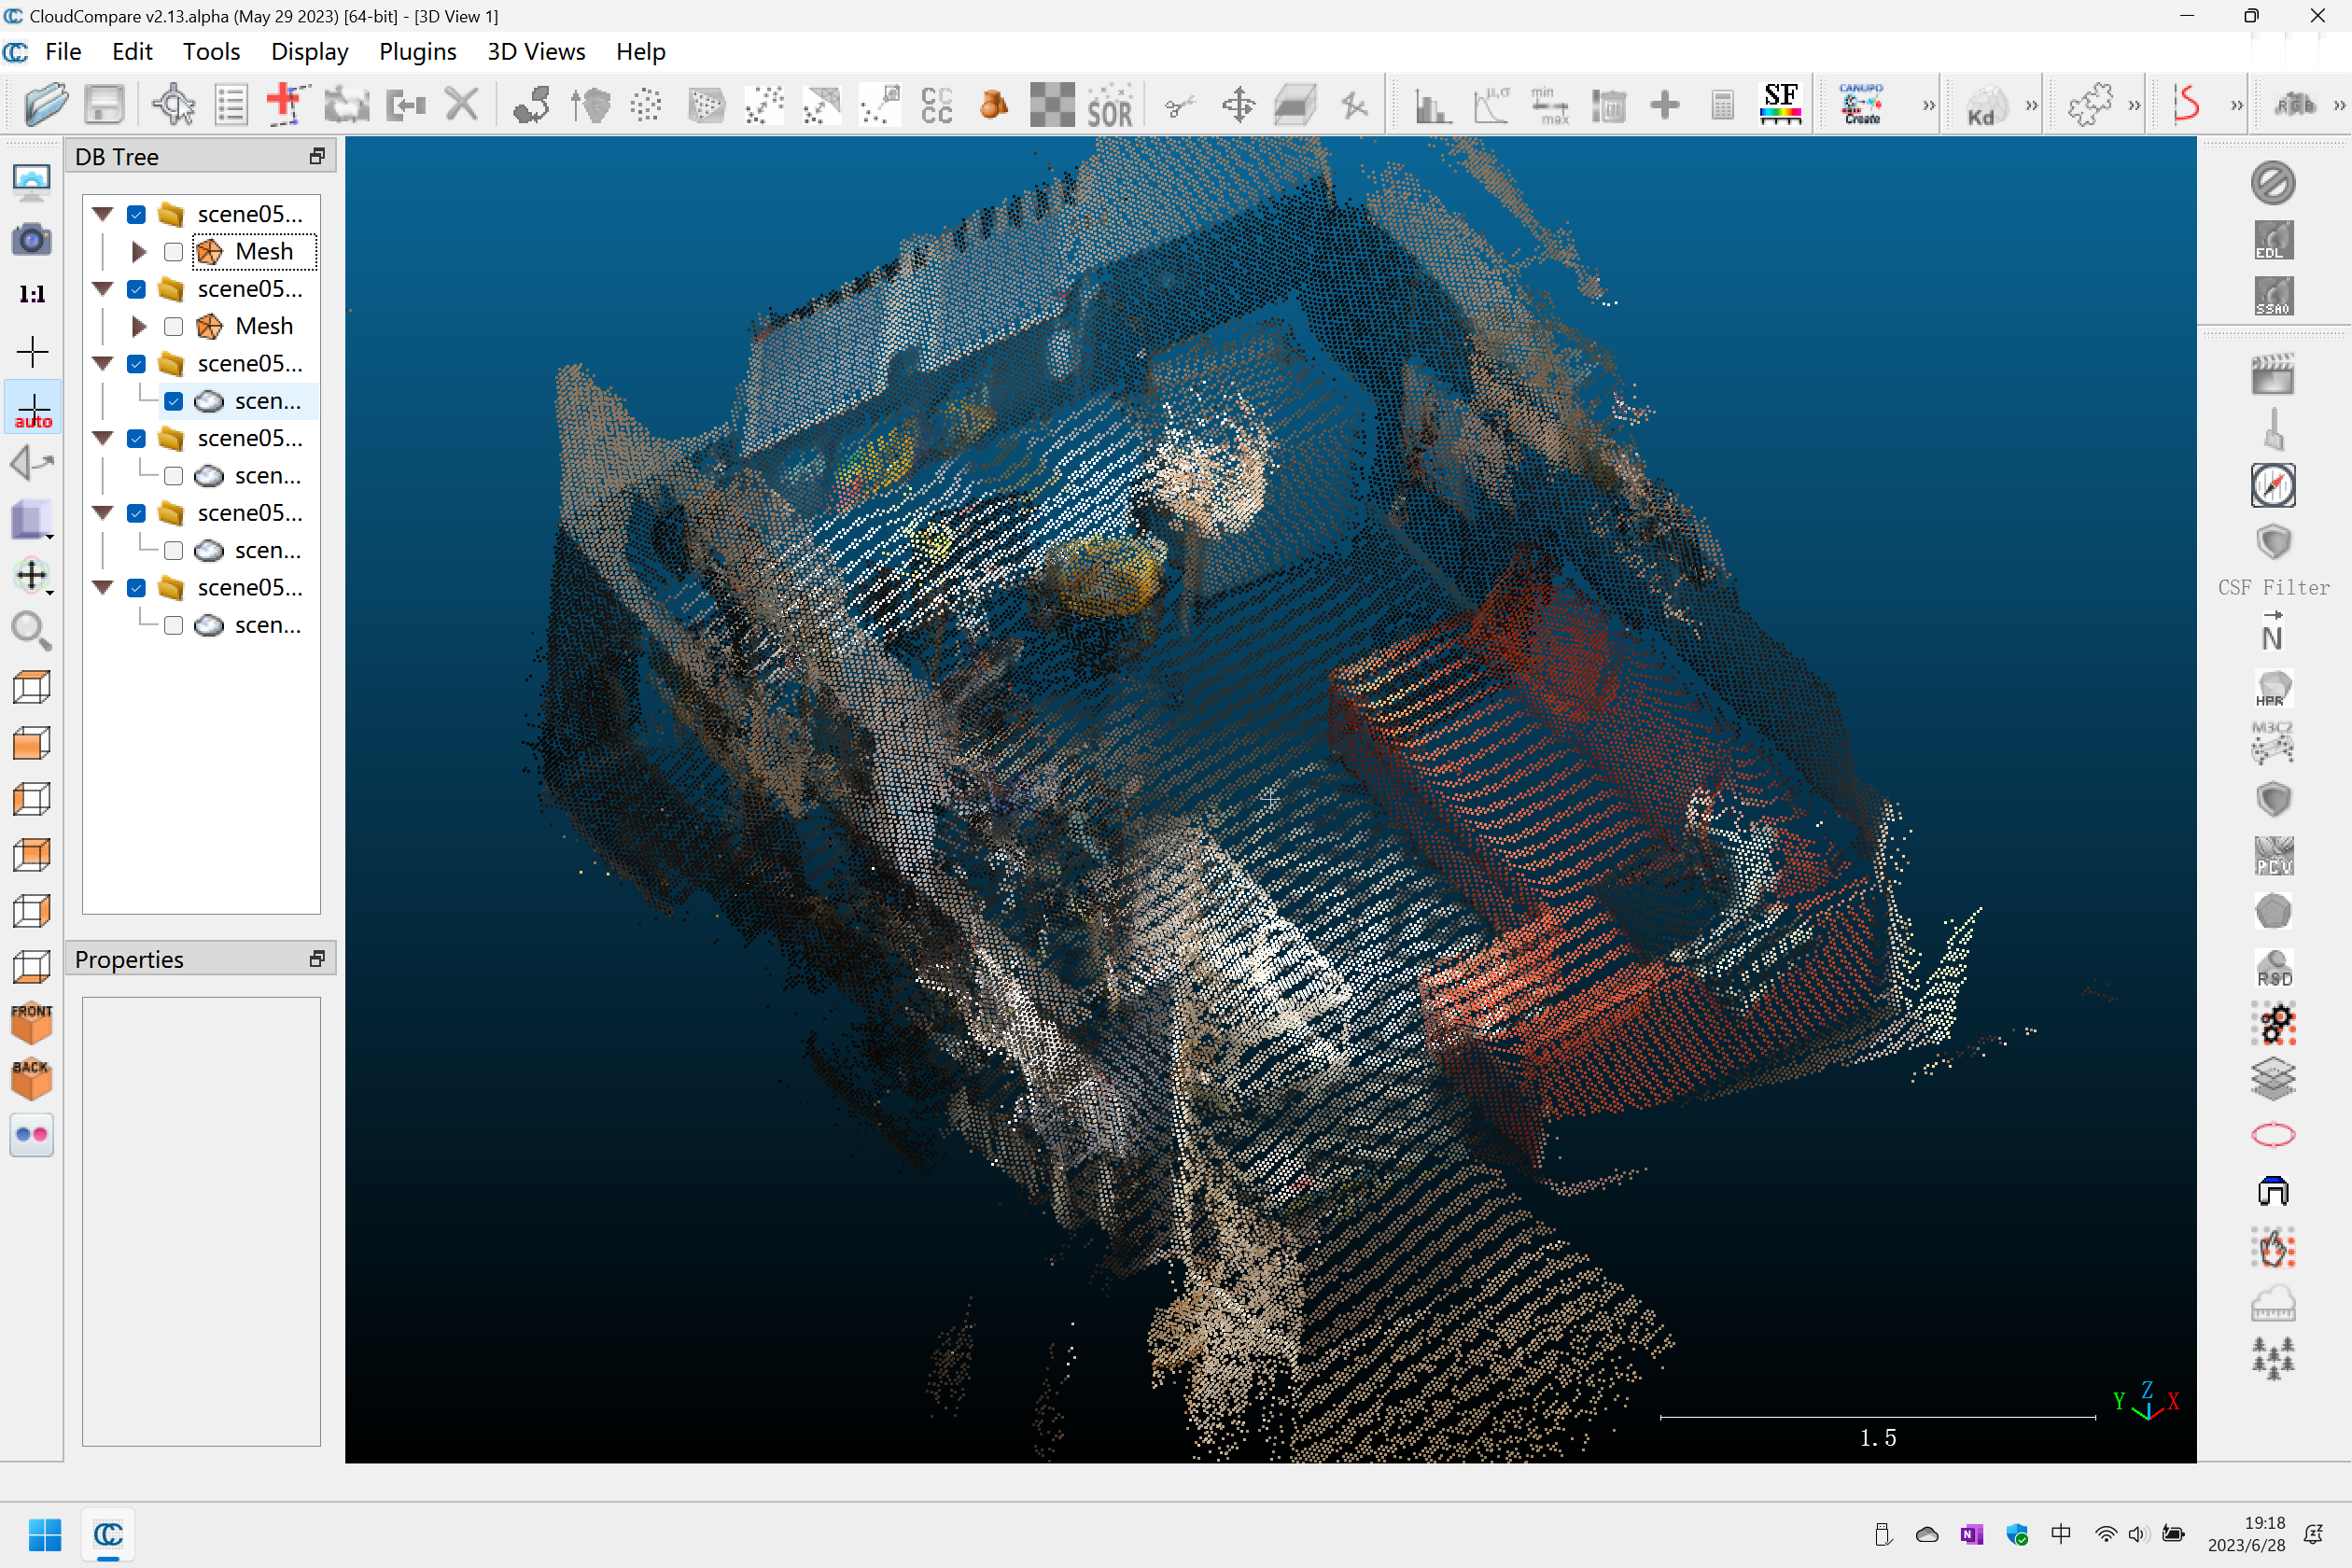
\includegraphics[width=1\textwidth]{figures/result/scene0518_rgb_2cm.png}
		\end{minipage}
	}
	\subfigure[语义信息2cm模型]{
		\begin{minipage}[t]{0.48\linewidth}
			\centering
			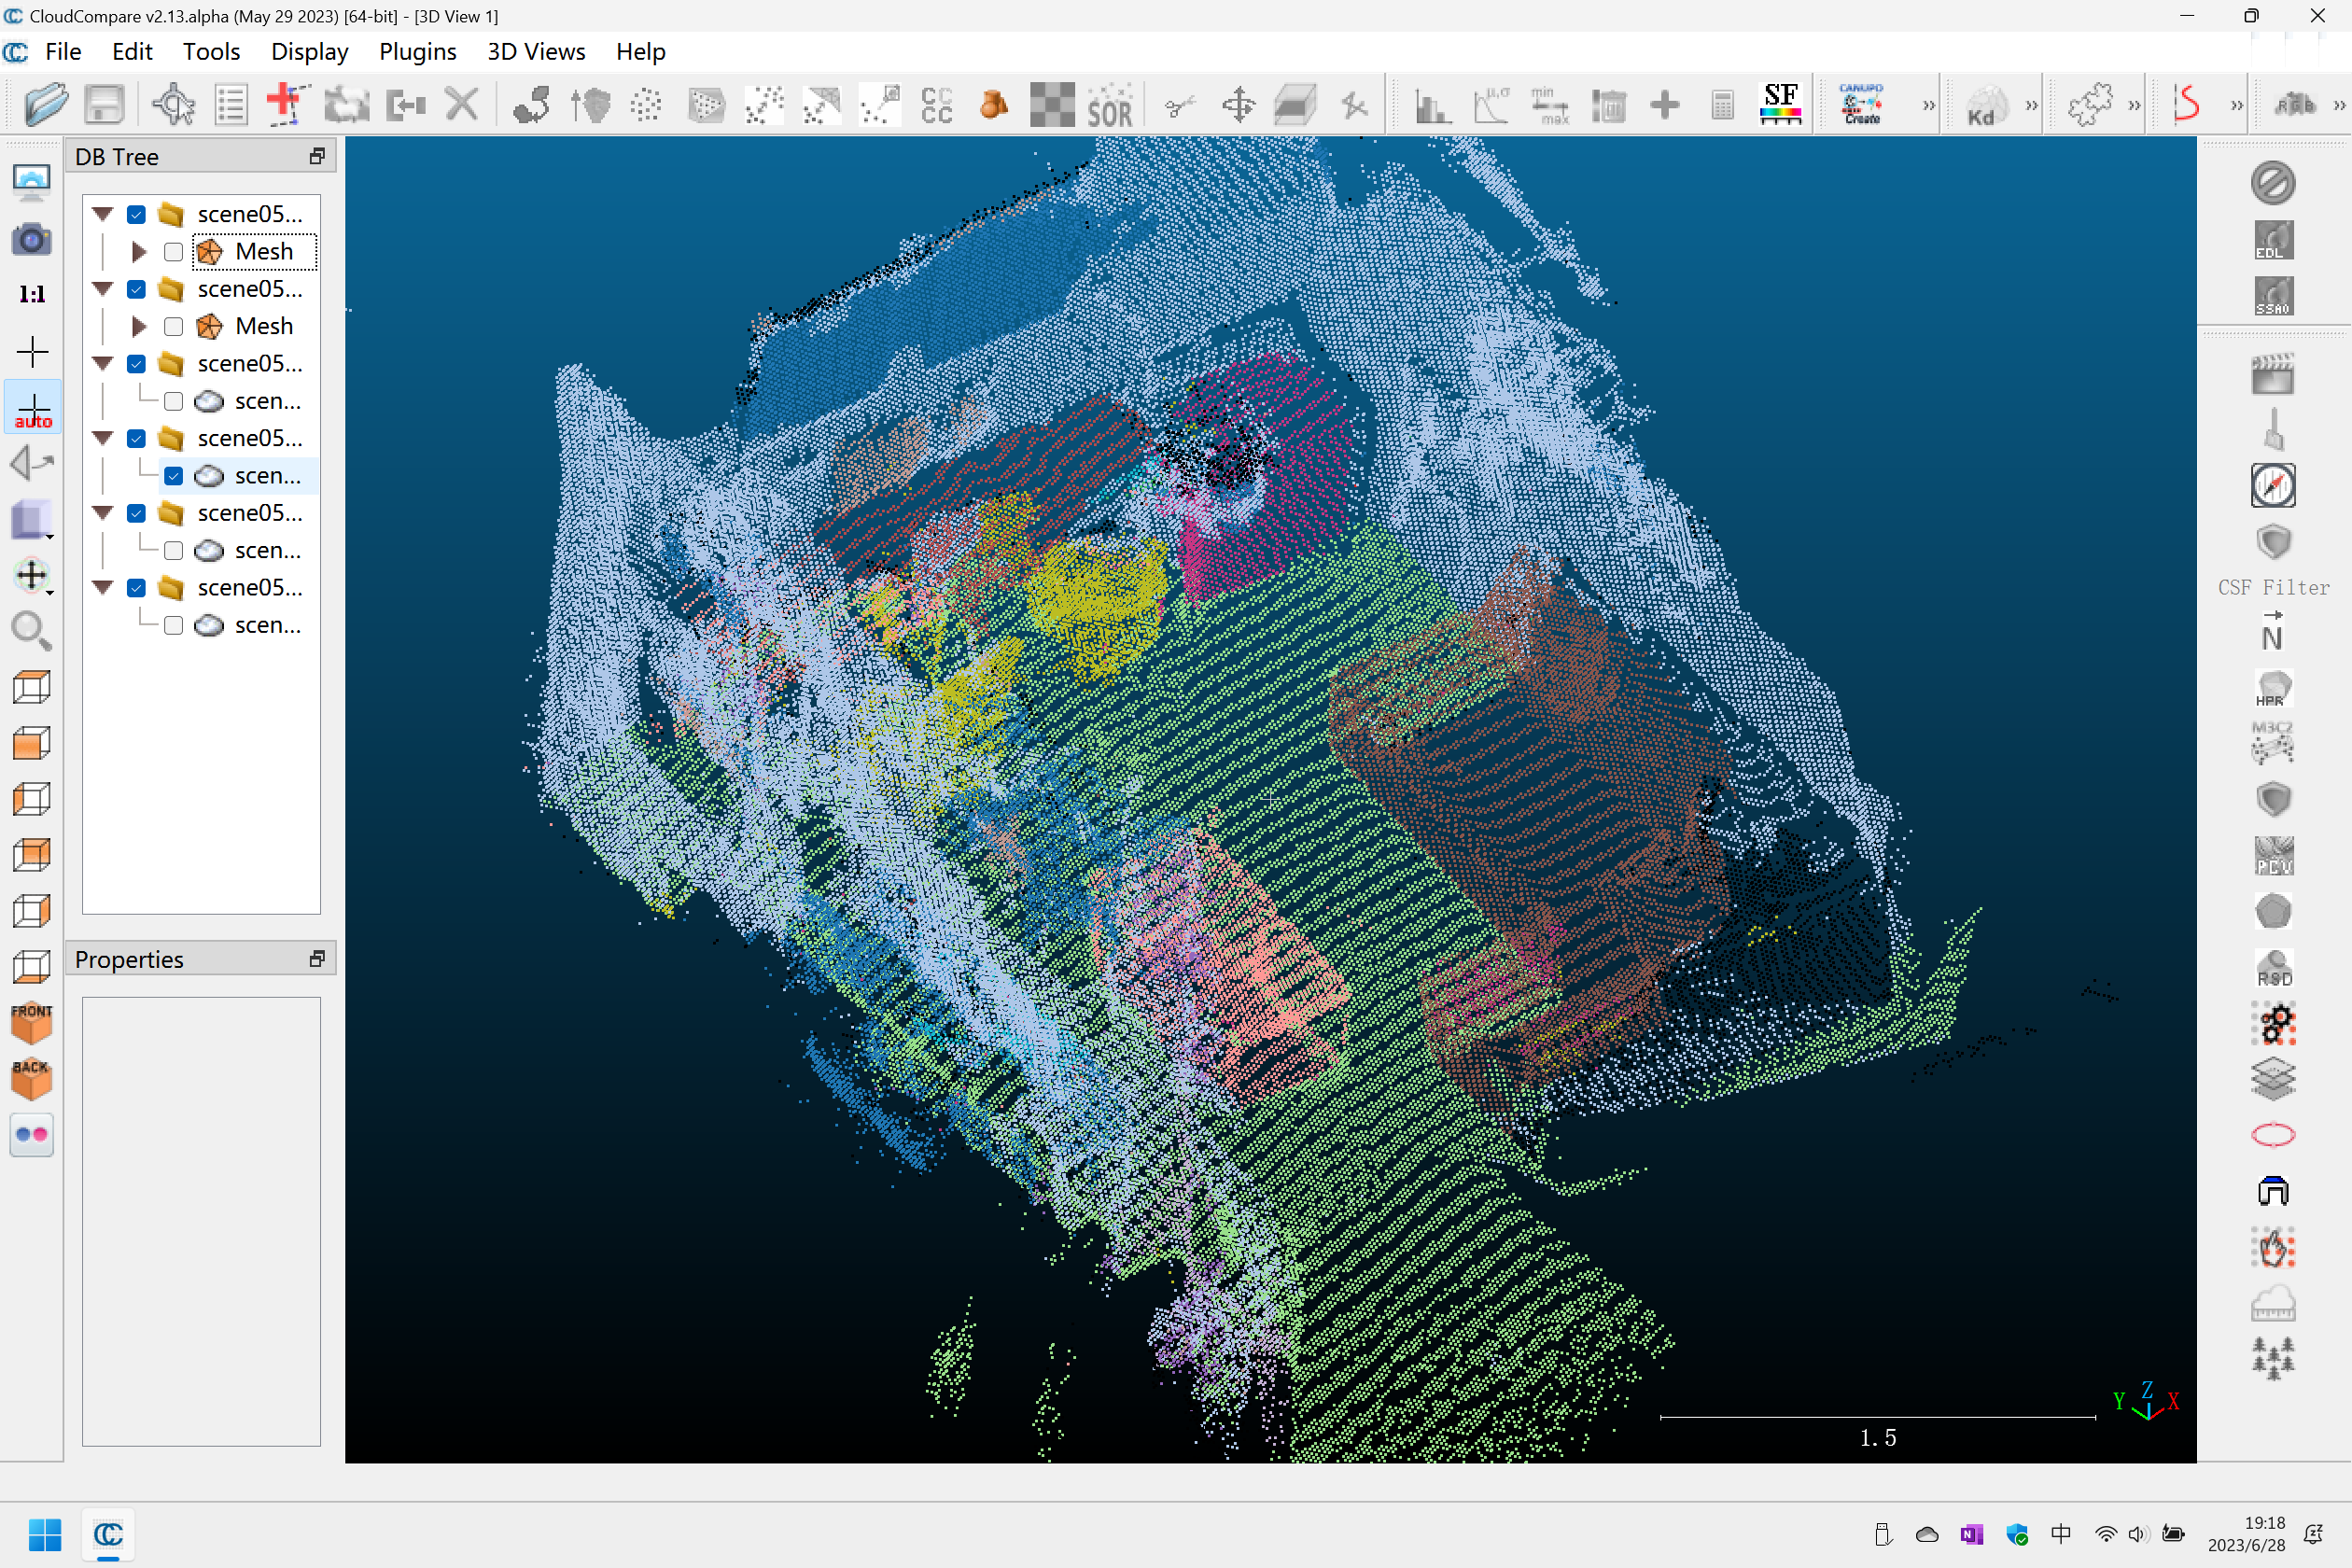
\includegraphics[width=1\textwidth]{figures/result/scene0518_label_2cm.png}
		\end{minipage}
	}

	\subfigure[RGB信息5cm模型]{
		\begin{minipage}[t]{0.48\linewidth}
			\centering
			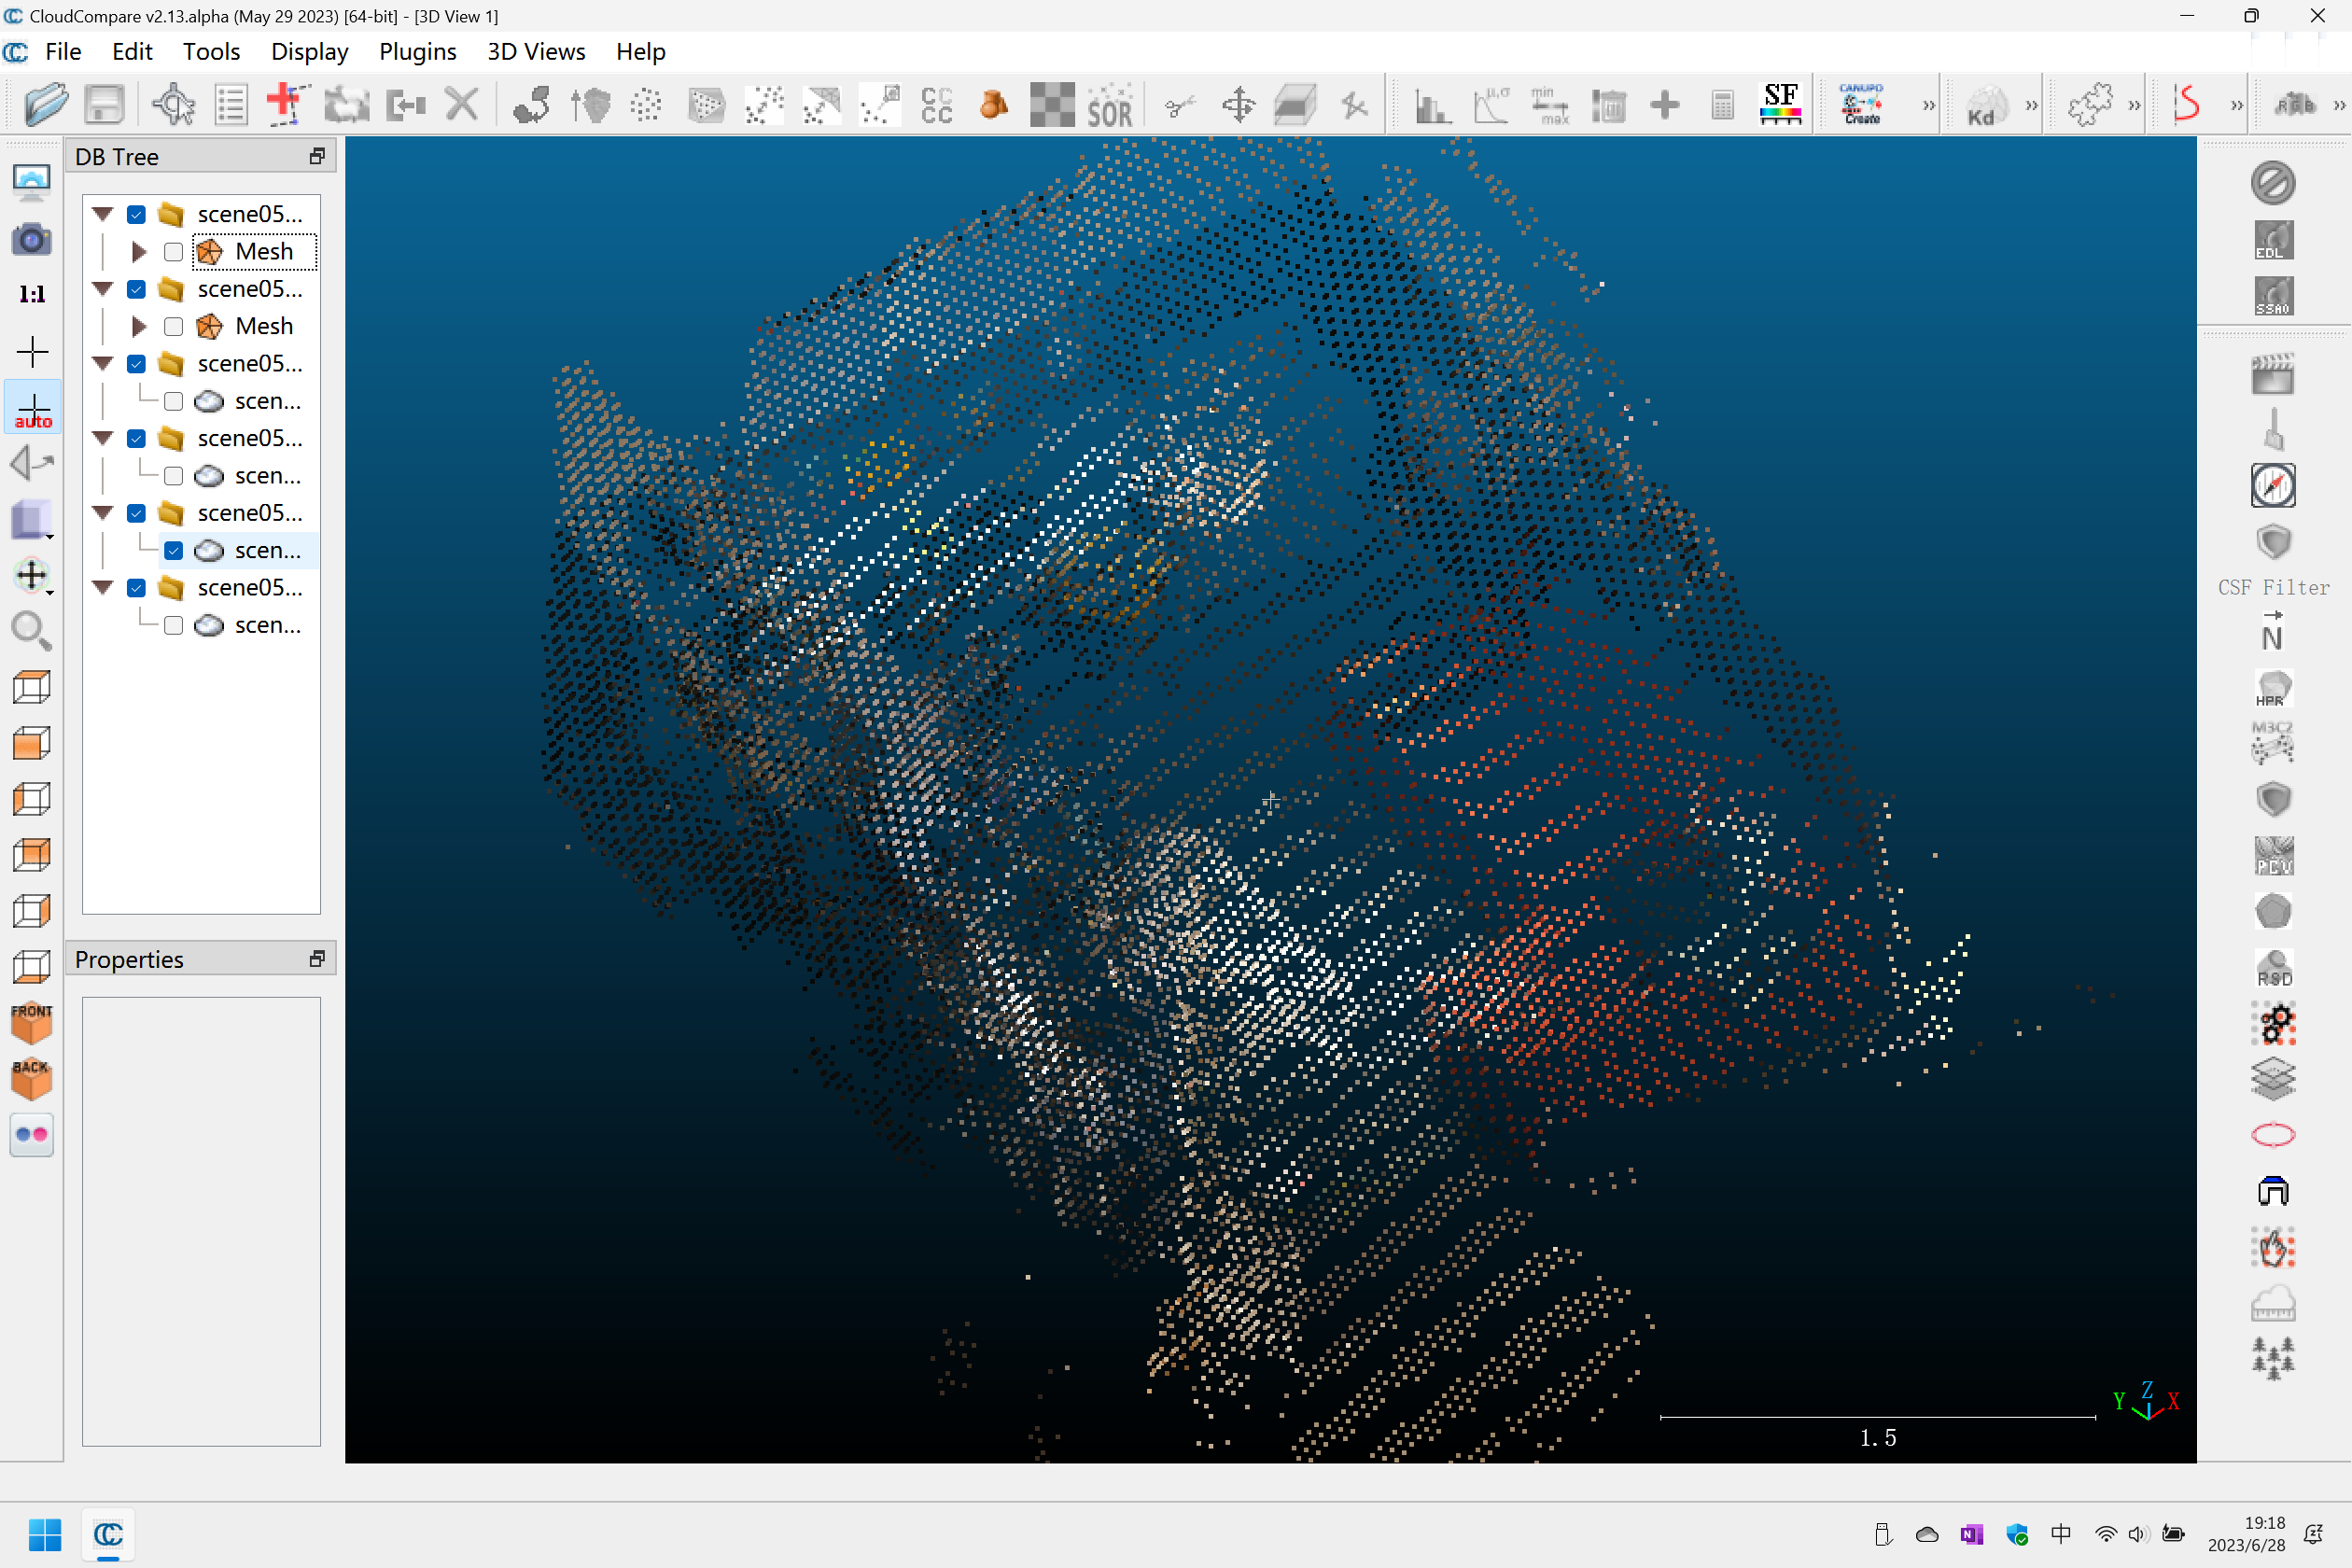
\includegraphics[width=1\textwidth]{figures/result/scene0518_rgb_5cm.png}
		\end{minipage}
	}
	\subfigure[语义信息5cm模型]{
		\begin{minipage}[t]{0.48\linewidth}
			\centering
			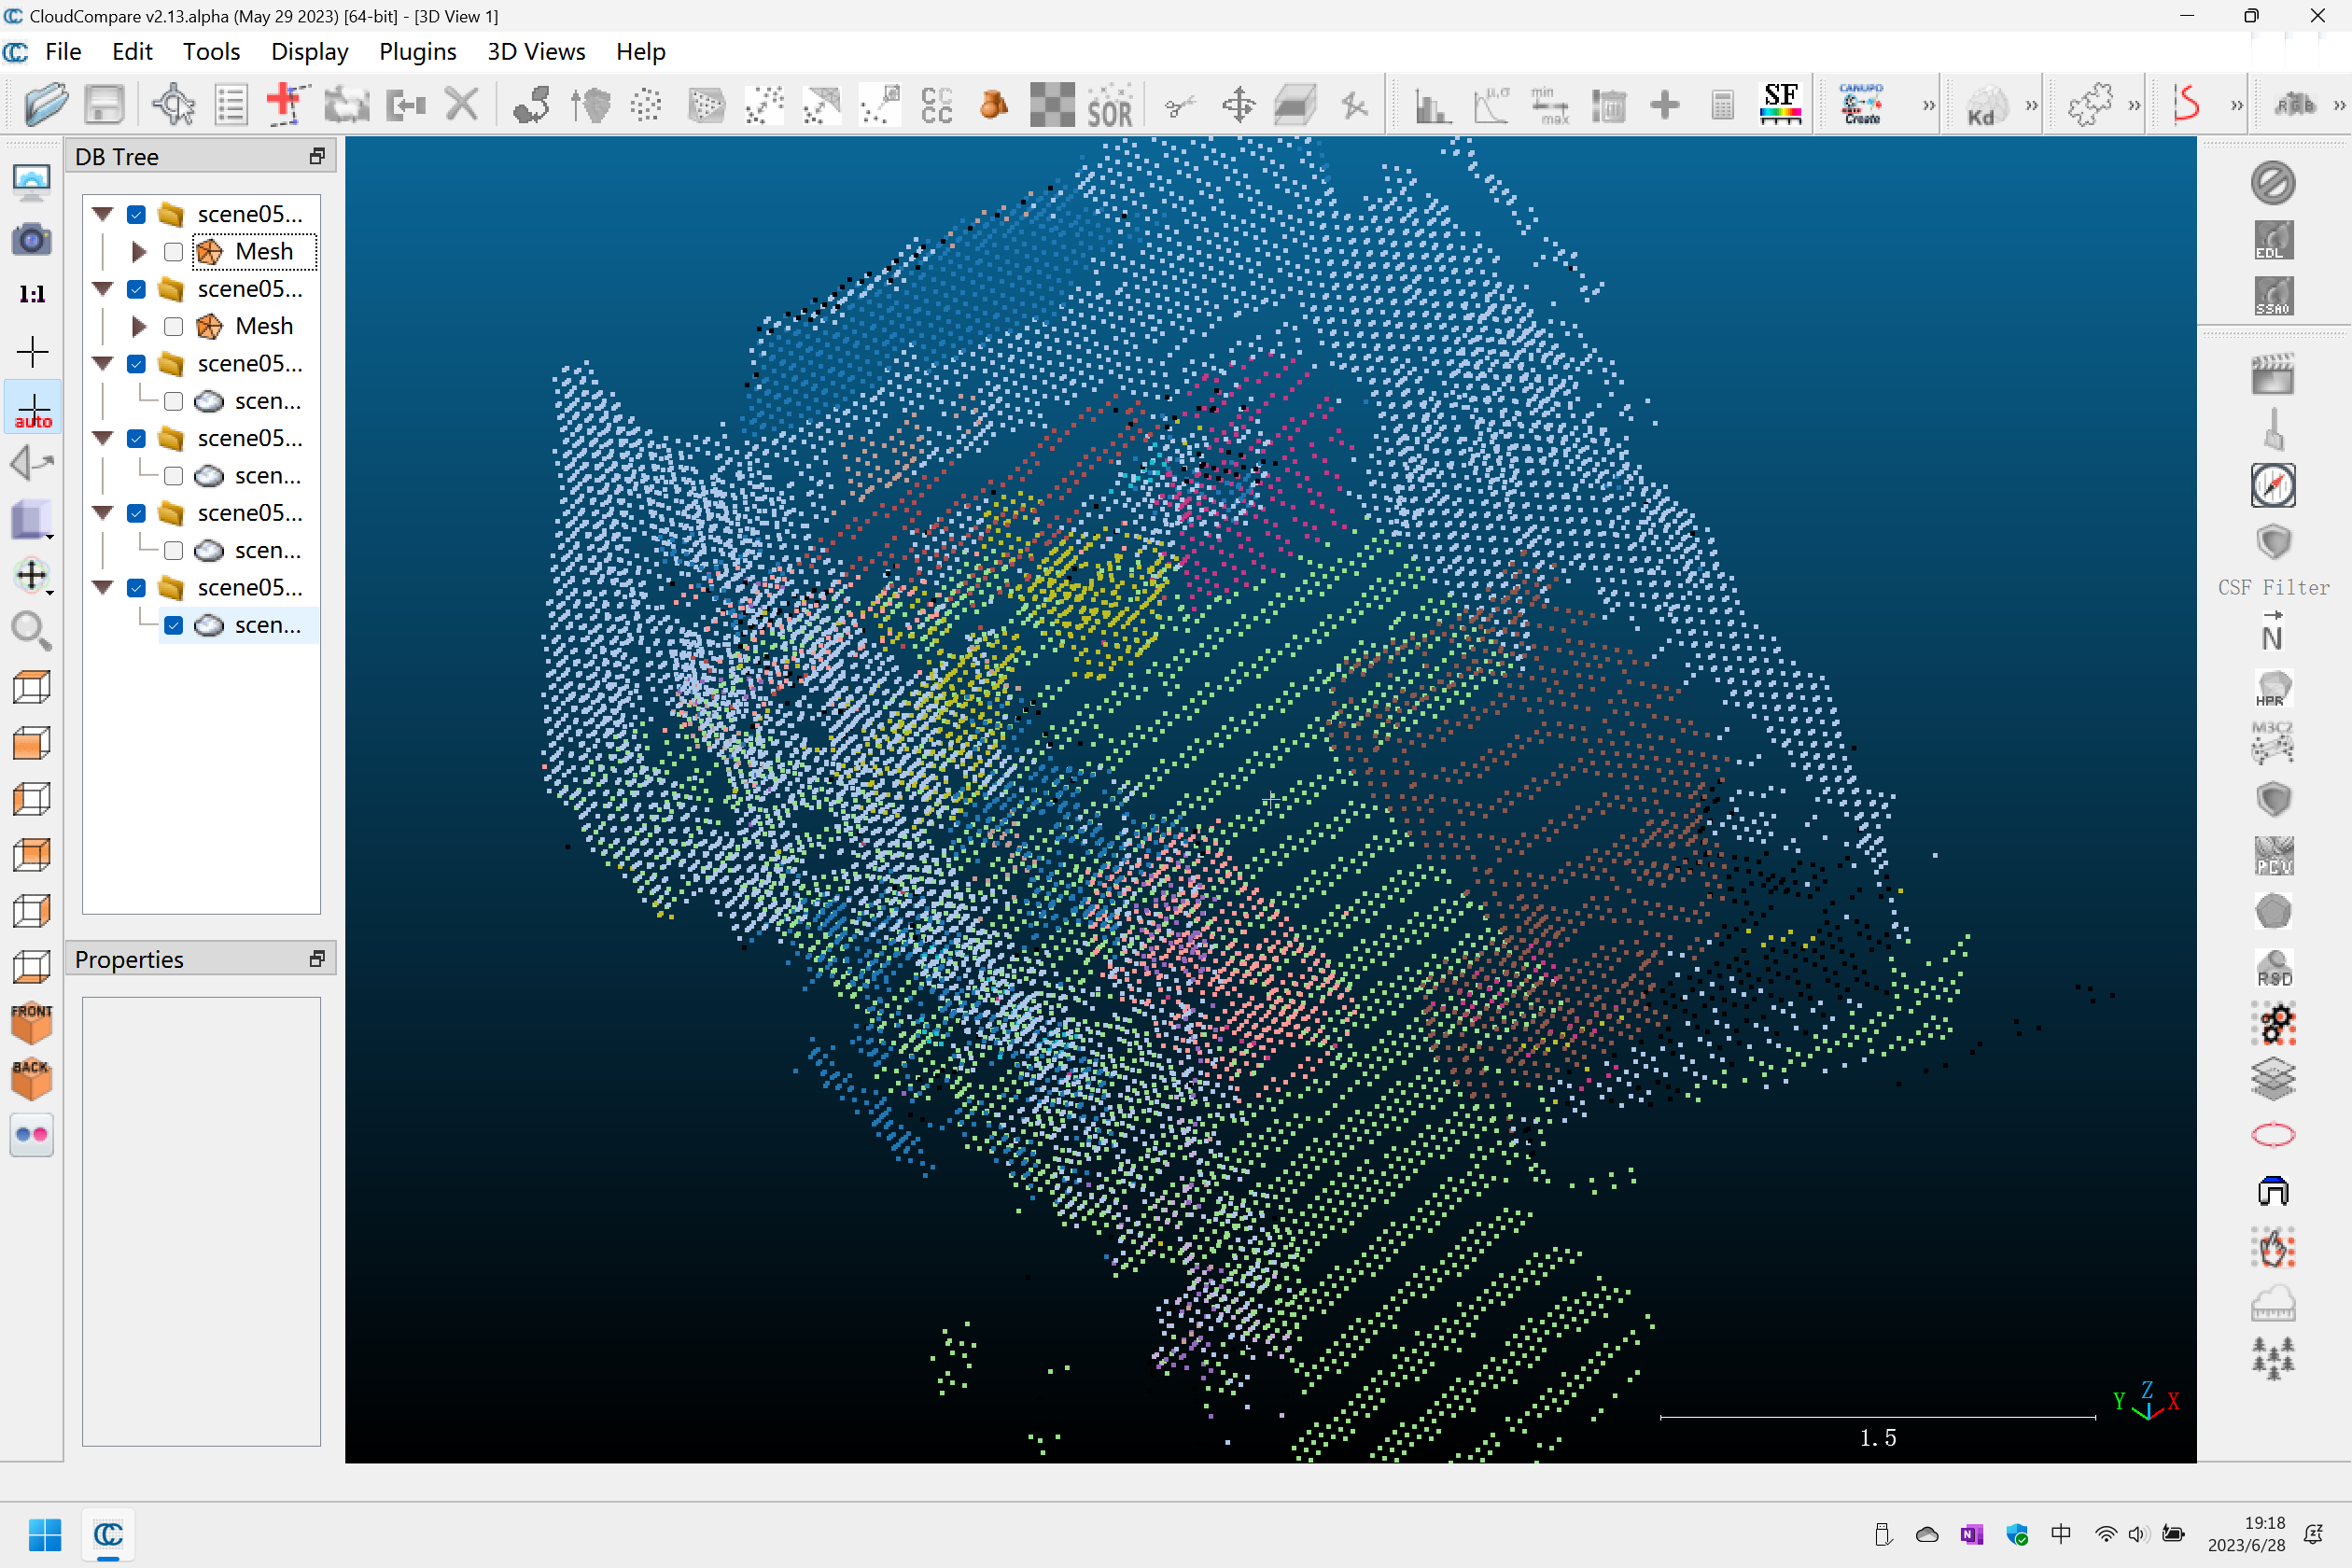
\includegraphics[width=1\textwidth]{figures/result/scene0518_label_5cm.png}
		\end{minipage}
	}
	\caption{场景scene0518\_00导出结果}
	\label{fig:scene0518_00_result}
\end{figure}